\documentclass{book}
\usepackage{graphicx}
\usepackage{hyperref}
\usepackage{amsmath}
\usepackage{amssymb}
\usepackage{amsfonts}
\usepackage{amsthm}
\usepackage{enumitem}
\usepackage{subcaption}
\usepackage{tikz}
\usetikzlibrary{arrows}
\usepackage{physics}
\usepackage{color}
\usepackage{dsfont}
\usepackage{array}

% environments
\definecolor{celadon}{rgb}{0.67, 0.88, 0.69}
\definecolor{teagreen}{rgb}{0.82, 0.94, 0.75}
% Math notations
\DeclareMathOperator*{\argmin}{arg\,min}
\DeclareMathOperator*{\argmax}{arg\,max}

\newcommand{\x}{\mathbf{x}}
\newcommand{\y}{\mathbf{y}}
\newcommand{\X}{\mathbf{X}}
\newcommand{\Y}{\mathbf{Y}}
\newcommand{\W}{\mathbf{W}} %Weight
\newcommand{\bias}{\mathbf{b}}%Bias
\newcommand{\act}{\texttt{g}}%Activation
\newcommand{\lr}{\eta} % learning rate
\newcommand{\loss}{L}
\newcommand{\pdata}{\hat{p}_{\texttt{data}}}
\newcommand{\nsize}{N}
\newcommand{\nfeatures}{P}
\newcommand{\param}{\boldsymbol{\theta}}
\newcommand{\featmap}{\boldsymbol{\phi}}
\newcommand{\EV}{\mathbb{E}}

\newcommand{\R}{\mathbb{R}}
\newcommand{\N}{\mathbb{N}}
\newcommand{\Z}{\mathbb{Z}}

\usepackage{physics}

\graphicspath{{../graphics/}}

\usepackage{tcolorbox}

\newtcolorbox{block}[1]{
    colback=white,
    colframe=black,
    fonttitle=\bfseries,
    title=#1,
    arc=2pt,
    boxrule=1pt
}

\newcommand{\alert}[1]{\textcolor{red}{#1}}


\title{Artificial Neural Networks and Backpropagation}
\author{E. Decencière}
\date{\today}

\begin{document}

\maketitle
\tableofcontents

\chapter{Artificial Neurons}

\section{Biological Neuron}

\begin{figure}[h]
    \centering
    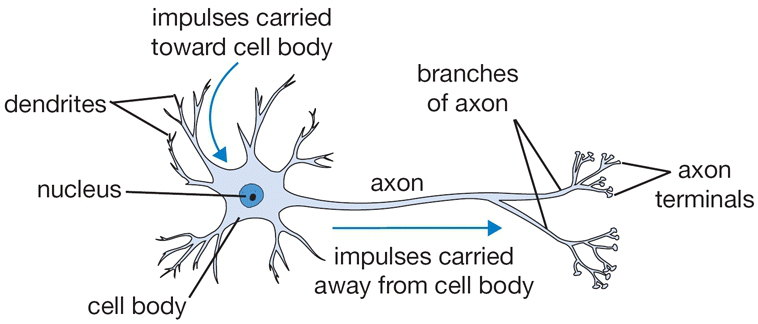
\includegraphics[height=3cm]{neuron}
\end{figure}

\begin{itemize}
\item A human neuron can have several thousand dendrites.
\item The neuron sends a signal through its axon if, during a given interval of time, the net input signal (sum of excitatory and inhibitory signals received through its dendrites) is larger than a threshold.
\end{itemize}

\section{Artificial Neuron}

\begin{figure}[h]
    \centering
    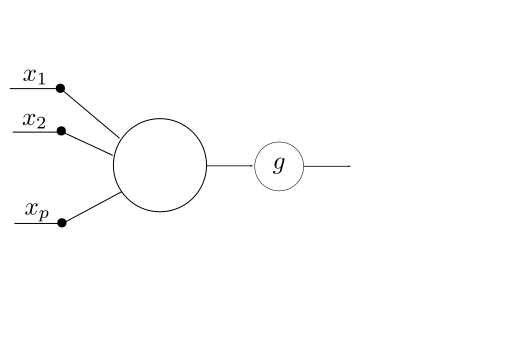
\includegraphics[height=3cm]{neurone_general}
\end{figure}

\begin{block}{General Principle}
An artificial neuron takes $p$ inputs $\{x_i\}_{1 \leq i \leq p}$, combines them to obtain a single value, and applies an activation function $\act$ to the result.
\end{block}

\begin{itemize}
\item The first artificial neuron model was proposed by \cite{mcculloch_logical_1943}.
\item Input and output signals were binary.
\item Input dendrites could be inhibitory or excitatory.
\end{itemize}

\section{Modern Artificial Neuron}

\begin{figure}[h]
    \centering
    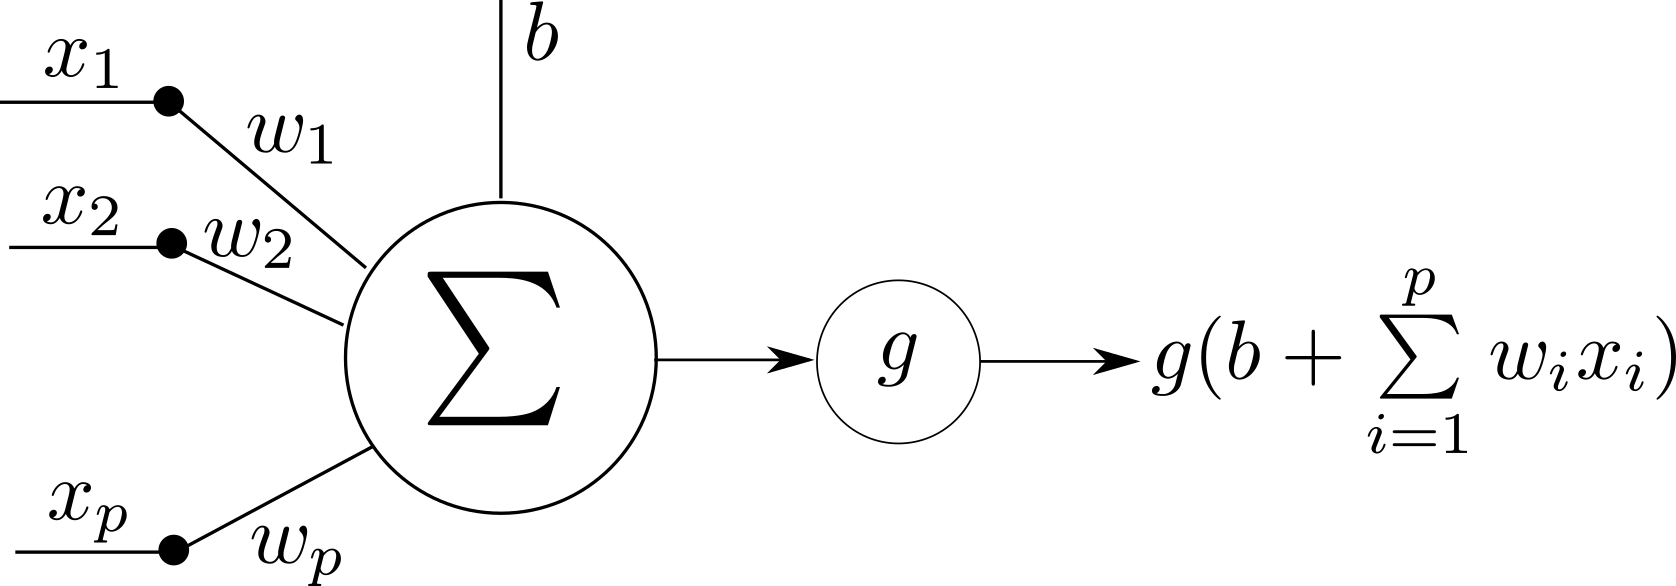
\includegraphics[height=3cm]{neurone}
\end{figure}

\begin{itemize}
\item The neuron computes a linear combination of the inputs $x_i$:
    \begin{itemize}
    \item The weights $w_i$ are multiplied with the inputs.
    \item The bias $b$ can be interpreted as a threshold on the sum.
    \end{itemize}
\item The activation function $\act$ decides, depending on its input, if a signal (the neuron's activation) is produced.
\end{itemize}

\section{The Role of the Activation Function}

\begin{figure}[h]
    \centering
    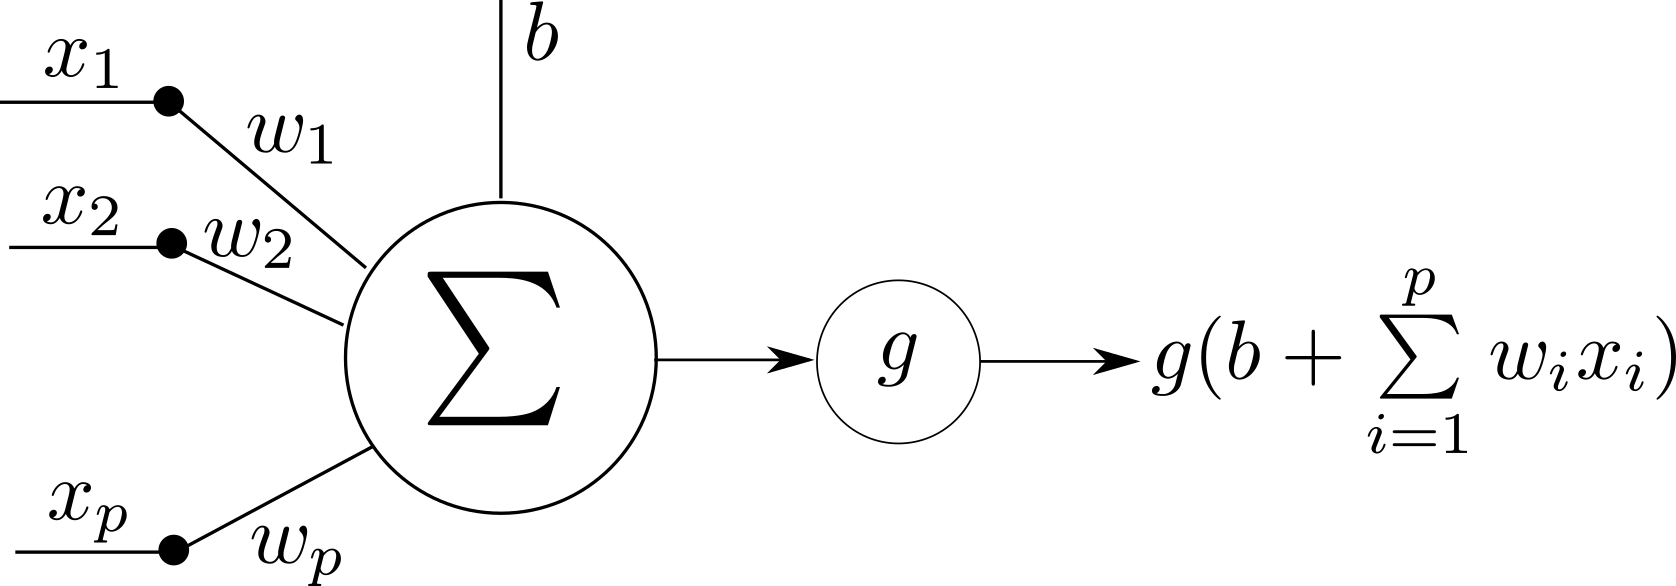
\includegraphics[height=3cm]{neurone}
\end{figure}

\begin{itemize}
\item The initial idea behind the activation function is that it works as a gate.
\item If its input is ``high enough'', then the neuron is activated, i.e., a signal (other than zero) is produced.
\item It can be interpreted as a source of abstraction: information considered as unimportant is ignored (or reduced).
\end{itemize}

\section{Activation Functions}

\subsection{Binary Activation}

\begin{figure}[h]
    \centering
    \begin{subfigure}{.5\textwidth}
        \[
        \act(x)=
        \begin{cases}
        1, & \text{if } x > 0\\
        0, & \text{otherwise}
        \end{cases}
        \]
    \end{subfigure}
    \begin{subfigure}{.5\textwidth}
        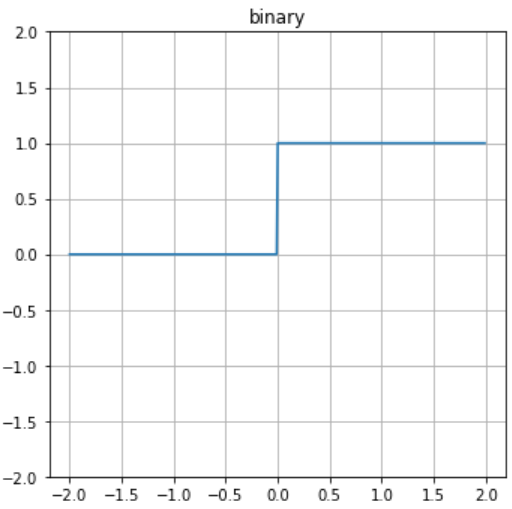
\includegraphics[width=.8\textwidth]{act_bin.png}
    \end{subfigure}
\end{figure}

\begin{block}{Remarks}
\begin{itemize}
\item Biologically inspired.
\item[+] Simple to compute.
\item[+] High abstraction.
\item[-] Gradient nil except on one point.
\item \alert{In practice, almost never used.}
\end{itemize}
\end{block}

\subsection{Sigmoid Activation}

\begin{figure}[h]
    \centering
    \begin{subfigure}{.5\textwidth}
        \[
        \act(x)= \frac{1}{1 + e^{-x}} = \frac{e^{x}}{1+e^{x}}
        \]
    \end{subfigure}
    \begin{subfigure}{.5\textwidth}
        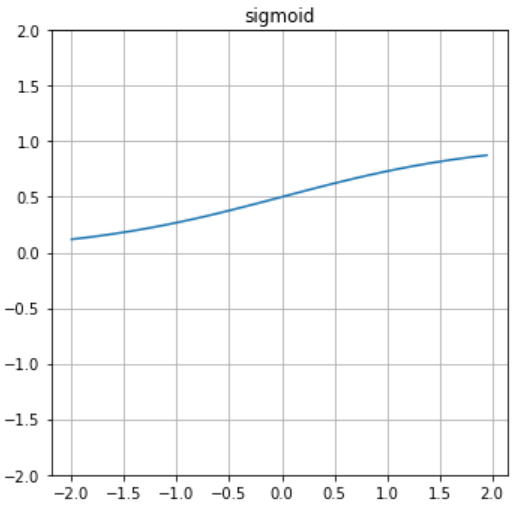
\includegraphics[width=.8\textwidth]{act_sigm.png}
    \end{subfigure}
\end{figure}

\begin{block}{Remarks}
\begin{itemize}
\item[+] Similar to binary activation, but with usable gradient.
\item Bijection between $\R$ and $]0, 1[$: no loss of information.
\item[-] Gradient tends to zero as we get away from zero.
\item[-] More computationally intensive.
\end{itemize}
\end{block}

\subsection{Hyperbolic Tangent Activation}

\begin{figure}[h]
    \centering
    \begin{subfigure}{.5\textwidth}
        \[
        \act(x)= \frac{e^x - e^{-x}}{e^x + e^{-x}}
        \]
    \end{subfigure}
    \begin{subfigure}{.5\textwidth}
        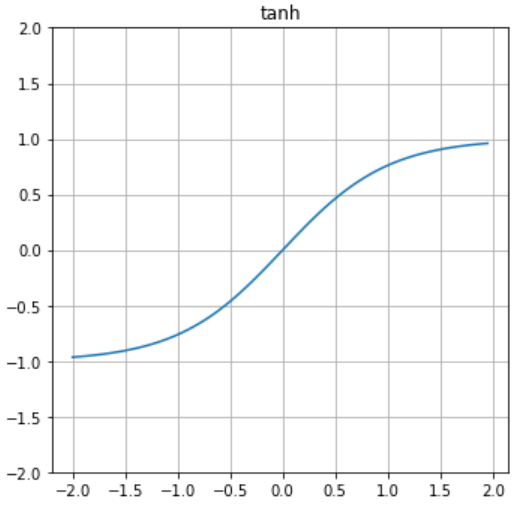
\includegraphics[width=.8\textwidth]{act_tanh.png}
    \end{subfigure}
\end{figure}

\begin{block}{Remarks}
\begin{itemize}
\item Similar to sigmoid.
\end{itemize}
\end{block}

\subsection{Rectified Linear Unit (ReLU) Activation}

\begin{figure}[h]
    \centering
    \begin{subfigure}{.5\textwidth}
        \[
        \act(x)=
        \begin{cases}
        x, & \text{if } x > 0\\
        0, & \text{otherwise}
        \end{cases}
        \]
    \end{subfigure}
    \begin{subfigure}{.5\textwidth}
        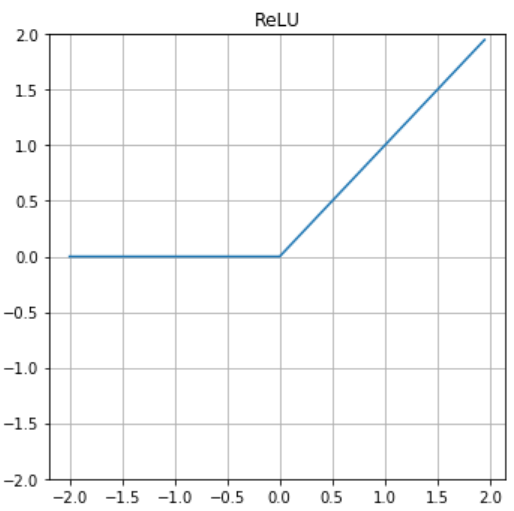
\includegraphics[width=.8\textwidth]{act_relu.png}
    \end{subfigure}
\end{figure}

\begin{block}{Remarks}
\begin{itemize}
\item[+] Usable gradient when activated.
\item[+] Fast to compute.
\item[+] High abstraction.
\end{itemize}
\end{block}

\section{What Can an Artificial Neuron Compute?}

\begin{figure}[h]
    \centering
    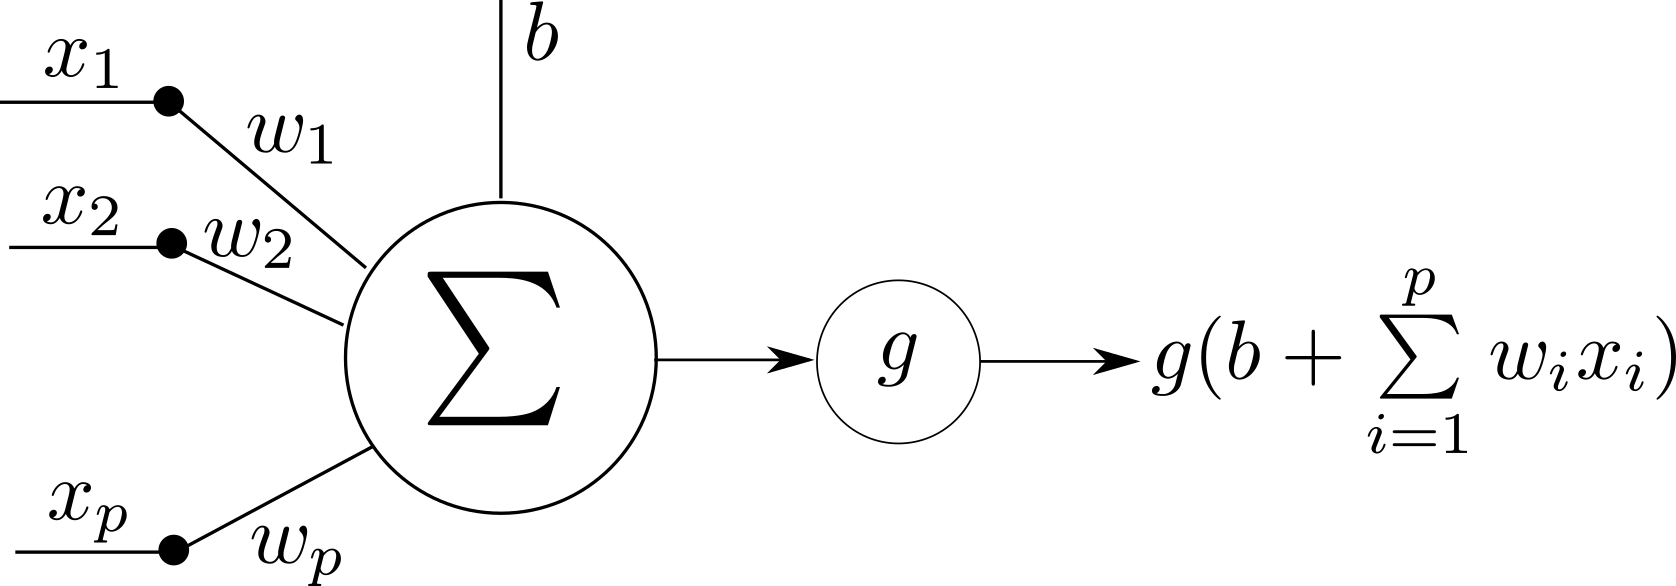
\includegraphics[height=3cm]{neurone}
\end{figure}

\begin{block}{}
In $\R^p$, $b + \sum\limits_{i=1}^p w_ix_i = 0$ corresponds to a hyperplane $H$. For a given point $\x = \{x_1, \ldots, x_p\}$, decisions are made according to the side of the hyperplane it belongs to.
\end{block}

\section{Example in 2D}

\begin{figure}[h]
    \centering
    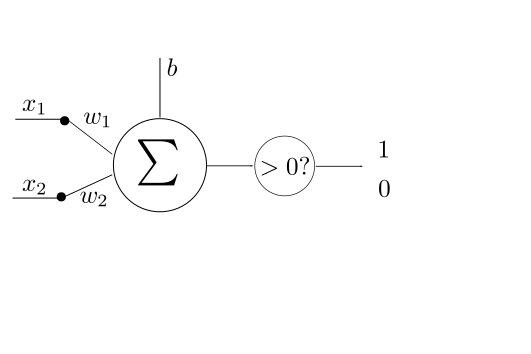
\includegraphics[height=3cm]{neurone_simple}
\end{figure}

\begin{itemize}
\item $p=2$: 2-dimensional inputs (can be represented on a screen!).
\item Activation: binary.
\item Classification problem.
\end{itemize}

\section{Gaussian Clouds}

\begin{figure}[h]
    \centering
    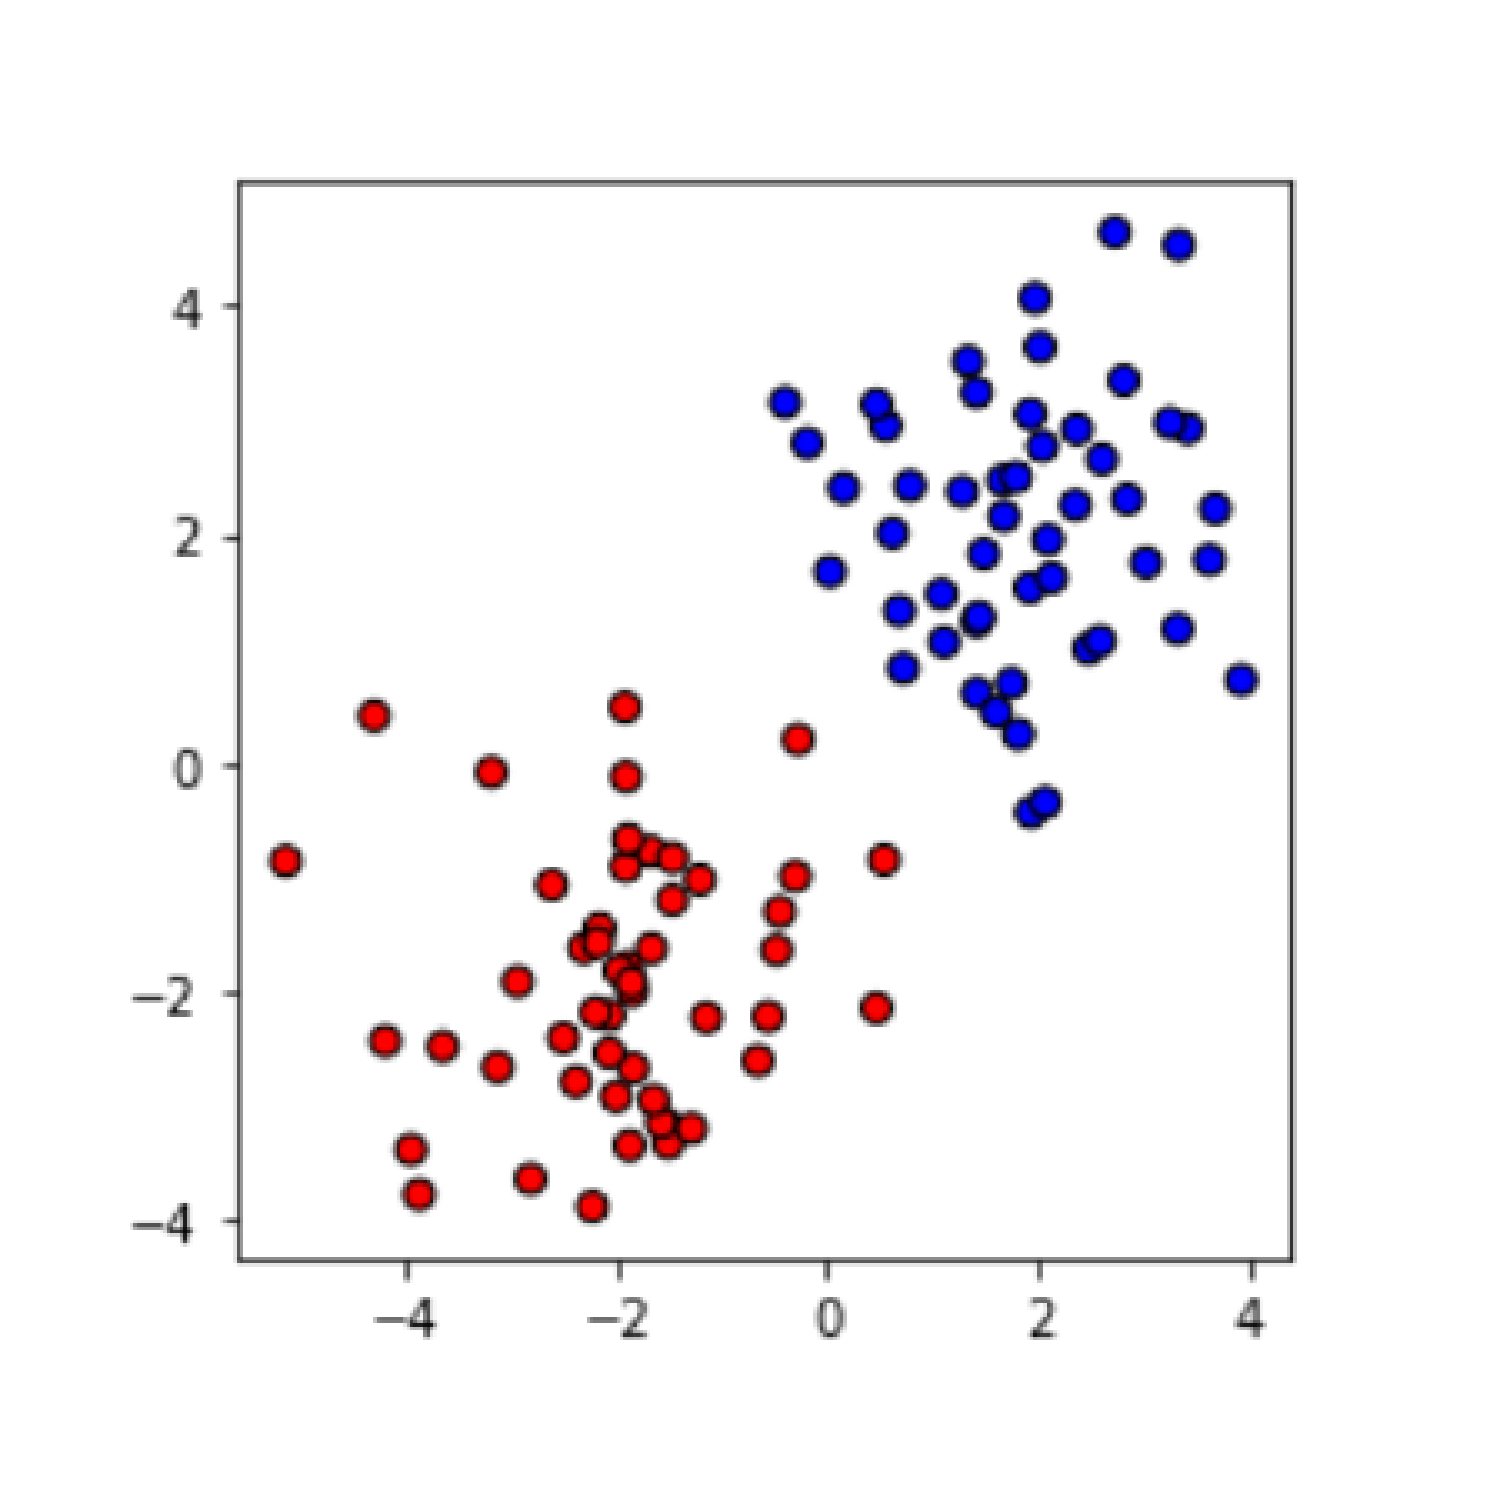
\includegraphics[height=6cm]{gaussian_clouds}
\end{figure}

\section{Circles}

\begin{figure}[h]
    \centering
    \includegraphics[height=6cm]{circles}
\end{figure}

\section{Solution with a Simple Neural Network}

\begin{figure}[h]
    \centering
    \begin{subfigure}{.5\textwidth}
        \includegraphics[height=5cm]{ann_5}
    \end{subfigure}
    \begin{subfigure}{.5\textwidth}
        \includegraphics[height=4cm]{circles_H}
    \end{subfigure}
\end{figure}

\begin{block}{Intuition}
Combining several neurons, one can build complex classifiers.
\end{block}

\section{Compact Representation}

\begin{figure}[h]
    \centering
    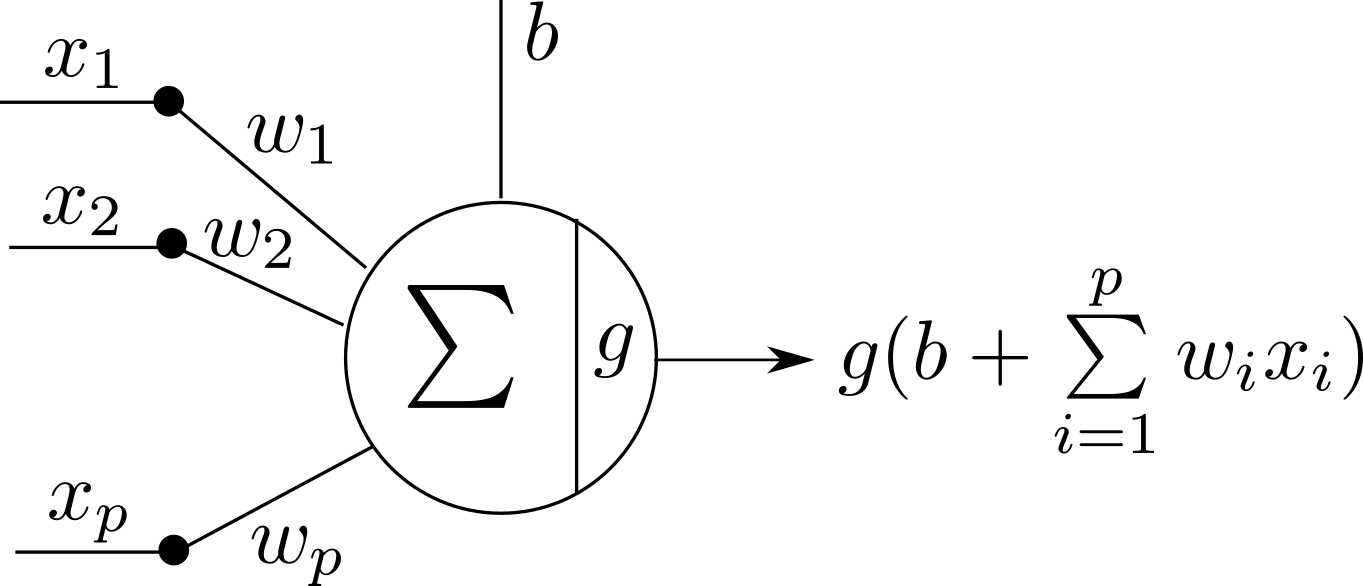
\includegraphics[height=3cm]{neurone_representation_compacte}
\end{figure}

\section{Notations}

\begin{figure}[h]
    \centering
    \begin{subfigure}{.5\textwidth}
        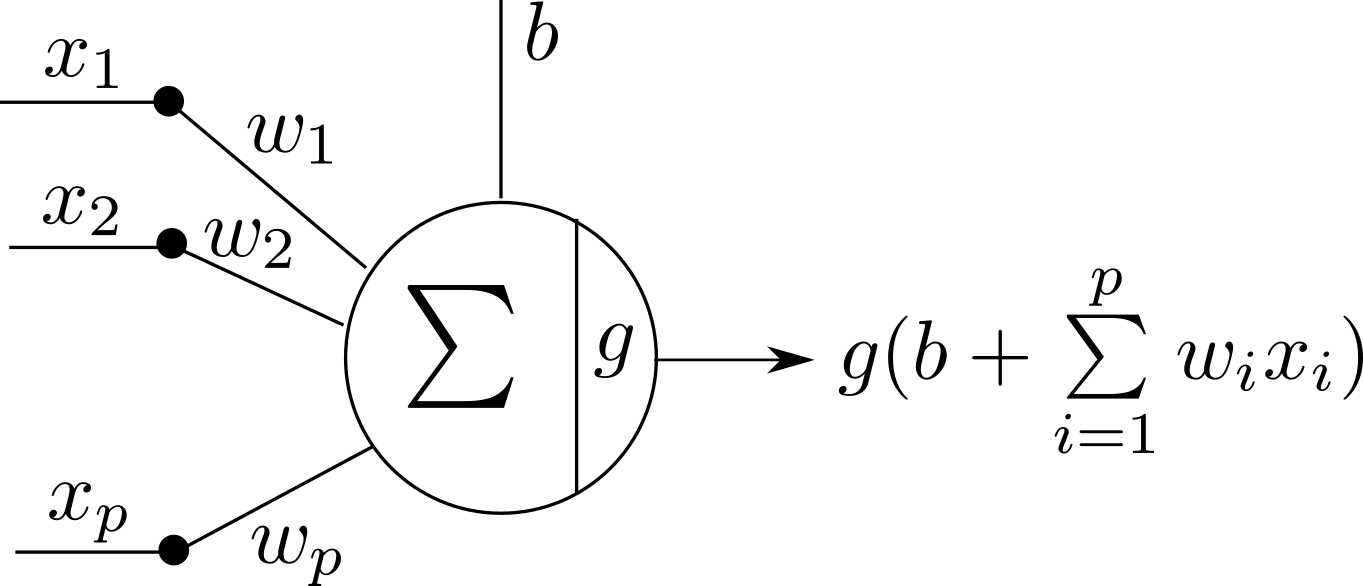
\includegraphics[height=2cm]{neurone_representation_compacte}
    \end{subfigure}
    \begin{subfigure}{.5\textwidth}
        With
        \[
        \mathbf{w} =
        \begin{pmatrix}
        w_1 \\
        \vdots \\
        w_p
        \end{pmatrix}
        = (w_1, \ldots, w_p)^T
        \]
        and
        \[
        \x =
        \begin{pmatrix}
        x_1 \\
        \vdots \\
        x_p
        \end{pmatrix}
        = (x_1, \ldots, x_p)^T
        \]
    \end{subfigure}
\end{figure}

We can simply write:
\[
\act(b+ \sum\limits_{i=1}^p w_ix_i) = \act(b + \mathbf{w}^T\x)
\]

\chapter{Artificial Neural Networks}

\section{Computational Graph}

\begin{figure}[h]
    \centering
    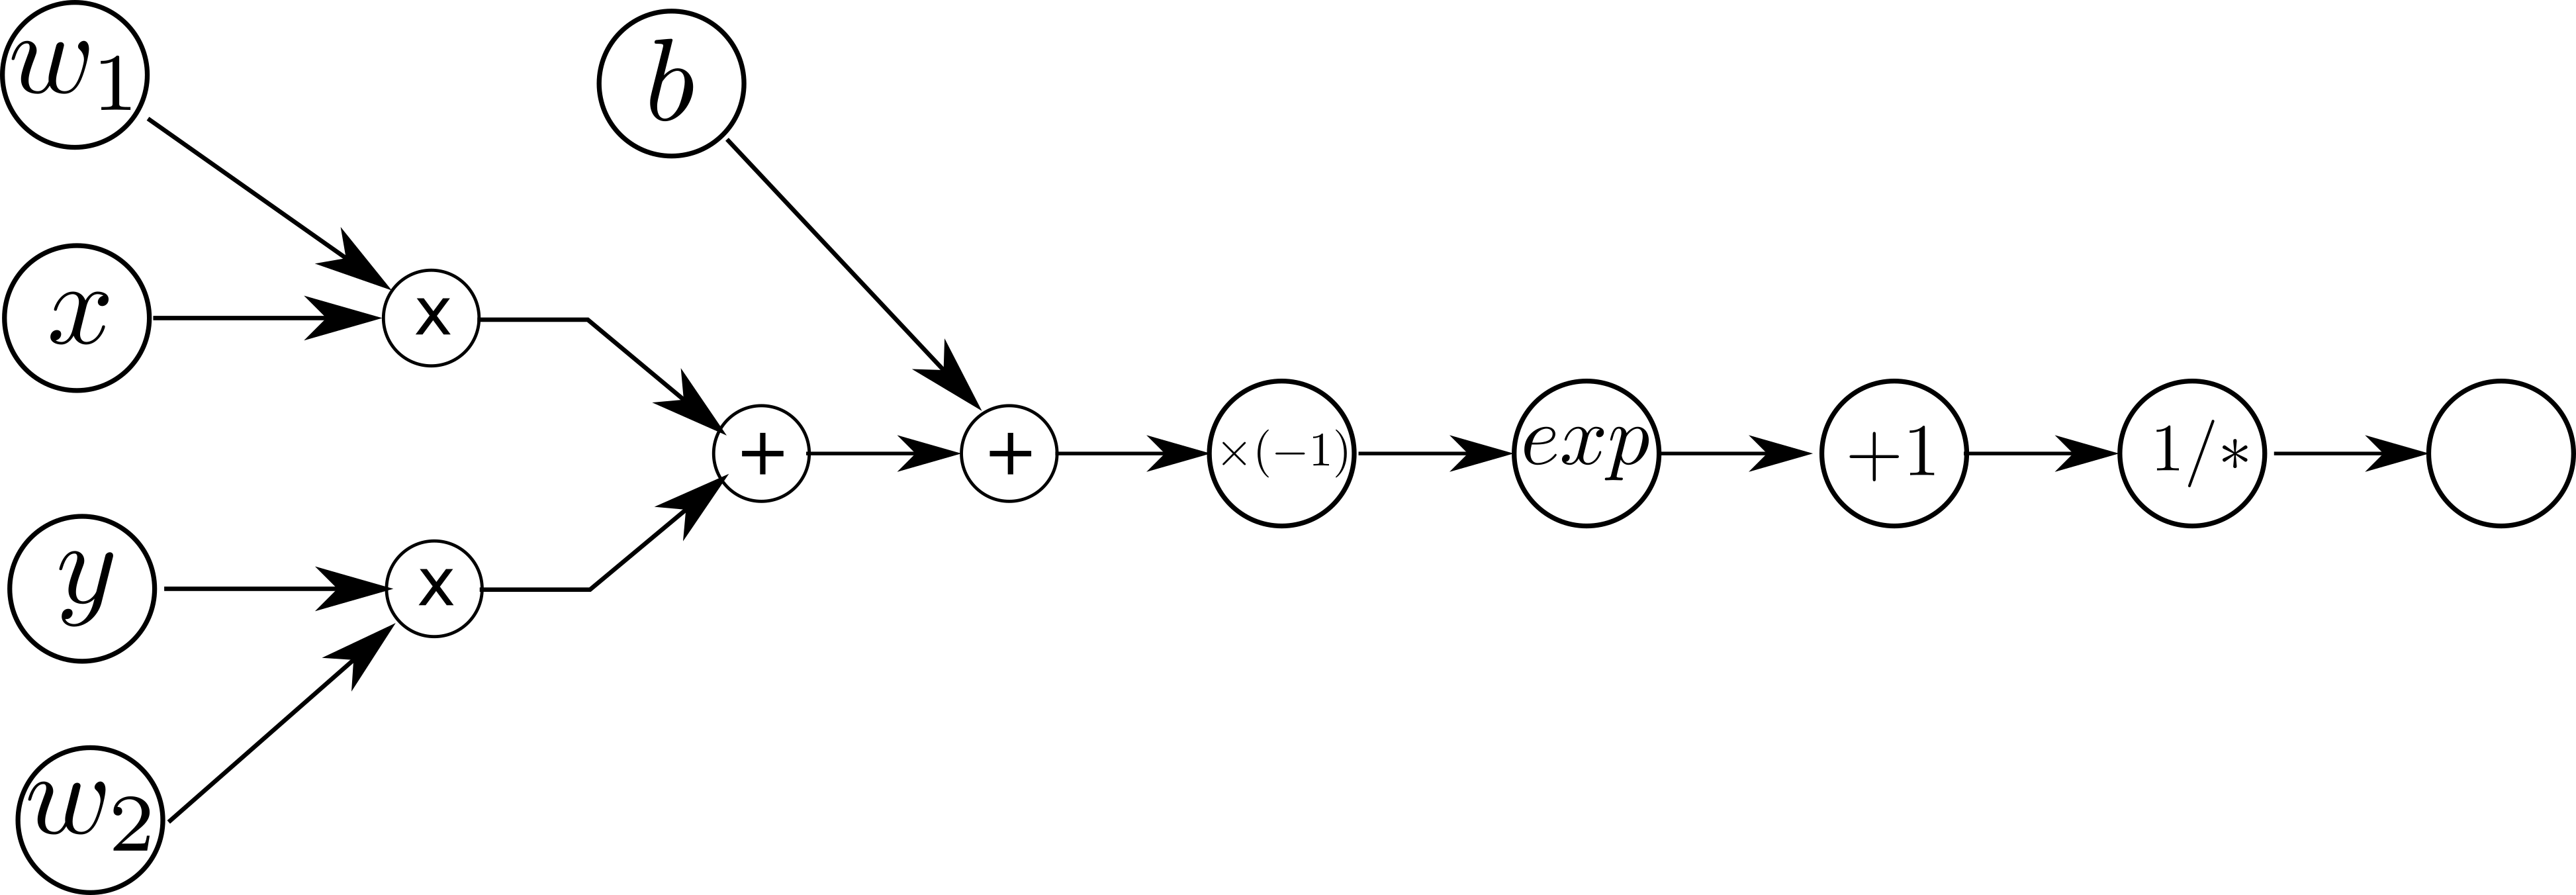
\includegraphics[width=0.6\textwidth]{comp_graph2}
\end{figure}

\begin{block}{Definition}
A computational graph is an acyclic directed graph such that:
\begin{itemize}
\item A node is a mathematical operator.
\item To each edge is associated a value.
\item Each node can compute the values of its output edges from the values of its input edges.
    \begin{itemize}
    \item Nodes without input edges are \emph{input nodes}. They represent the input values of the graph.
    \item Similarly, output values can be held in the \emph{output nodes}.
    \end{itemize}
\end{itemize}
\end{block}

\begin{figure}[h]
    \centering
    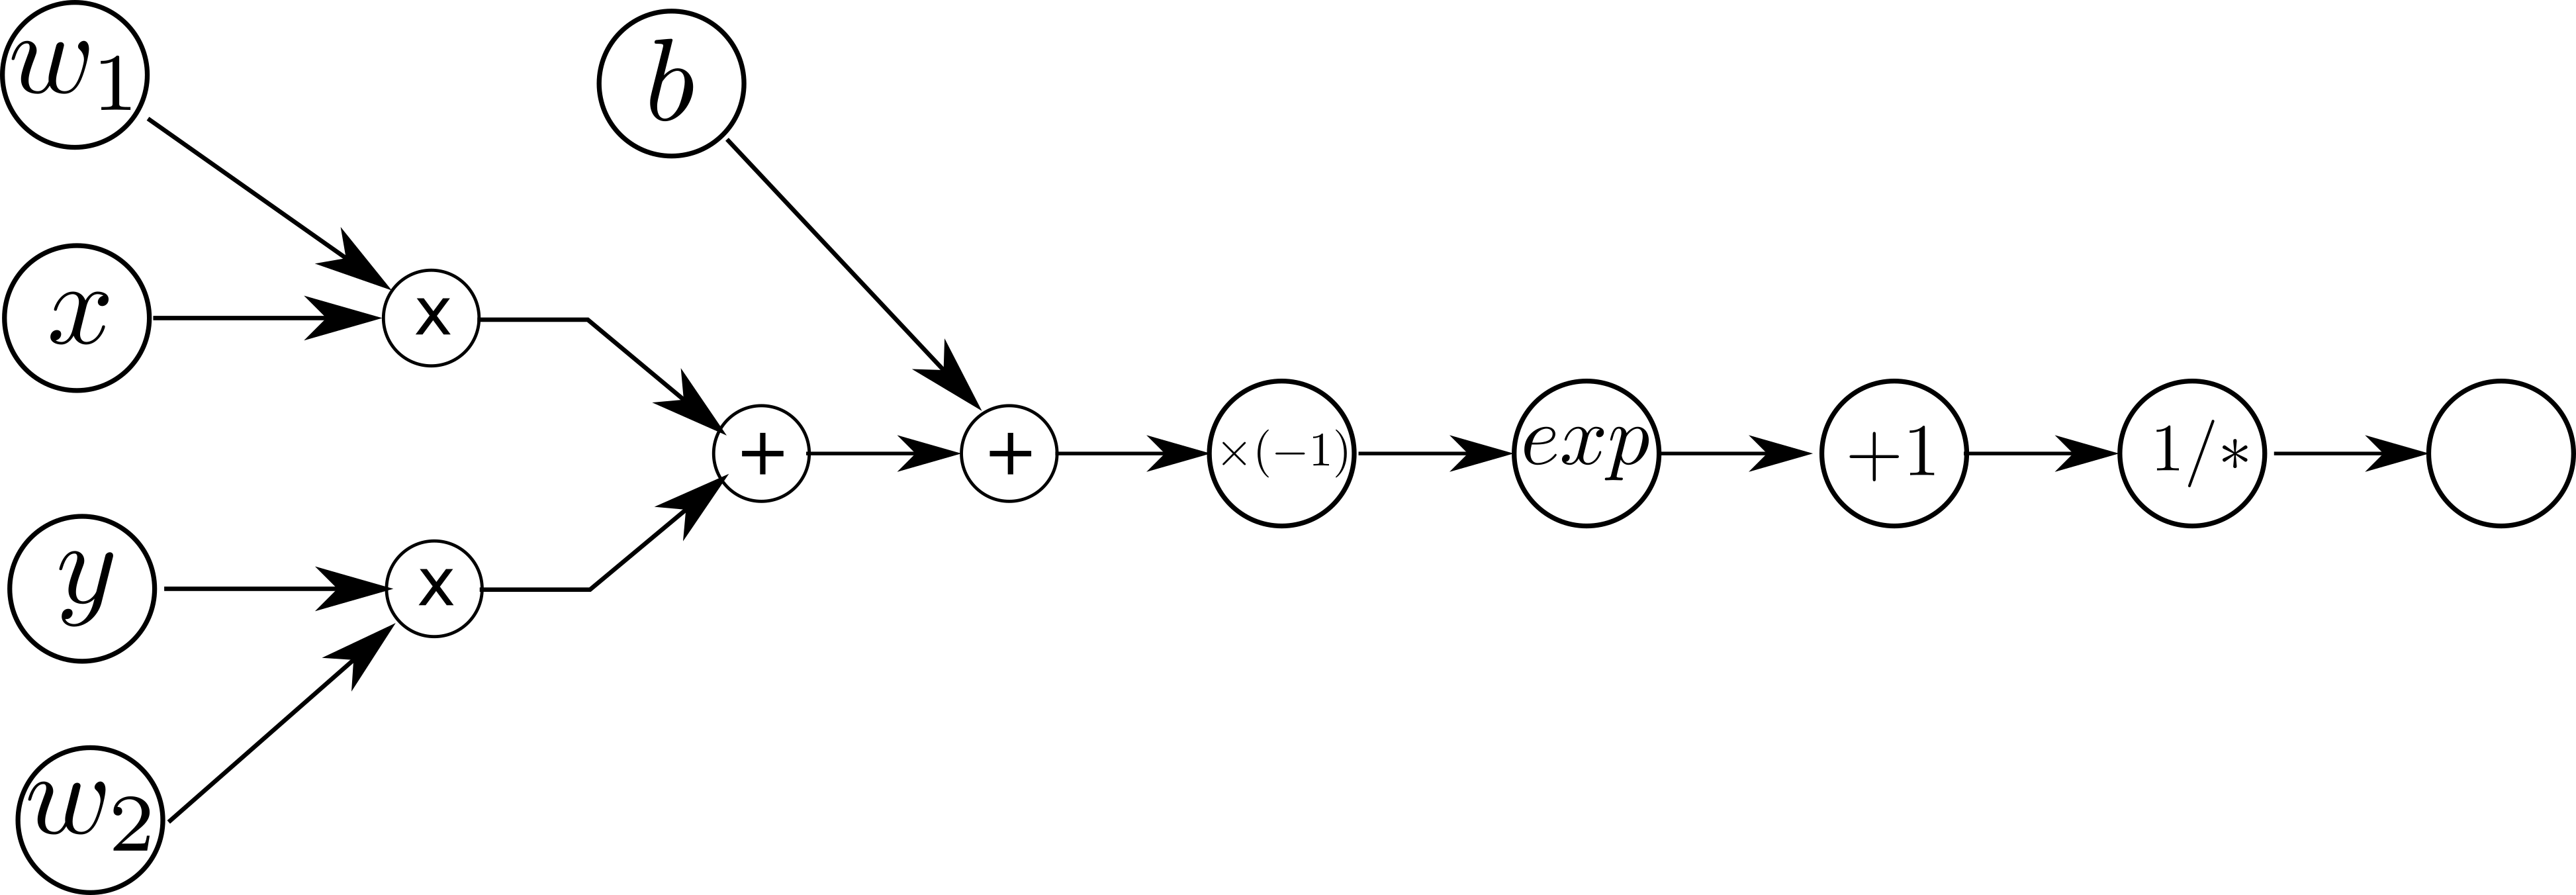
\includegraphics[width=0.6\textwidth]{comp_graph2}
\end{figure}

\begin{itemize}
\item In this course, we will only consider \emph{acyclic} computational graphs.
\item Computing a \emph{forward pass} through the graph means choosing its input values, and then progressively computing the values of all edges.
\end{itemize}

\section{Computational Graph Example}

Computational graph of:
\[
\sigma(w_1x + w_2y + b)
\]
where $\sigma$ is the sigmoid function: $\sigma(x) = \frac{1}{1 + e^{-x}}$

\begin{figure}[h]
    \centering
    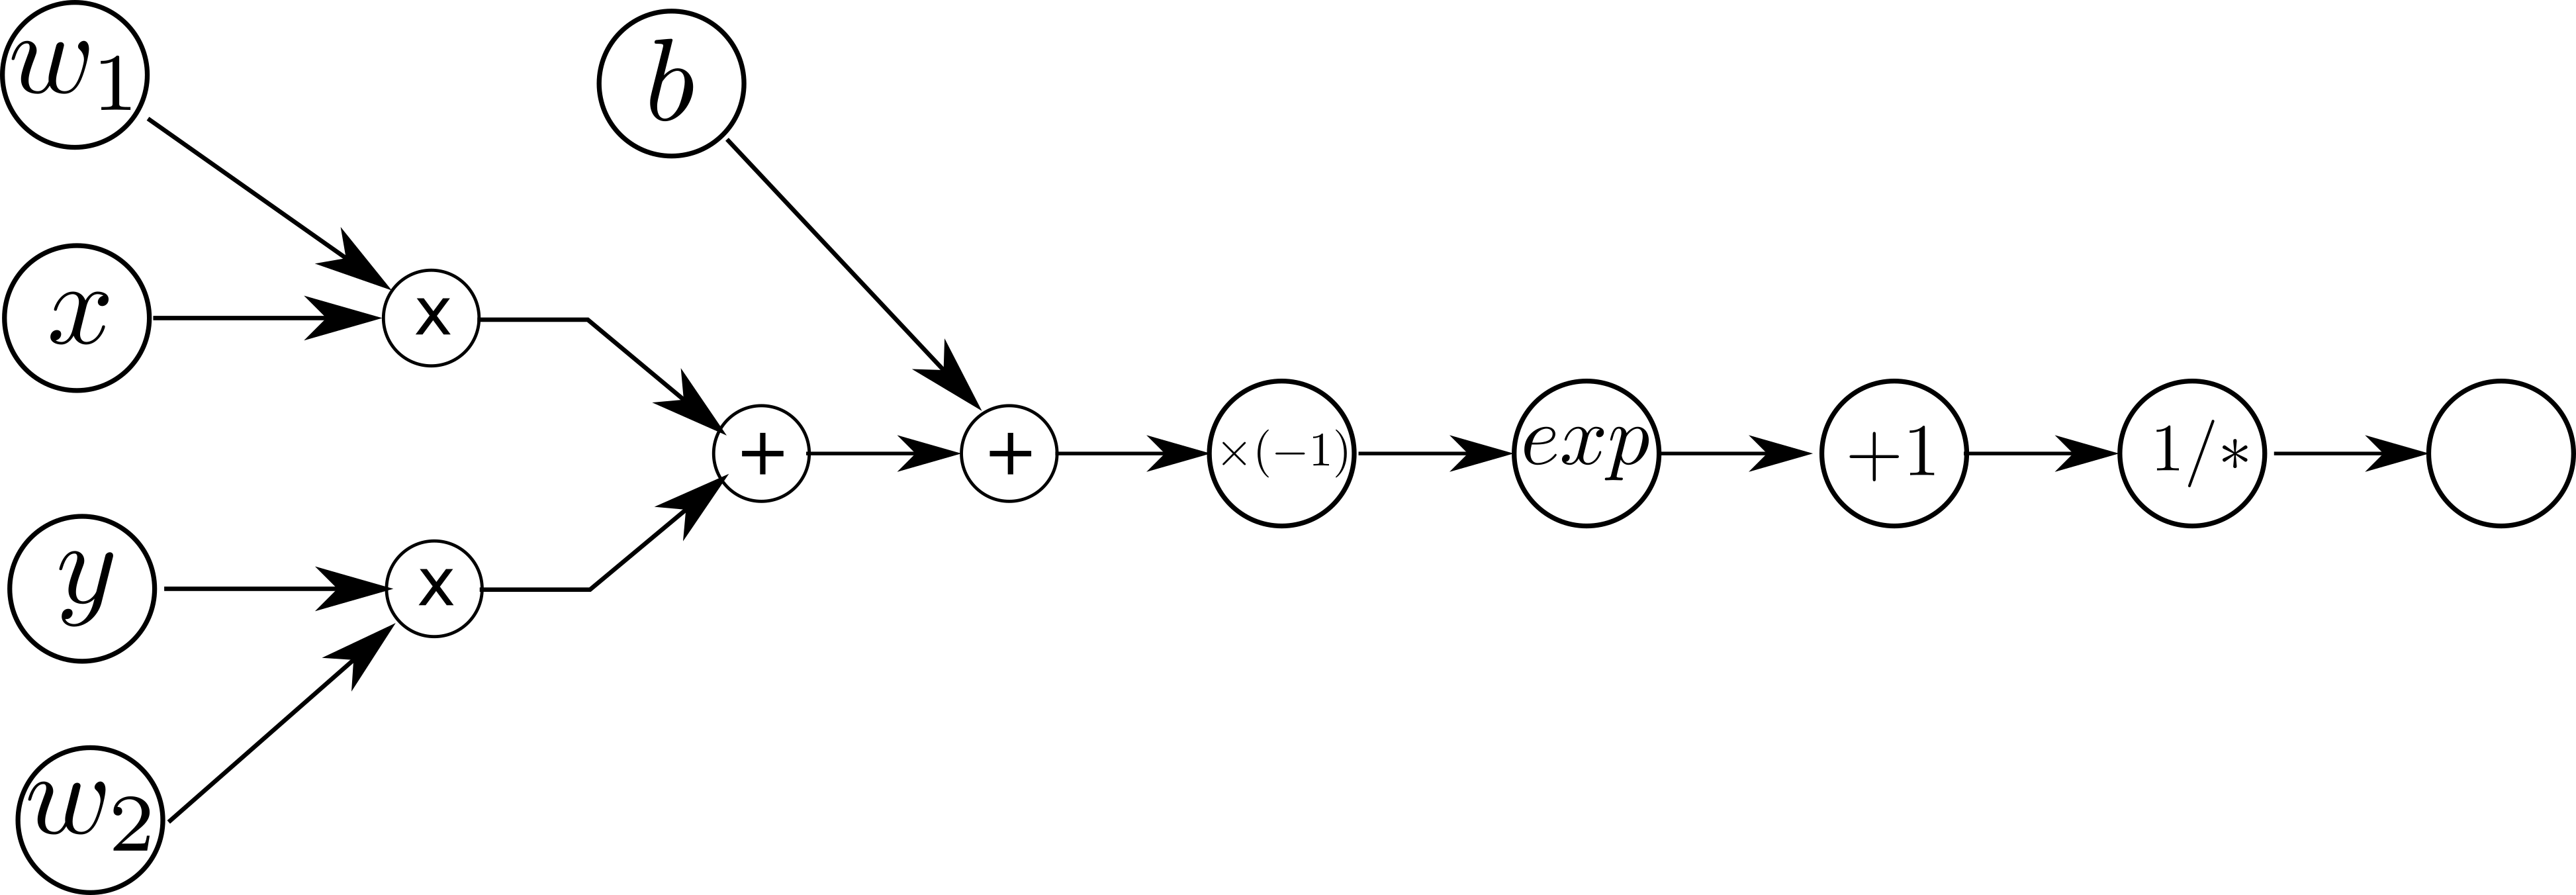
\includegraphics[width=0.6\textwidth]{comp_graph2}
\end{figure}

The graph can be represented at different levels of detail:
\begin{figure}[h]
    \centering
    \includegraphics[width=0.6\textwidth]{comp_graph}
\end{figure}

\section{First Architectures}

\subsection{Neural Network (NN)}

\begin{block}{Definitions}
\begin{itemize}
\item An artificial neural network is a computational graph, where the nodes are artificial neurons.
\item The \alert{input layer} is the set of neurons without incoming edges.
\item The \alert{output layer} is the set of neurons without outgoing edges.
\end{itemize}
\end{block}

\subsection{Network Layers}

\begin{block}{Definition}
\begin{itemize}
\item Neurons are usually organized in \alert{layers}.
\item Any layers other than input and output layers are called \alert{hidden layers}.
\end{itemize}
\end{block}

\begin{figure}[h]
    \centering
    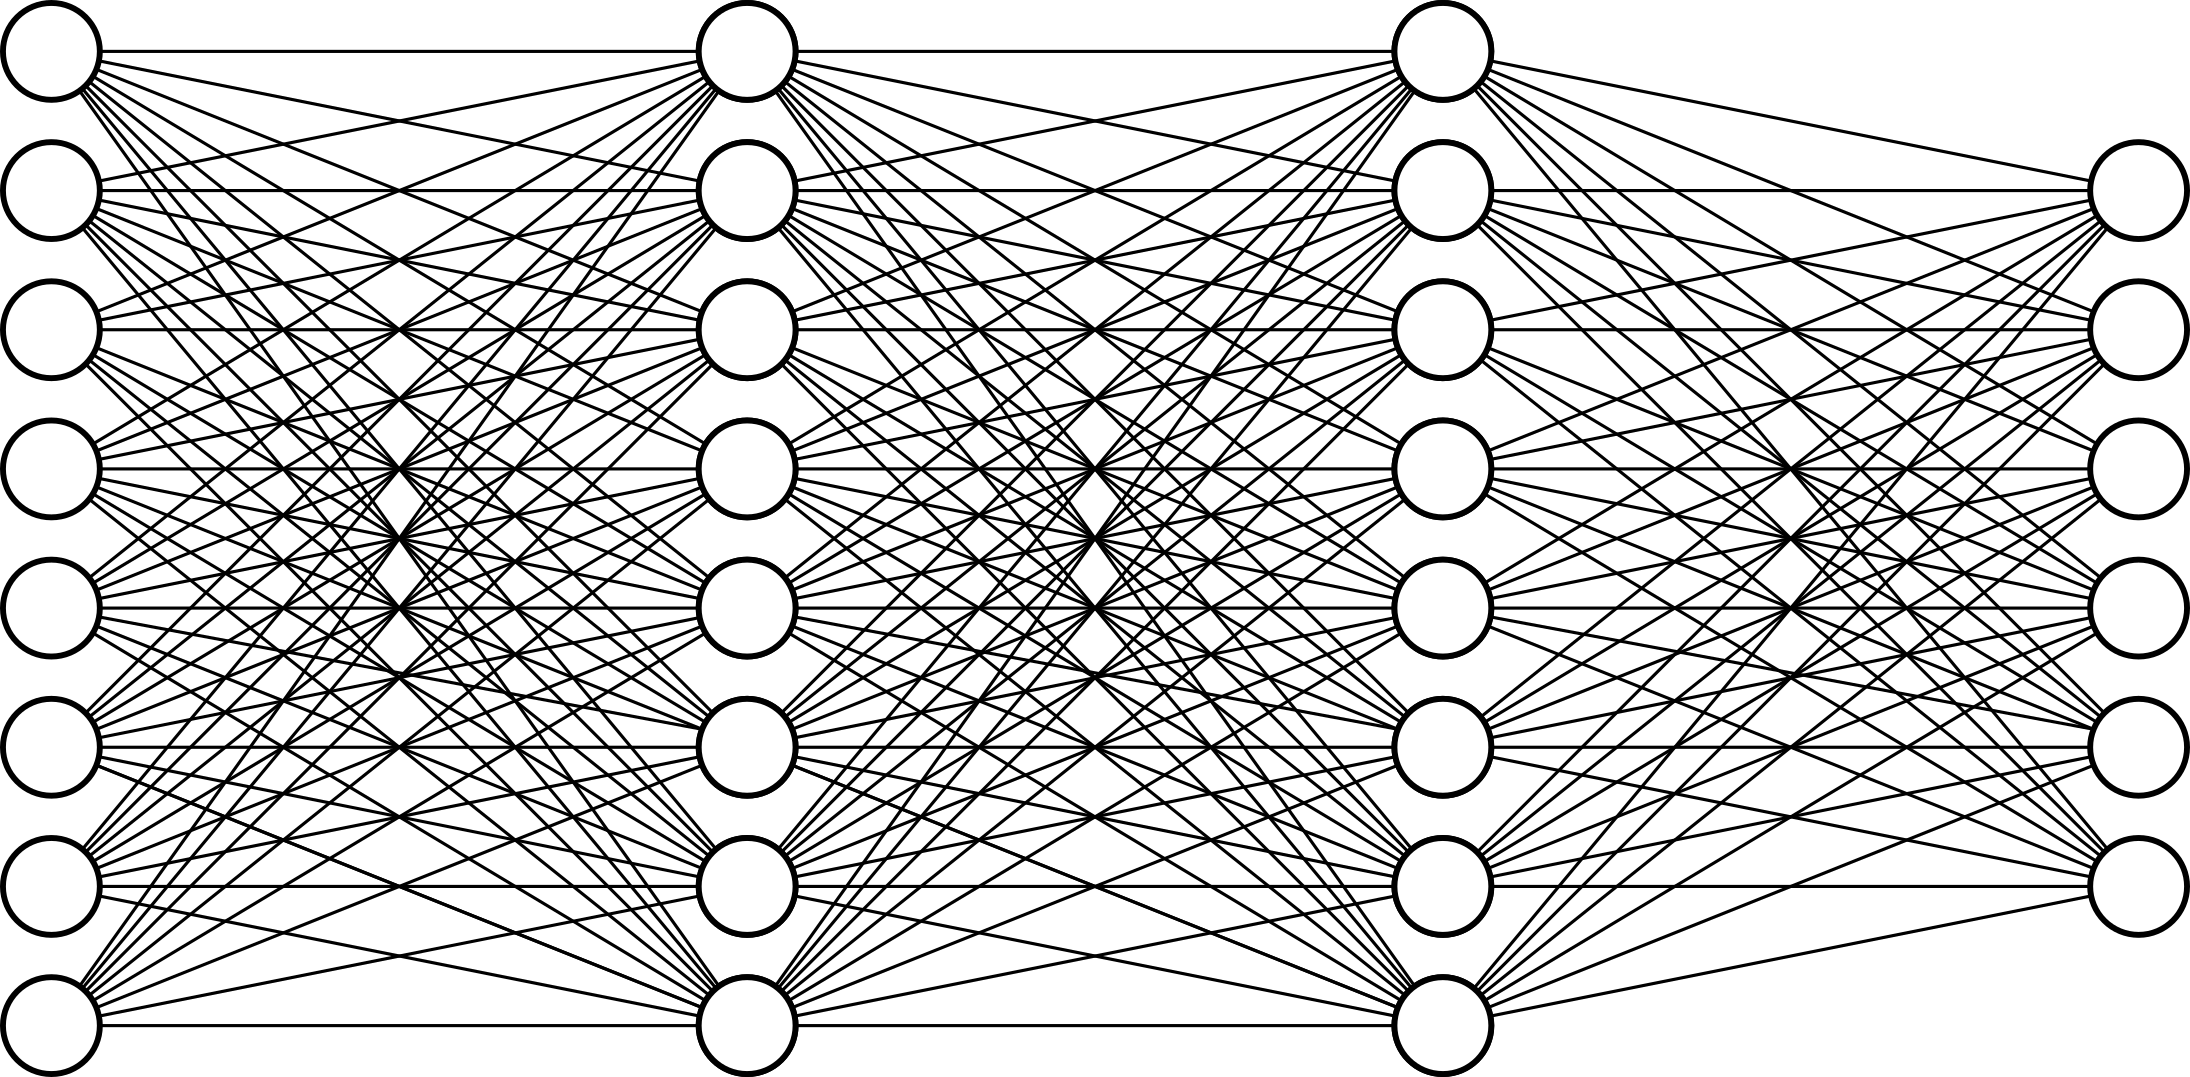
\includegraphics[height=3cm]{mini_reseau3_bis}
\end{figure}

\subsection{Other Types of Neural Networks}

\begin{block}{}
In the following of this course, except when otherwise specified, all NNs will be feed-forward. Indeed, this is the preferred type of NN for image processing.
\end{block}

\begin{block}{What about other architectures?}
\begin{itemize}
\item Recurrent neural networks (RNN).
\item Long short-term memory networks (LSTM).
\end{itemize}
\end{block}

\begin{itemize}
\item[+] More powerful than feed-forward NNs.
\item[-] Complex dynamics; more difficult to train.
\item Mainly used for processing temporal data.
\end{itemize}

\subsection{Fully-Connected Layer}

\begin{itemize}
\item A layer is said to be fully-connected (FC) if each of its neurons is connected to all the neurons of the previous layer.
\item If a FC layer contains $r$ neurons, and the previous layer $q$, then its weights are a 2D dimensional array (a matrix) of size $q \times r$.
\end{itemize}

\begin{figure}[h]
    \centering
    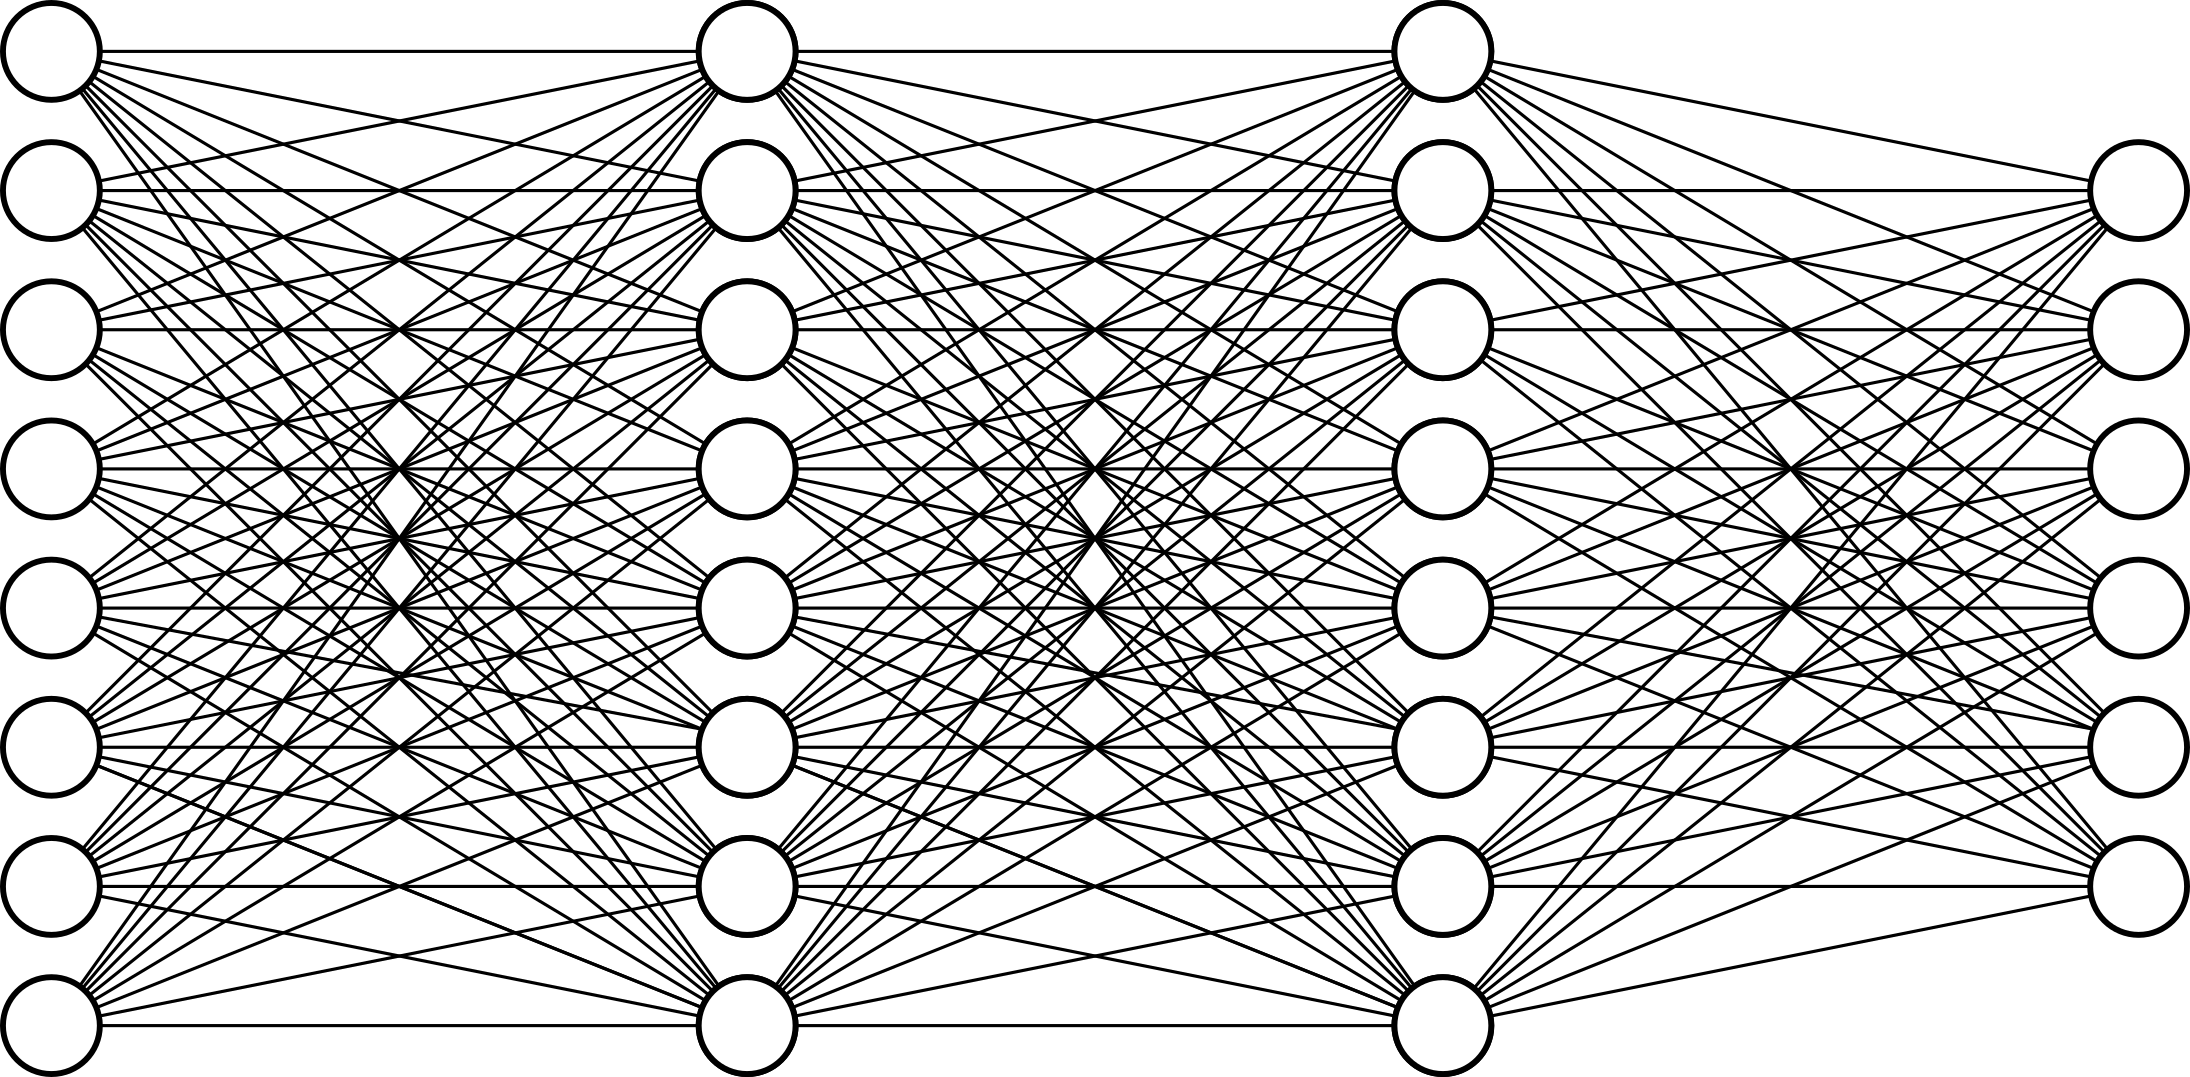
\includegraphics[height=3cm]{mini_reseau3_bis}
\end{figure}

\subsection{Graphical Representation of NNs}

\begin{figure}[h]
    \centering
    \begin{subfigure}{.5\textwidth}
        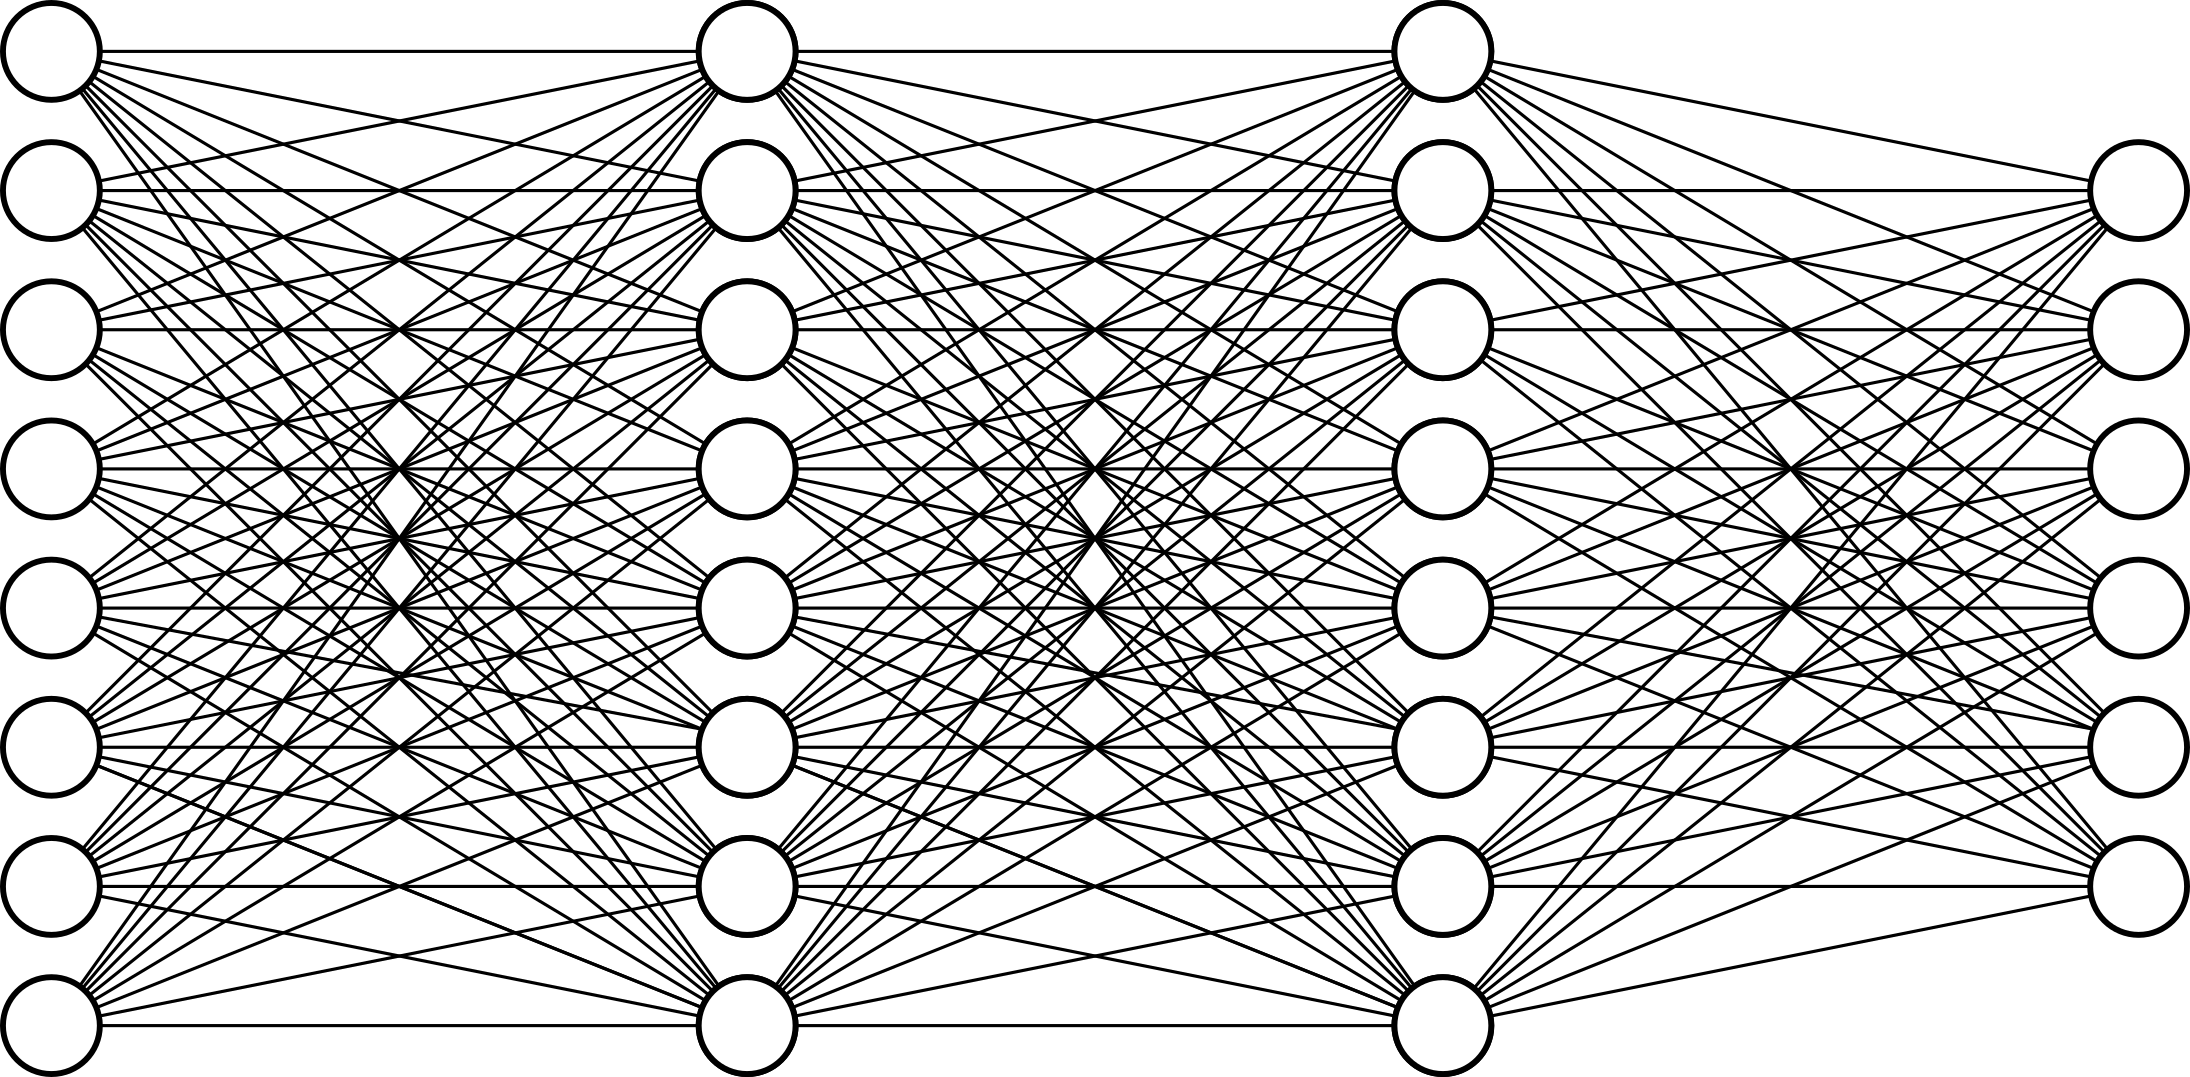
\includegraphics[height=3cm]{mini_reseau3_bis}
    \end{subfigure}
    \begin{subfigure}{.5\textwidth}
        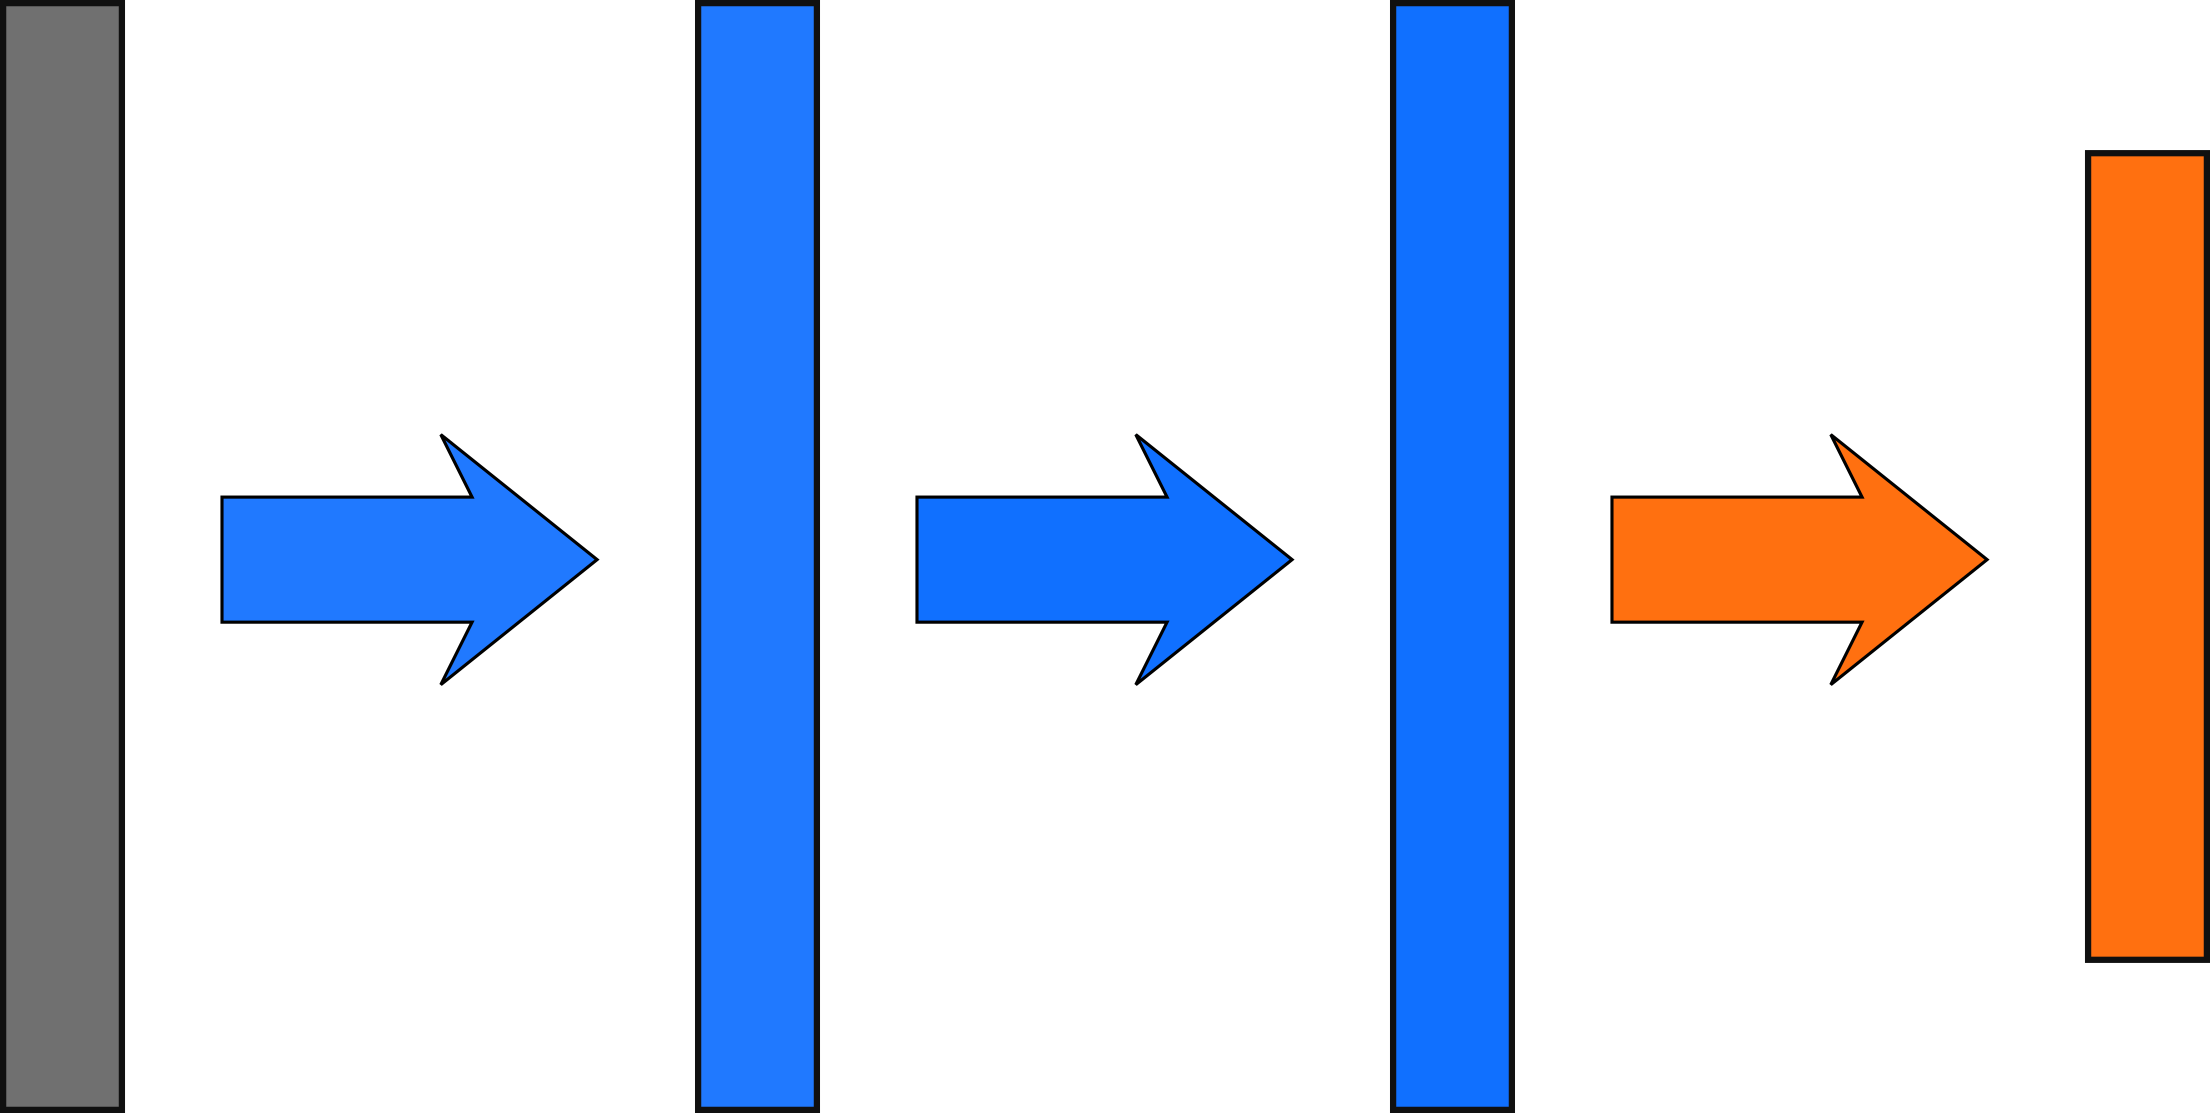
\includegraphics[height=3cm]{nn_representation3}
    \end{subfigure}
\end{figure}

\begin{itemize}
\item Data is organized into arrays, linked with operators.
\item A layer corresponds to an operator between arrays.
\end{itemize}

\subsection{The Equations of a Fully Connected Neural Network}

\begin{figure}[h]
    \centering
    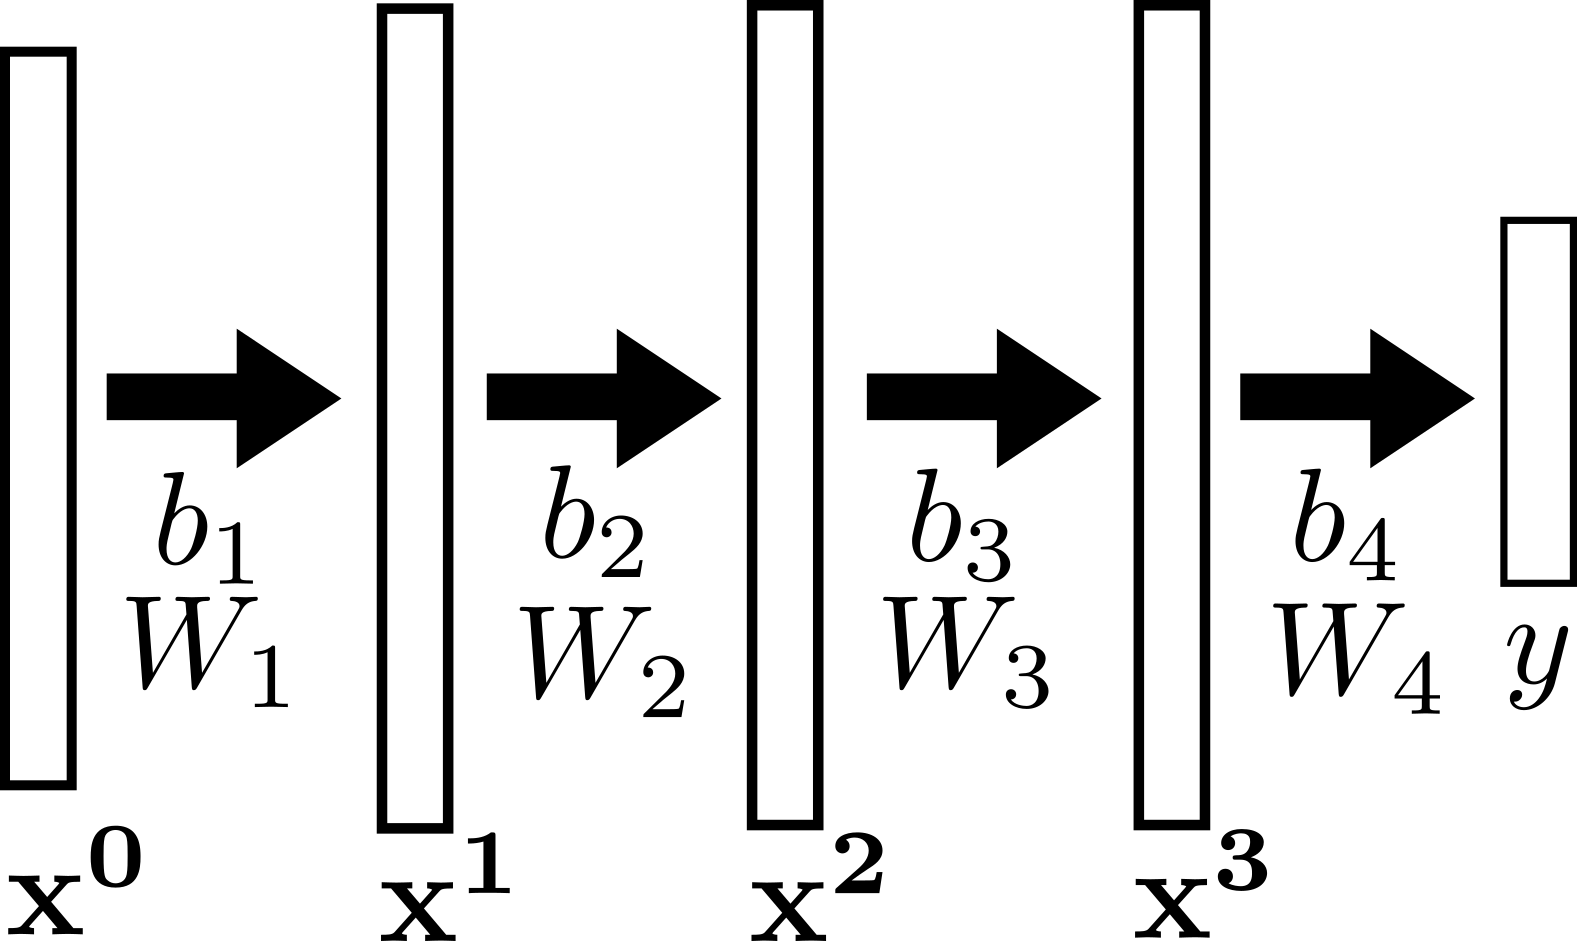
\includegraphics[height=3cm]{nn_representation2}
\end{figure}

\begin{block}{}
For $i \in \{1, 2, 3\}$:
\[
\x_i = \act_i(\x_{i-1}^t \W_i + \bias_i)
\]
\end{block}

\begin{block}{}
\[
\y = \act_4(\x_4^t \W_4 + \bias_4)
\]
\end{block}

What would happen if all activation functions $\act_i$ were equal to the identity function?

\subsection{Number of Parameters}

\begin{figure}[h]
    \centering
    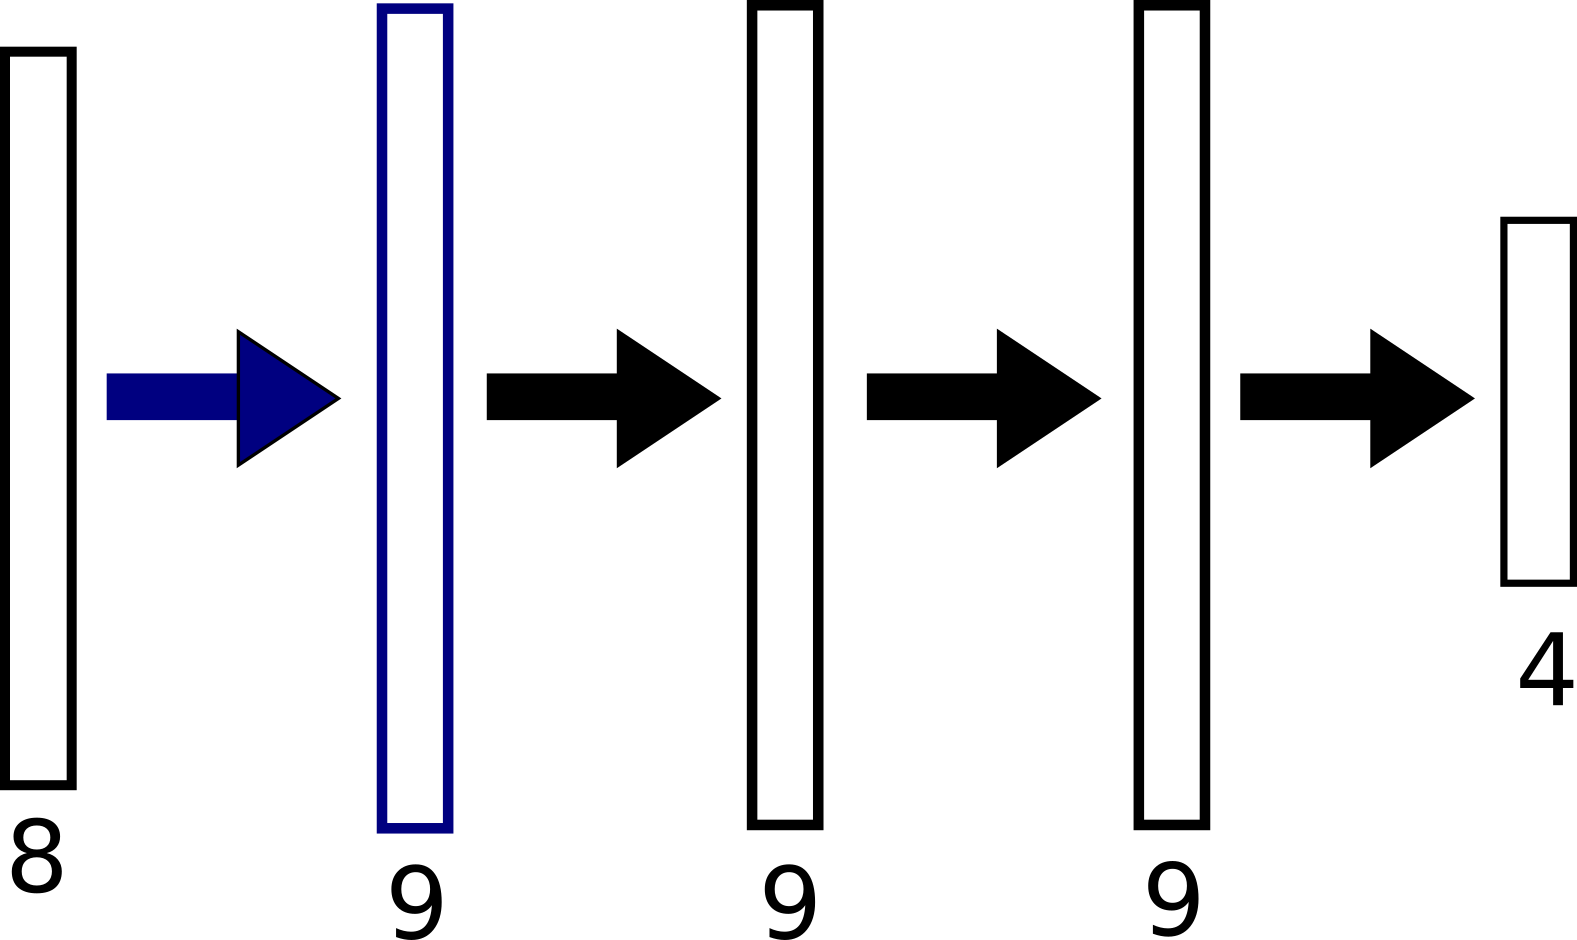
\includegraphics[height=3cm]{nn_representation.png}
\end{figure}

\begin{itemize}
\item How many parameters does the above network contain?
\end{itemize}

\begin{itemize}
\item[A/] 270
\item[B/] 274
\item[C/] 301
\item[D/] 39
\end{itemize}

\subsection{Batch Processing}

In a learning context, one may want to process $n$ vectors of length $p$ at the same time. They can be grouped into a matrix $\mathbf{X}$ of size $n \times p$. The $n$ corresponding outputs $\y_i$ can also be grouped into a matrix $\Y$. The resulting equations are:

\begin{block}{}
For $i \in \{1, 2, 3\}$:
\[
\X_i = \act_i(\X_{i-1}\W_i + \bias_i)
\]
\end{block}

\begin{block}{}
\[
\Y = \act_4(\X_4\W_4 + \bias_4)
\]
\end{block}

This can accelerate processing thanks to hardware architectures such as Graphical Processing Units (GPUs) but can also play an important role in optimization.

\subsection{From Neurons to Arrays}

\begin{itemize}
\item Neurons are organized into arrays (0-D, 1-D, 2-D, 3-D ...).
\item Artificial neural networks can be seen as \textcolor{blue}{computational graphs processing arrays}.
\end{itemize}

\section{Modelling Power}

\subsection{A Composition of Differentiable Functions}

\begin{itemize}
\item The functions composing an artificial neural network are differentiable (almost everywhere), so that it can be optimized via gradient descent. Therefore, an ANN is differentiable (almost everywhere).
\item In fact, any continuous function on a closed bounded domain can be approached within any error margin by an artificial neural network.
\end{itemize}

\subsection{Universal Approximation Theorem}

\begin{figure}[h]
    \centering
    \begin{subfigure}{.5\textwidth}
        \begin{itemize}
        \item We have previously seen that a neuron can be used as a linear classifier and that combining several of them one can build complex classifiers.
        \item We will see that this observation can be generalized.
        \end{itemize}
    \end{subfigure}
    \begin{subfigure}{.5\textwidth}
        \includegraphics[height=4cm]{circles_H}
    \end{subfigure}
\end{figure}

\begin{block}{}
Let $f$ be a \textcolor{blue}{continuous} real-valued function of $[0,1]^p$ ($p \in \N^*$) and $\epsilon$ a strictly positive real. Let $\act$ be a non-constant, increasing, bounded real function (\emph{\small{the activation function}}).

Then there exists an integer $q$, real vectors $\{\mathbf{w}_i\}_{1 \leq i \leq q}$ of $\R^p$, and reals $\{b_i\}_{1 \leq i \leq q}$ and $\{v_i\}_{1 \leq i \leq q}$ such that for all $\x$ in $[0,1]^p$:

\[
\left| f(\x) - \sum\limits_{i=1}^q v_i \act(\mathbf{w}_i\x + b_i) \right| < \epsilon
\]
\end{block}

A first version of this theorem, using sigmoidal activation functions, was proposed by \cite{cybenko_approximations_1989}. The version above was demonstrated by \cite{hornik_approximation_1991}.

\subsection{Universal Approximation Theorem: What Does It Mean?}

\[
\left| f(\x) - \sum\limits_{i=1}^q v_i \act(\mathbf{w}_i\x + b_i) \right| < \epsilon
\]

This means that function $f$ can be approximated with a neural network containing:
\begin{itemize}
\item An input layer of size $p$.
\item A hidden layer containing $q$ neurons with activation function $\act$, weights $\mathbf{w}_i$ and biases $b_i$.
\item An output layer containing a single neuron, with weights $v_i$ (and an identity activation function).
\end{itemize}

\subsection{Universal Approximation Theorem in Practice}

\begin{itemize}
\item The number of neurons increases very rapidly with the complexity of the function.
\item Empirical evidence has shown that \alert{multi-layer architectures give better results}.
\item For learning tasks, the function to be modelled is only known on a finite number of points.
\end{itemize}

\begin{block}{}
A NN can potentially have a lot of parameters. How can we set them?
\end{block}

\chapter{Training a Neural Network}

\section{Introduction}

\begin{itemize}
\item We have seen that NNs have a lot of potential. However, how can the parameters $\param = (\W_i, \bias_i)$ be set?
\item What is our objective?
\end{itemize}

\section{Supervised Learning Problem}

We recall that our training set contains $n$ samples:

\[
(\x_i, y_i) \in \R^p \times \mathcal{Y}
\]

Where $\mathcal{Y}=\R$ in the regression case and $\mathcal{Y}=\{0, 1\}$ in the binary classification case.

We \textcolor{blue}{choose} a loss function $l$ and we \textcolor{blue}{choose} a family $f_{\param}$ of functions from $\R^p$ into $\R$, depending on a set of parameters $\param$, and \textcolor{blue}{find} the value $\param^{\ast}$ of $\param$ that minimizes:

\[
\frac{1}{n} \sum\limits_{i=1}^{n} l (f_{\param}(\x_i), y_i)
\]

\vspace{1em}

\small{For the sake of simplicity, we have dropped the regularization term.}

\section{Loss Functions}

\subsection{Choosing a Loss Function}

\begin{itemize}
\item The choice of the loss function depends on the type of problem (regression or classification) and is tightly linked to the application.
\end{itemize}

\subsection{The Standard Loss for Regression Problems: Squared Error Loss}

In the regression case, we have $\mathcal{Y} = \R$.

\begin{block}{Squared Error Loss}
\[
l(f_{\param}(x), y) = (f_{\param}(x) - y)^2
\]
\end{block}

\subsection{Binary Cross-Entropy}

In the simplest classification case, we have $\mathcal{Y}=\{0, 1\}$.

\begin{block}{Binary Cross-Entropy Loss}
\[
l(f_{\param}(x), y) = - y \log(f_{\param}(x)) - (1 - y) \log(1 - f_{\param}(x))
\]
\end{block}

\begin{itemize}
\item For this expression to be mathematically sound, $f_{\param}(x)$ must belong to $]0, 1[$. In practice, in the case of NN, this can be achieved by using a sigmoid as last activation.
\item Note that the expression above is equivalent to:
\end{itemize}

\[
l(f_{\param}(x), y) = \left\{
\begin{array}{ll}
- \log(1 - f_{\param}(x)) & \mbox{if } y=0 \\
- \log(f_{\param}(x)) & \mbox{if } y=1
\end{array}
\right.
\]

\section{How to Minimize the Loss?}

\begin{figure}[h]
    \centering
    \begin{subfigure}{.6\textwidth}
        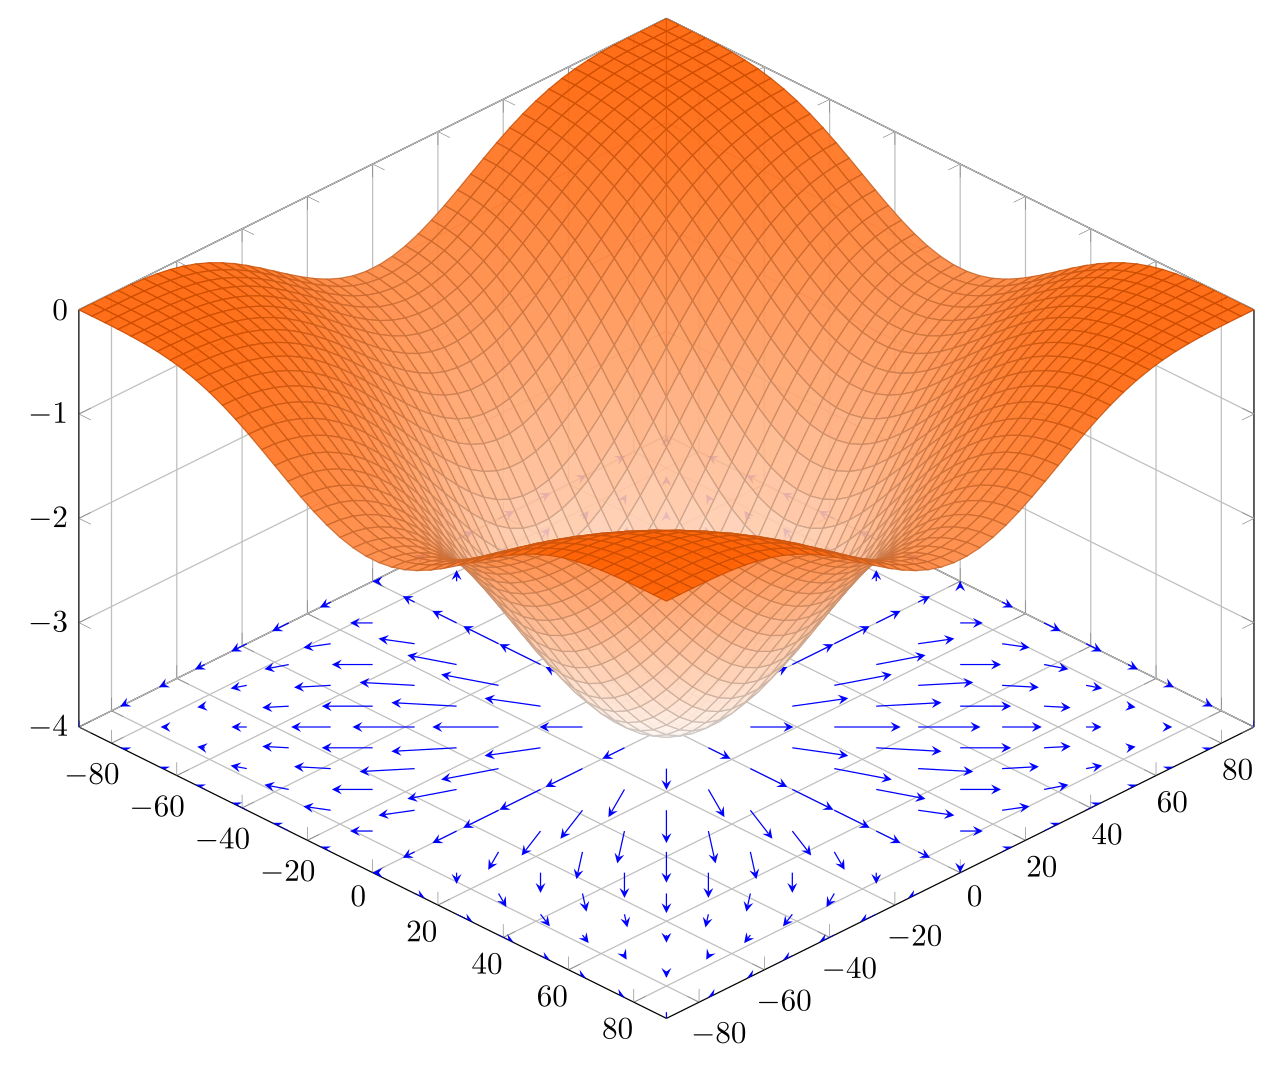
\includegraphics[height=5cm]{3d-gradient-cos.png}
    \end{subfigure}
    \begin{subfigure}{.4\textwidth}
        \begin{block}{Definition: Gradient}
        Let $\loss$ be a differentiable function from $\R^n$ into $\R$. Its gradient $\nabla\loss$ is:
        \[
        \nabla \loss (x) =
        \begin{pmatrix}
        \frac{\partial \loss}{\partial \x_1}(x) \\
        \vdots \\
        \frac{\partial \loss}{\partial \x_n}(x)
        \end{pmatrix}
        \]
        \end{block}
    \end{subfigure}
\end{figure}

\section{Gradient Descent}

\subsection{Gradient Descent in the Scalar Case}

\begin{figure}[h]
    \centering
    \begin{subfigure}{.5\textwidth}
        \includegraphics[width=\textwidth]{gradient_descent}
    \end{subfigure}
    \begin{subfigure}{.5\textwidth}
        \[
        \param_{t+1} = \param_t - \lr\nabla \loss(\param_t)
        \]
        $\loss$ is called the \alert{learning rate}.
    \end{subfigure}
\end{figure}

\subsection{Gradient Descent}

\begin{block}{Definition}
Gradient descent is an optimization algorithm. For a differentiable function $\loss$, a positive real $\lr$ (the \alert{learning rate}) and a starting point $\param_0$, it computes a sequence of values:
\[
\forall t \in \N: \param_{t+1} = \param_t - \lr \nabla \loss(\param_t)
\]
\end{block}

\begin{block}{Property}
For a given $t$, if $\lr$ is small enough, then:
\[
\loss(\param_{t+1}) \leq \loss(\param_t)
\]
\end{block}

Gradient descent is an essential tool in optimization.

\subsection{Gradient Descent: Stopping Criteria}

In practice:
\[
\forall t \in [0, \ldots, E-1]:\quad \param_{t+1} = \param_t - \lr \nabla \loss(\param_t)
\]

\begin{itemize}
\item Choose $E$ (the number of \alert{epochs}) based on experience.
\item Track the quality of the model using a validation dataset and stop when the validation loss does not improve.
\end{itemize}

\subsection{Towards Stochastic Gradient Descent}

The loss function we initially defined depends on the whole training set:
\[
\loss(\param) = \frac{1}{n} \sum\limits_{i=1}^n l(y_i, f_{\param}(\x_i))
\]

\begin{itemize}
\item If $n$ is very large, computing $\loss$ is impractical.
\item A computation on the whole training set leads to a single update of the model parameters - convergence can therefore be slow.
\end{itemize}

\subsection{Stochastic Gradient Descent}

In \alert{stochastic gradient descent}, the parameters are updated for each sample $i$.

\begin{itemize}
\item First, the loss is computed
\[
\loss(\param_t) = l(y_i, f(\x_i, \param_t))
\]
\item The gradient $\nabla \loss(\param_t)$ is computed and
\item Finally the parameters are updated:
\[
\param_{t+1} = \param_t - \lr\nabla \loss(\param_t)
\]
\item Note that the learning rate $\lr$ can have a different value than in classic gradient descent.
\end{itemize}

\subsection{Mini-Batch Processing}

\begin{itemize}
\item One can (and often does) choose an intermediate solution between the full gradient and the stochastic gradient: mini-batch gradient.
\item The training database is then separated into subsets containing $m$ samples ($m < n$).
\item This has a regularization effect on the optimization with respect to the stochastic gradient and speeds up computation thanks to the vectorization capacity of hardware architectures such as GPUs.
\end{itemize}

\section{Backpropagation}

\subsection{Gradient Descent Applied to Neural Networks}

\begin{figure}[h]
    \centering
    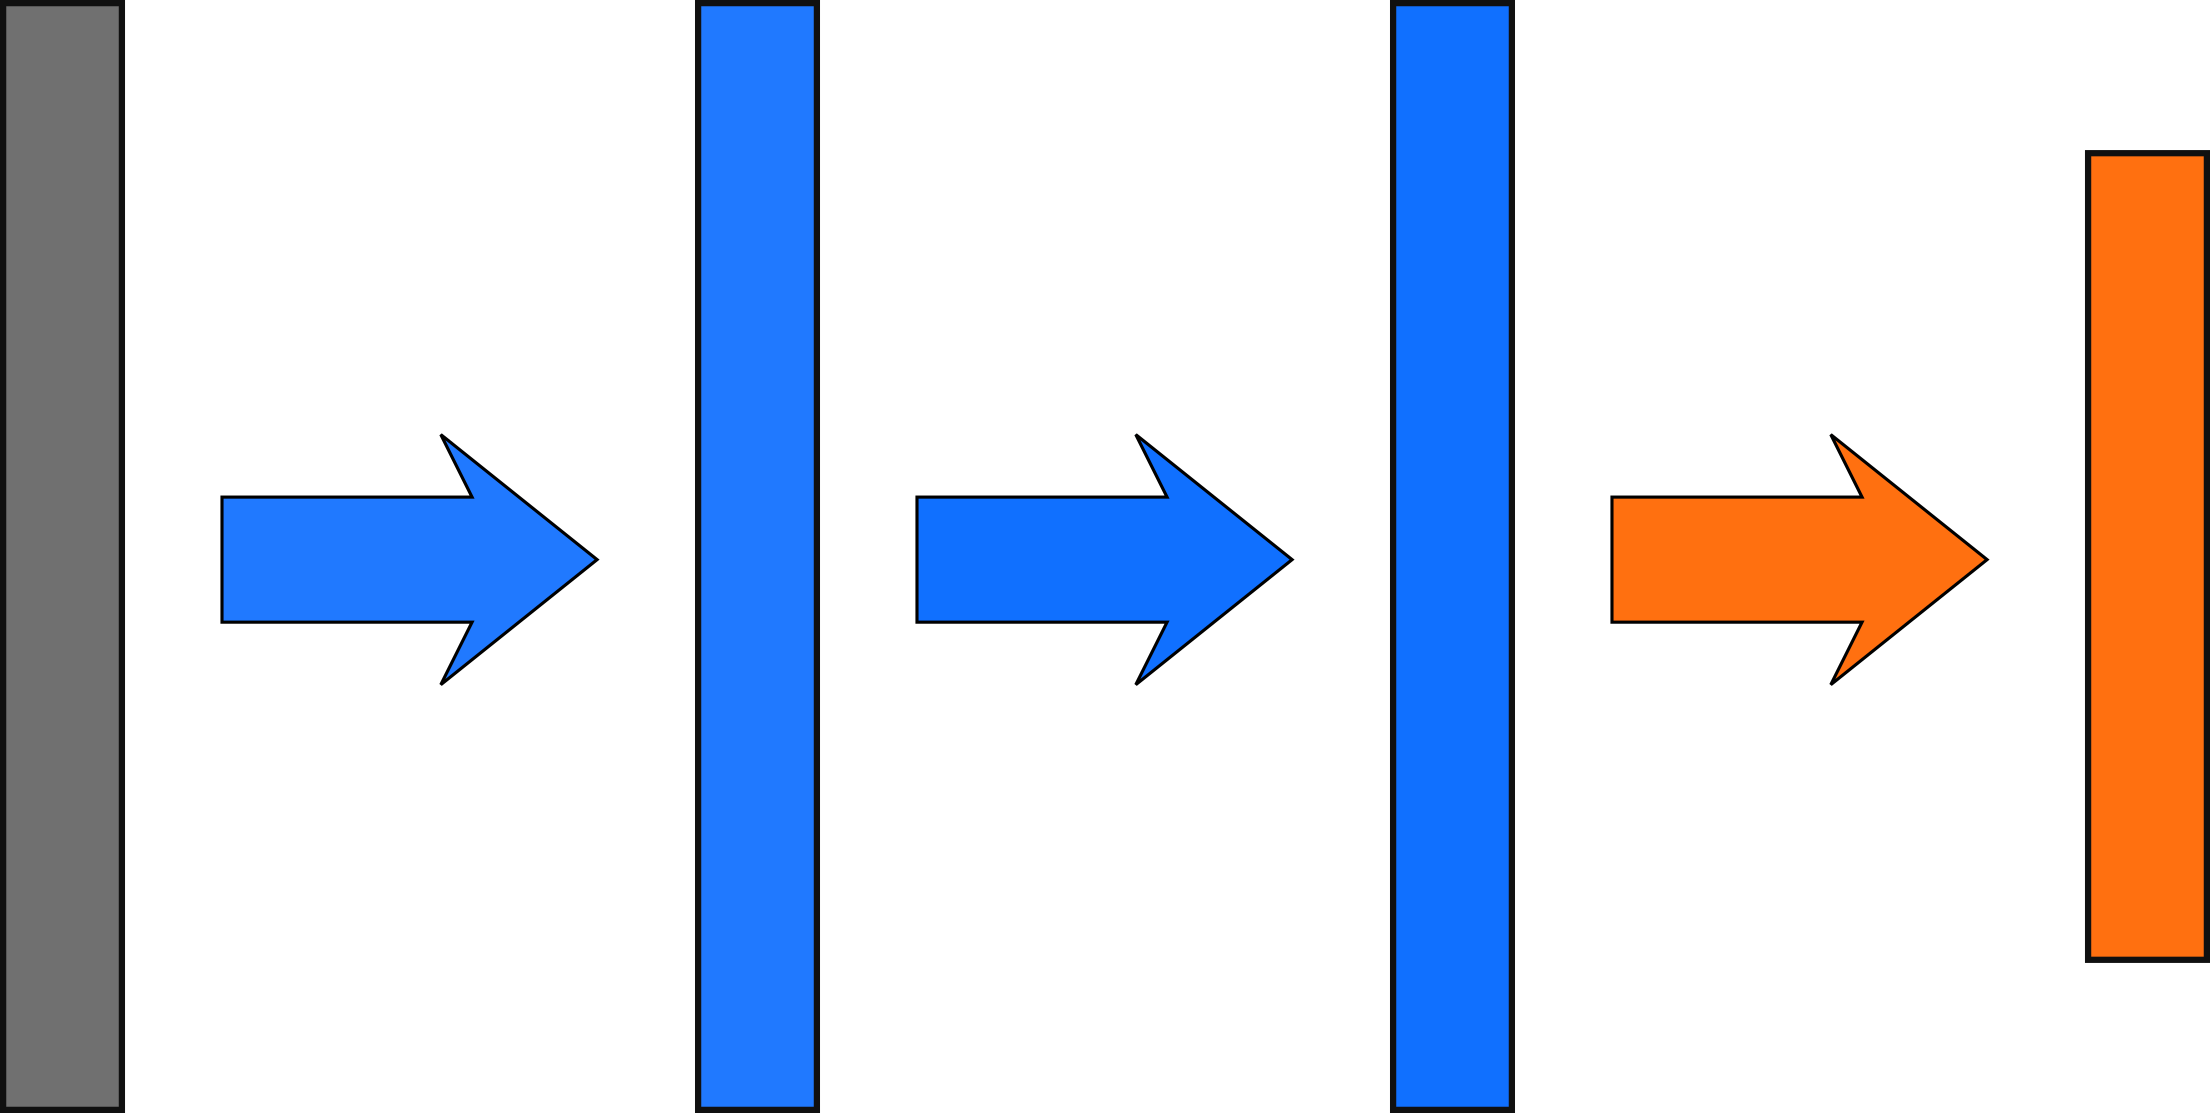
\includegraphics[height=3cm]{nn_representation3}
\end{figure}

\begin{itemize}
\item In the case of neural networks, the loss $\loss$ depends on each parameter $\param_i$ via the composition of several functions.
\item Analytical derivation is possible, but complex - and has to be re-computed when the network architecture is modified.
\item Using the chain rule theorem leads to an efficient solution: \textcolor{blue}{backpropagation}.
\end{itemize}

\subsection{Chain Rule Theorem}

\begin{block}{}
Let $f_1$ and $f_2$ be two differentiable real functions ($\R \rightarrow \R$). Then for all $x$ in $\R$:
\[
(f_2 \circ f_1)'(x) = (f_2'\circ f_1)(x).f_1'(x)
\]
\end{block}

\begin{block}{Leibniz Notation}
Let us introduce variables $x$, $y$ and $z$:
\[x \xrightarrow{f_1} y \xrightarrow{f_2} z\]

Then:
\[\dv{z}{x} = \dv{z}{y} \cdot \dv{y}{x} \]
\end{block}

\subsection{The Backpropagation Algorithm}

\begin{itemize}
\item The backpropagation algorithm is used in a neural network to efficiently compute the partial derivatives of the loss with respect to each parameter of the network.
\item One can trace the origins of the method to the sixties.
\item It was first applied to NN in the eighties \cite{werbos_applications_1982, lecun_procedure_1985}.
\end{itemize}

\subsection{The Backpropagation Algorithm: Intuition}

\begin{itemize}
\item Given a computational graph, the main idea is to compute the local derivatives during a forward pass.
\item Then, during a backward pass, the partial derivatives of the loss with respect to each parameter are computed.
\end{itemize}

\subsection{Simple Backpropagation Example}

\begin{figure}[h]
    \centering
    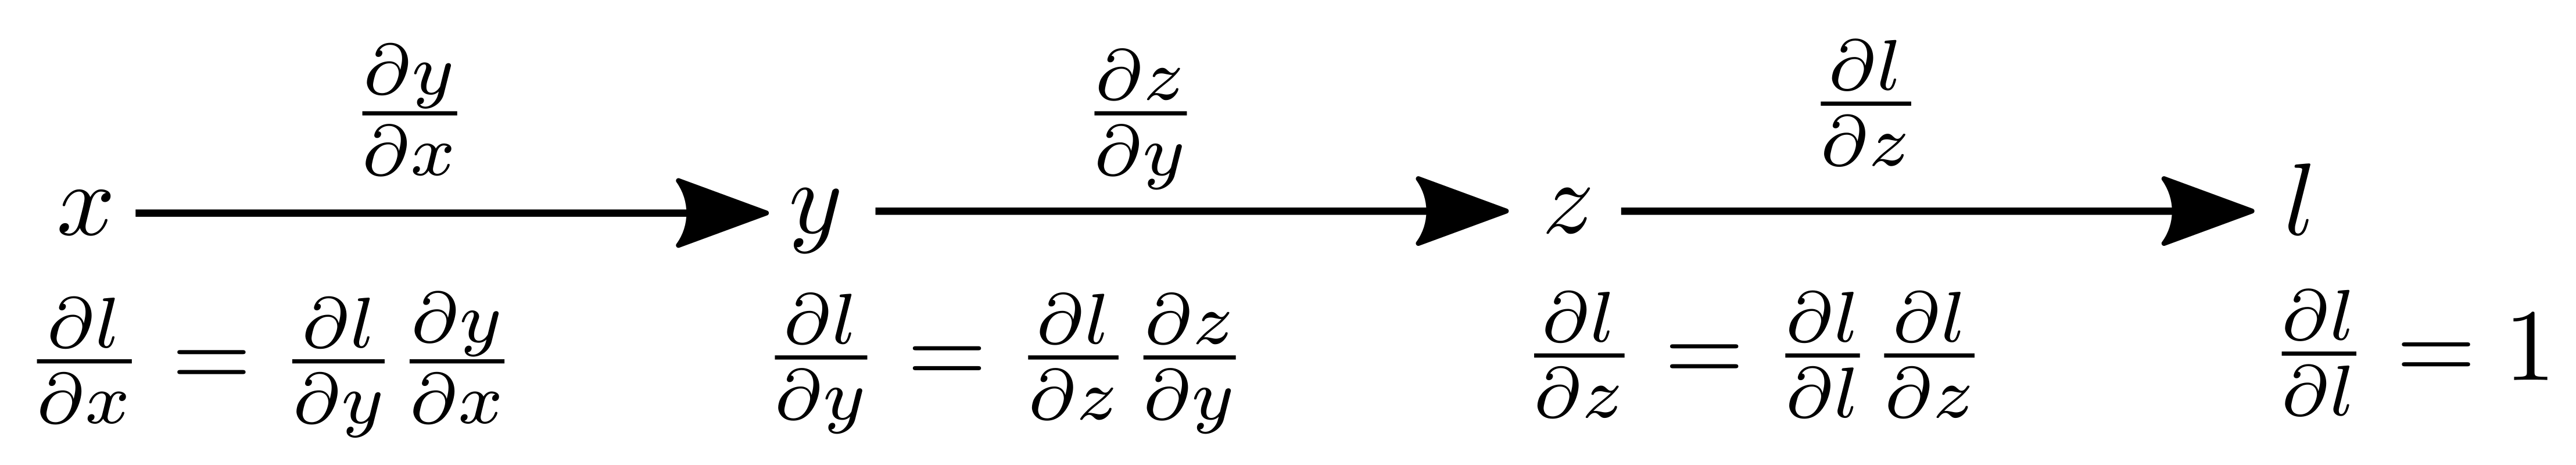
\includegraphics[width=\textwidth]{bp_simple.png}
\end{figure}

\subsection{Backpropagation Through a Neuron}

\begin{figure}[h]
    \centering
    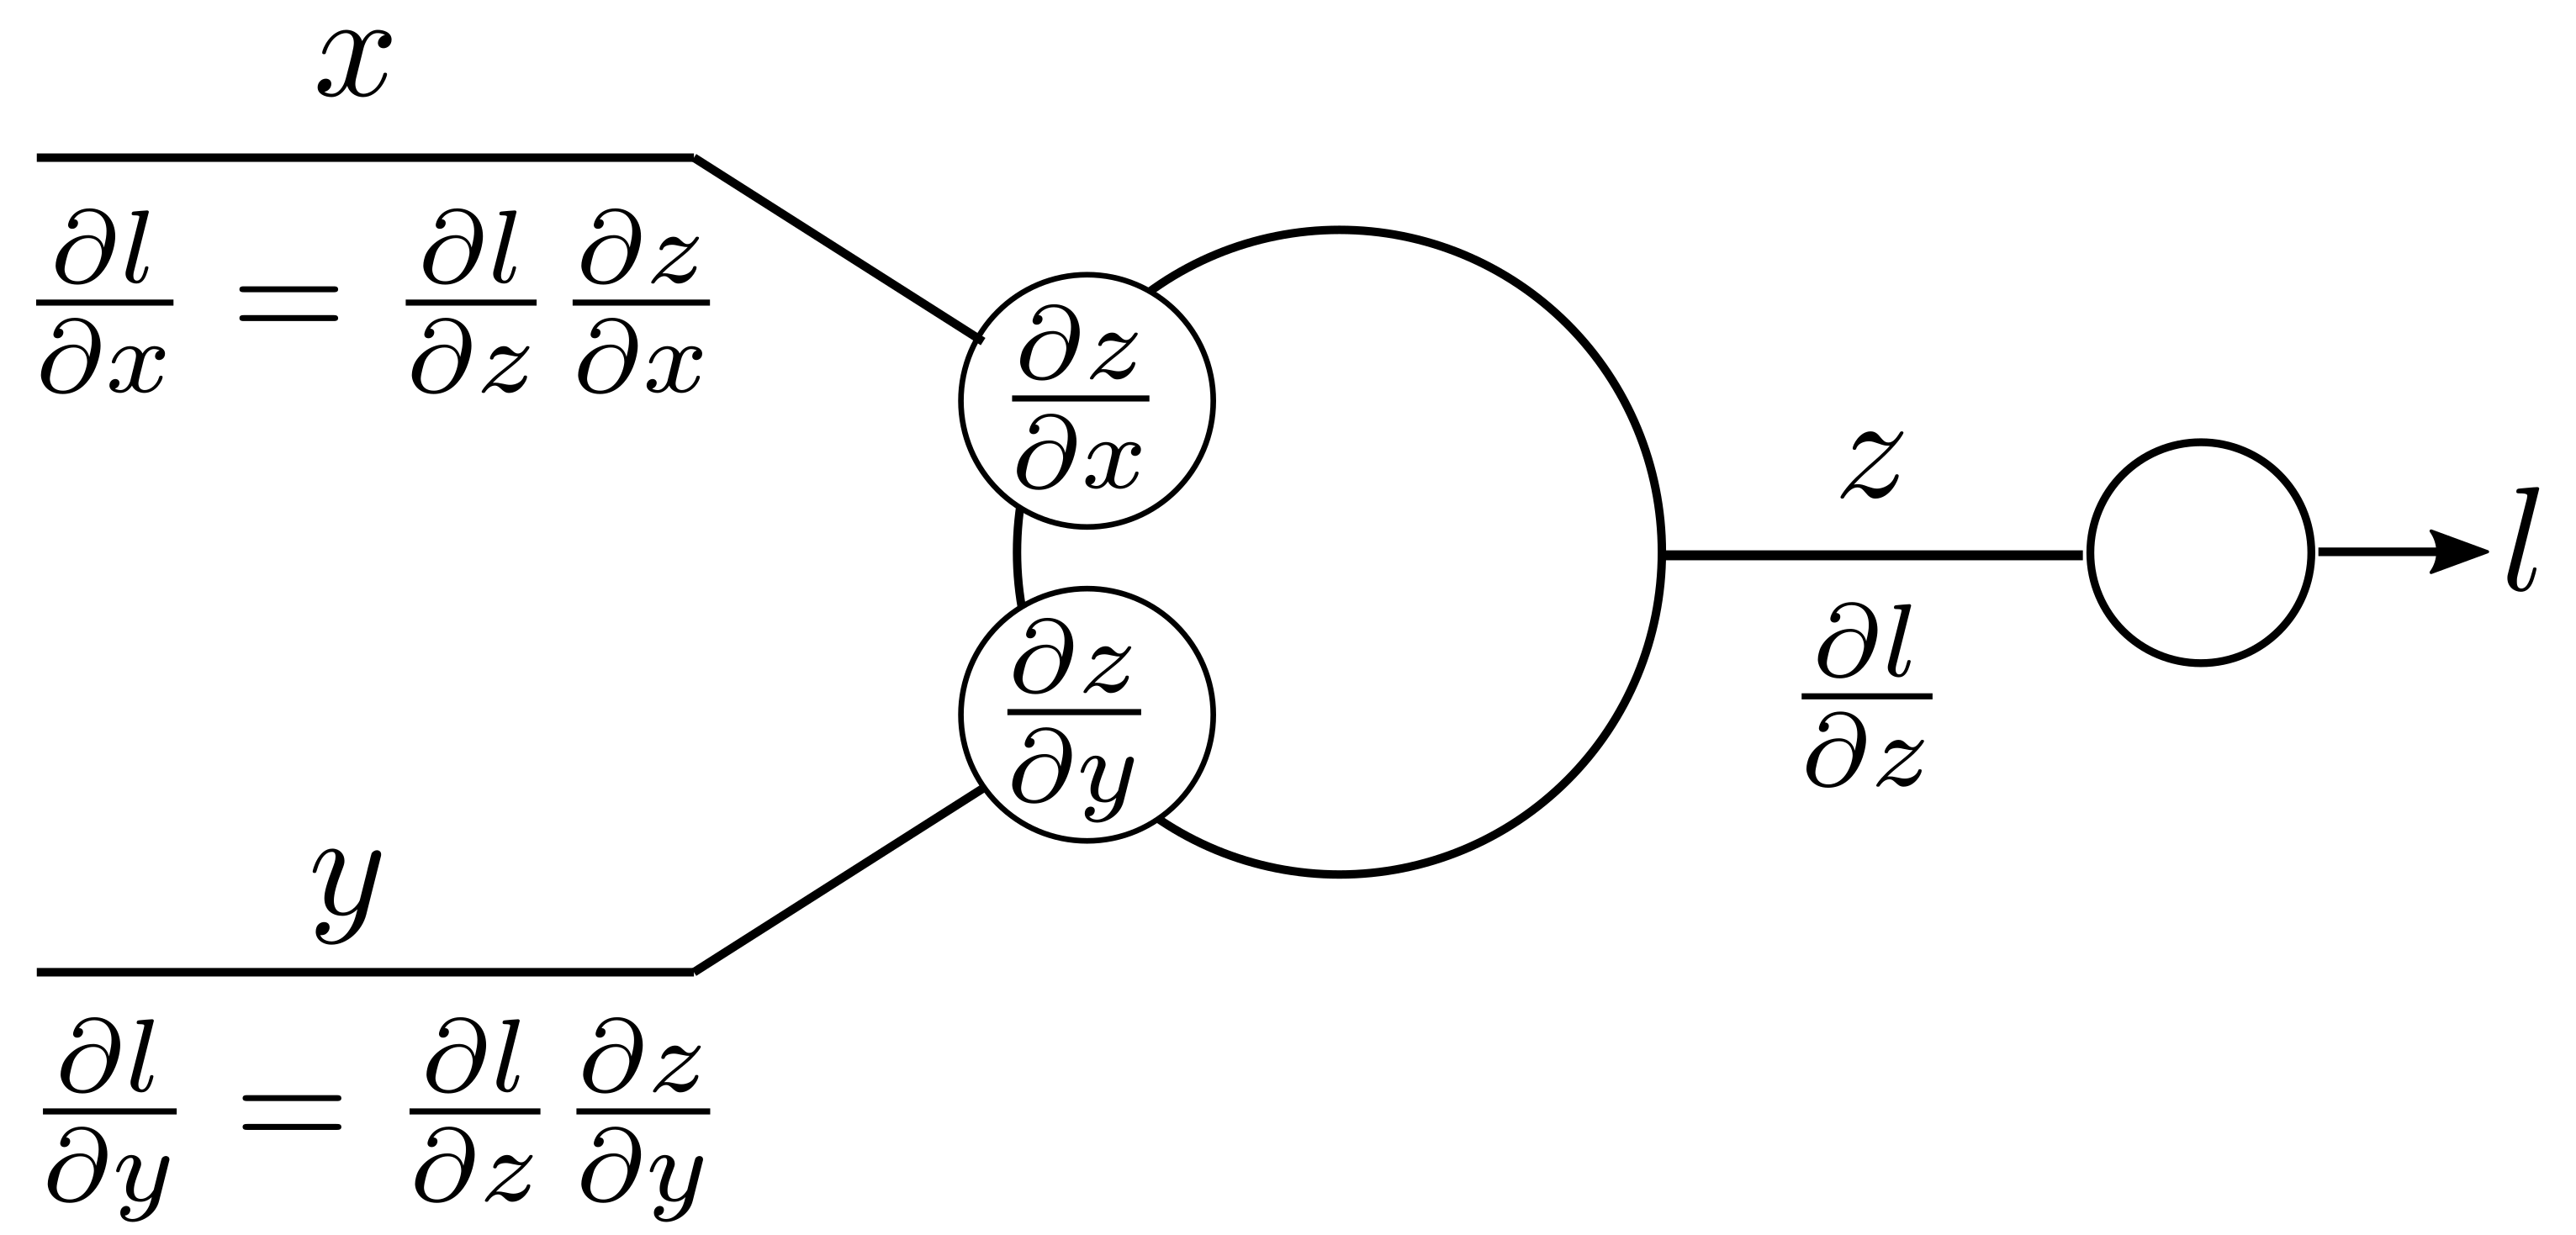
\includegraphics[width=\textwidth]{bp_2_1_neuron.png}
\end{figure}

\subsection{Exercise 1}

\begin{figure}[h]
    \centering
    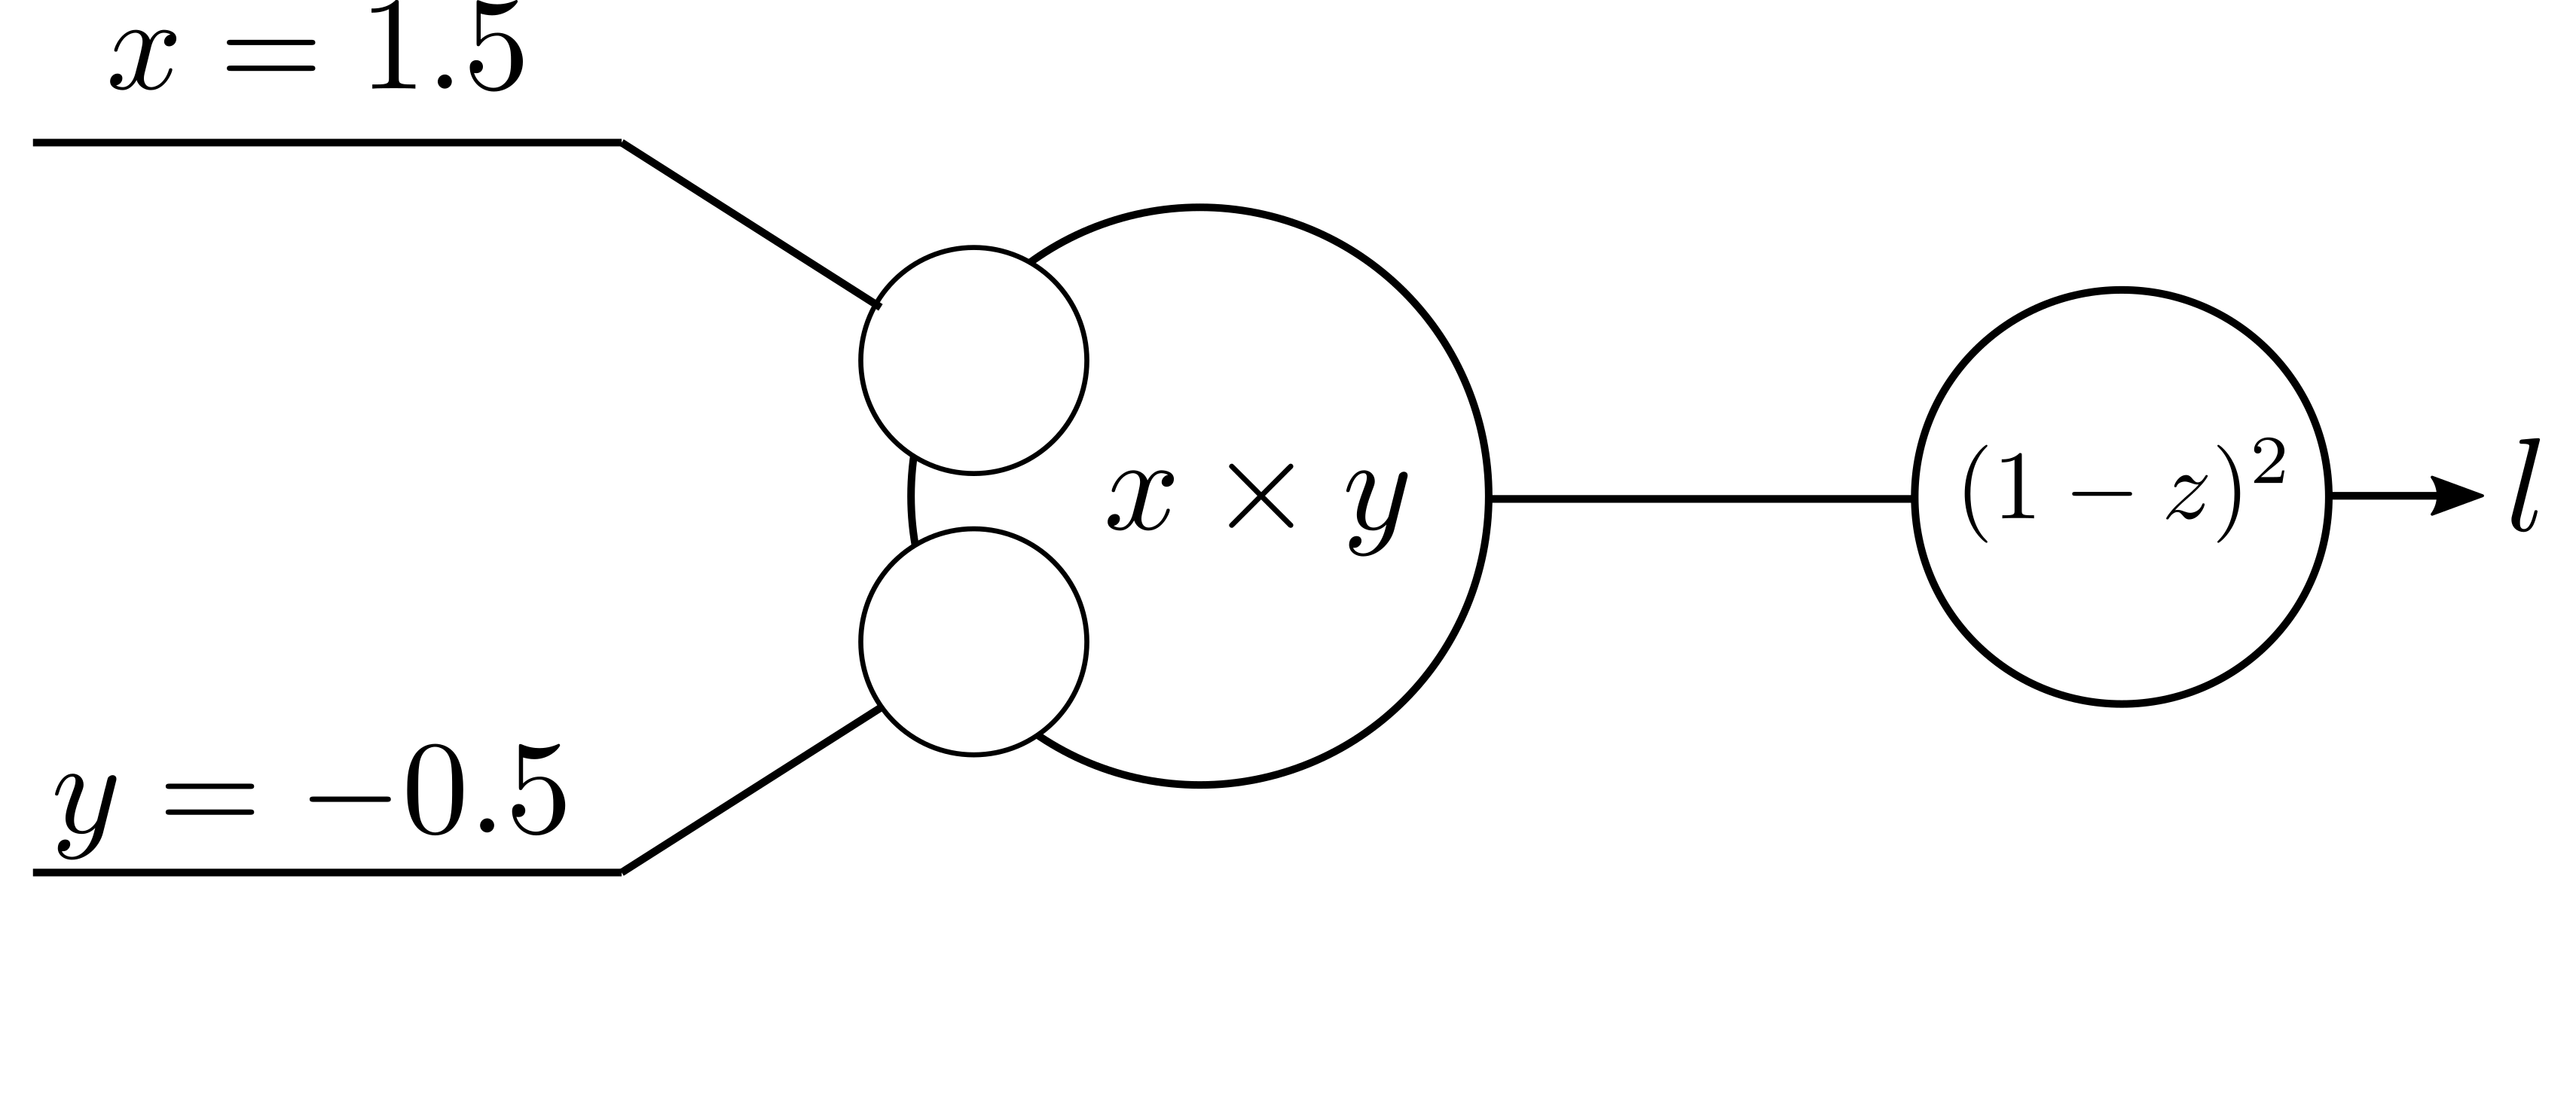
\includegraphics[width=\textwidth]{bp_2_1_neuron_exo.png}
\end{figure}

$\frac{\partial l}{\partial x}$ is equal to:

\begin{itemize}
\item[A/] $1.75$
\item[B/] $-2.25$
\item[C/] $-1.5$
\item[D/] $0.75$
\end{itemize}

\subsection{Exercise 1: Solution}

\begin{figure}[h]
    \centering
    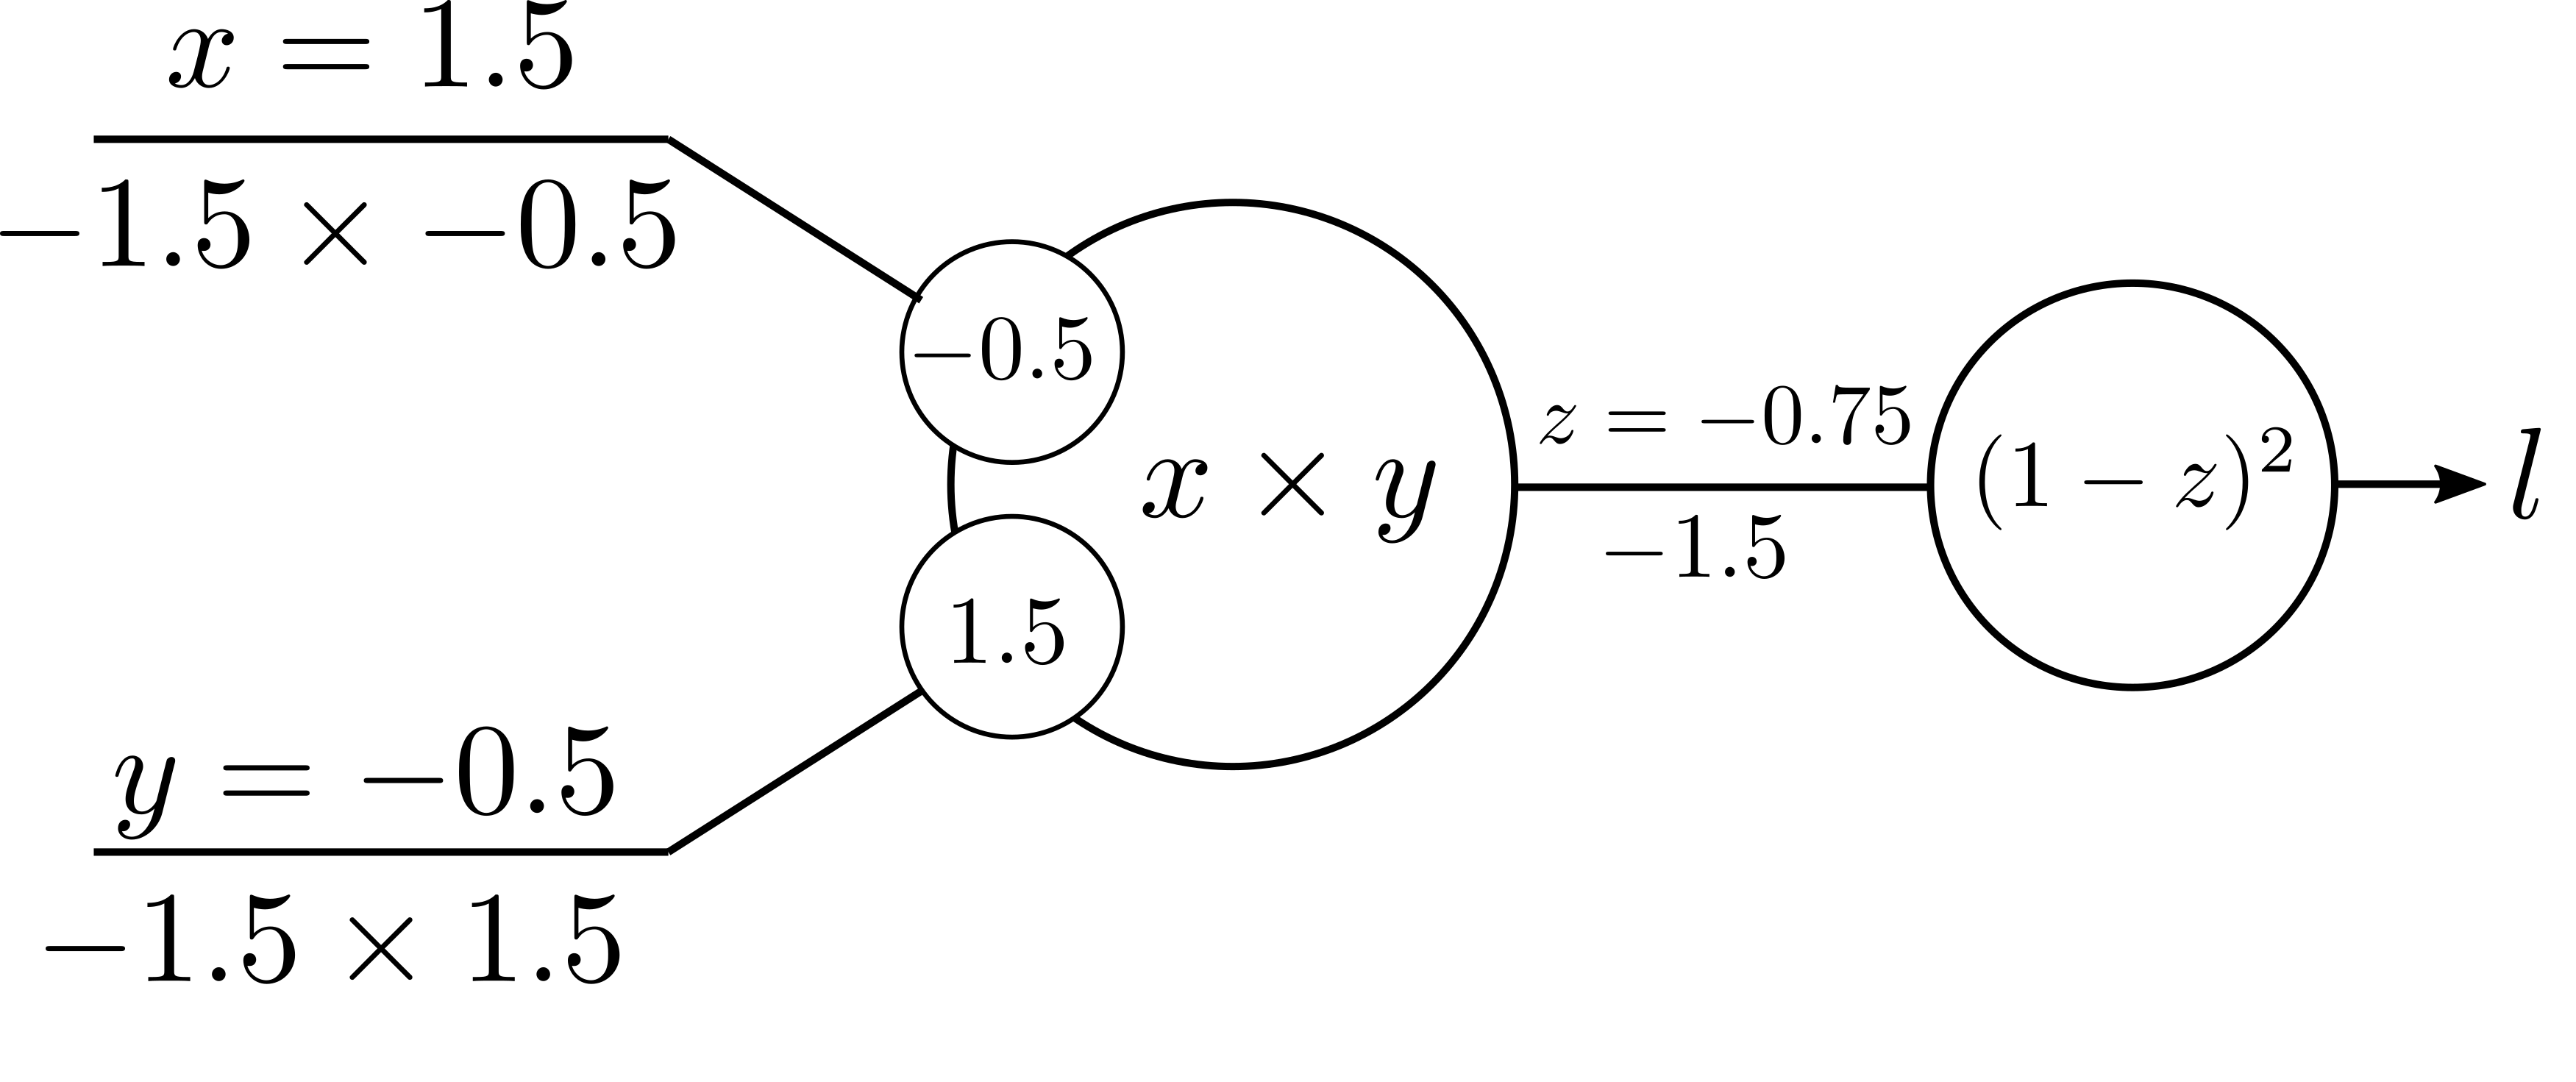
\includegraphics[width=\textwidth]{bp_2_1_neuron_exo_sol.png}
\end{figure}

\subsection{Exercise 2}

\begin{figure}[h]
    \centering
    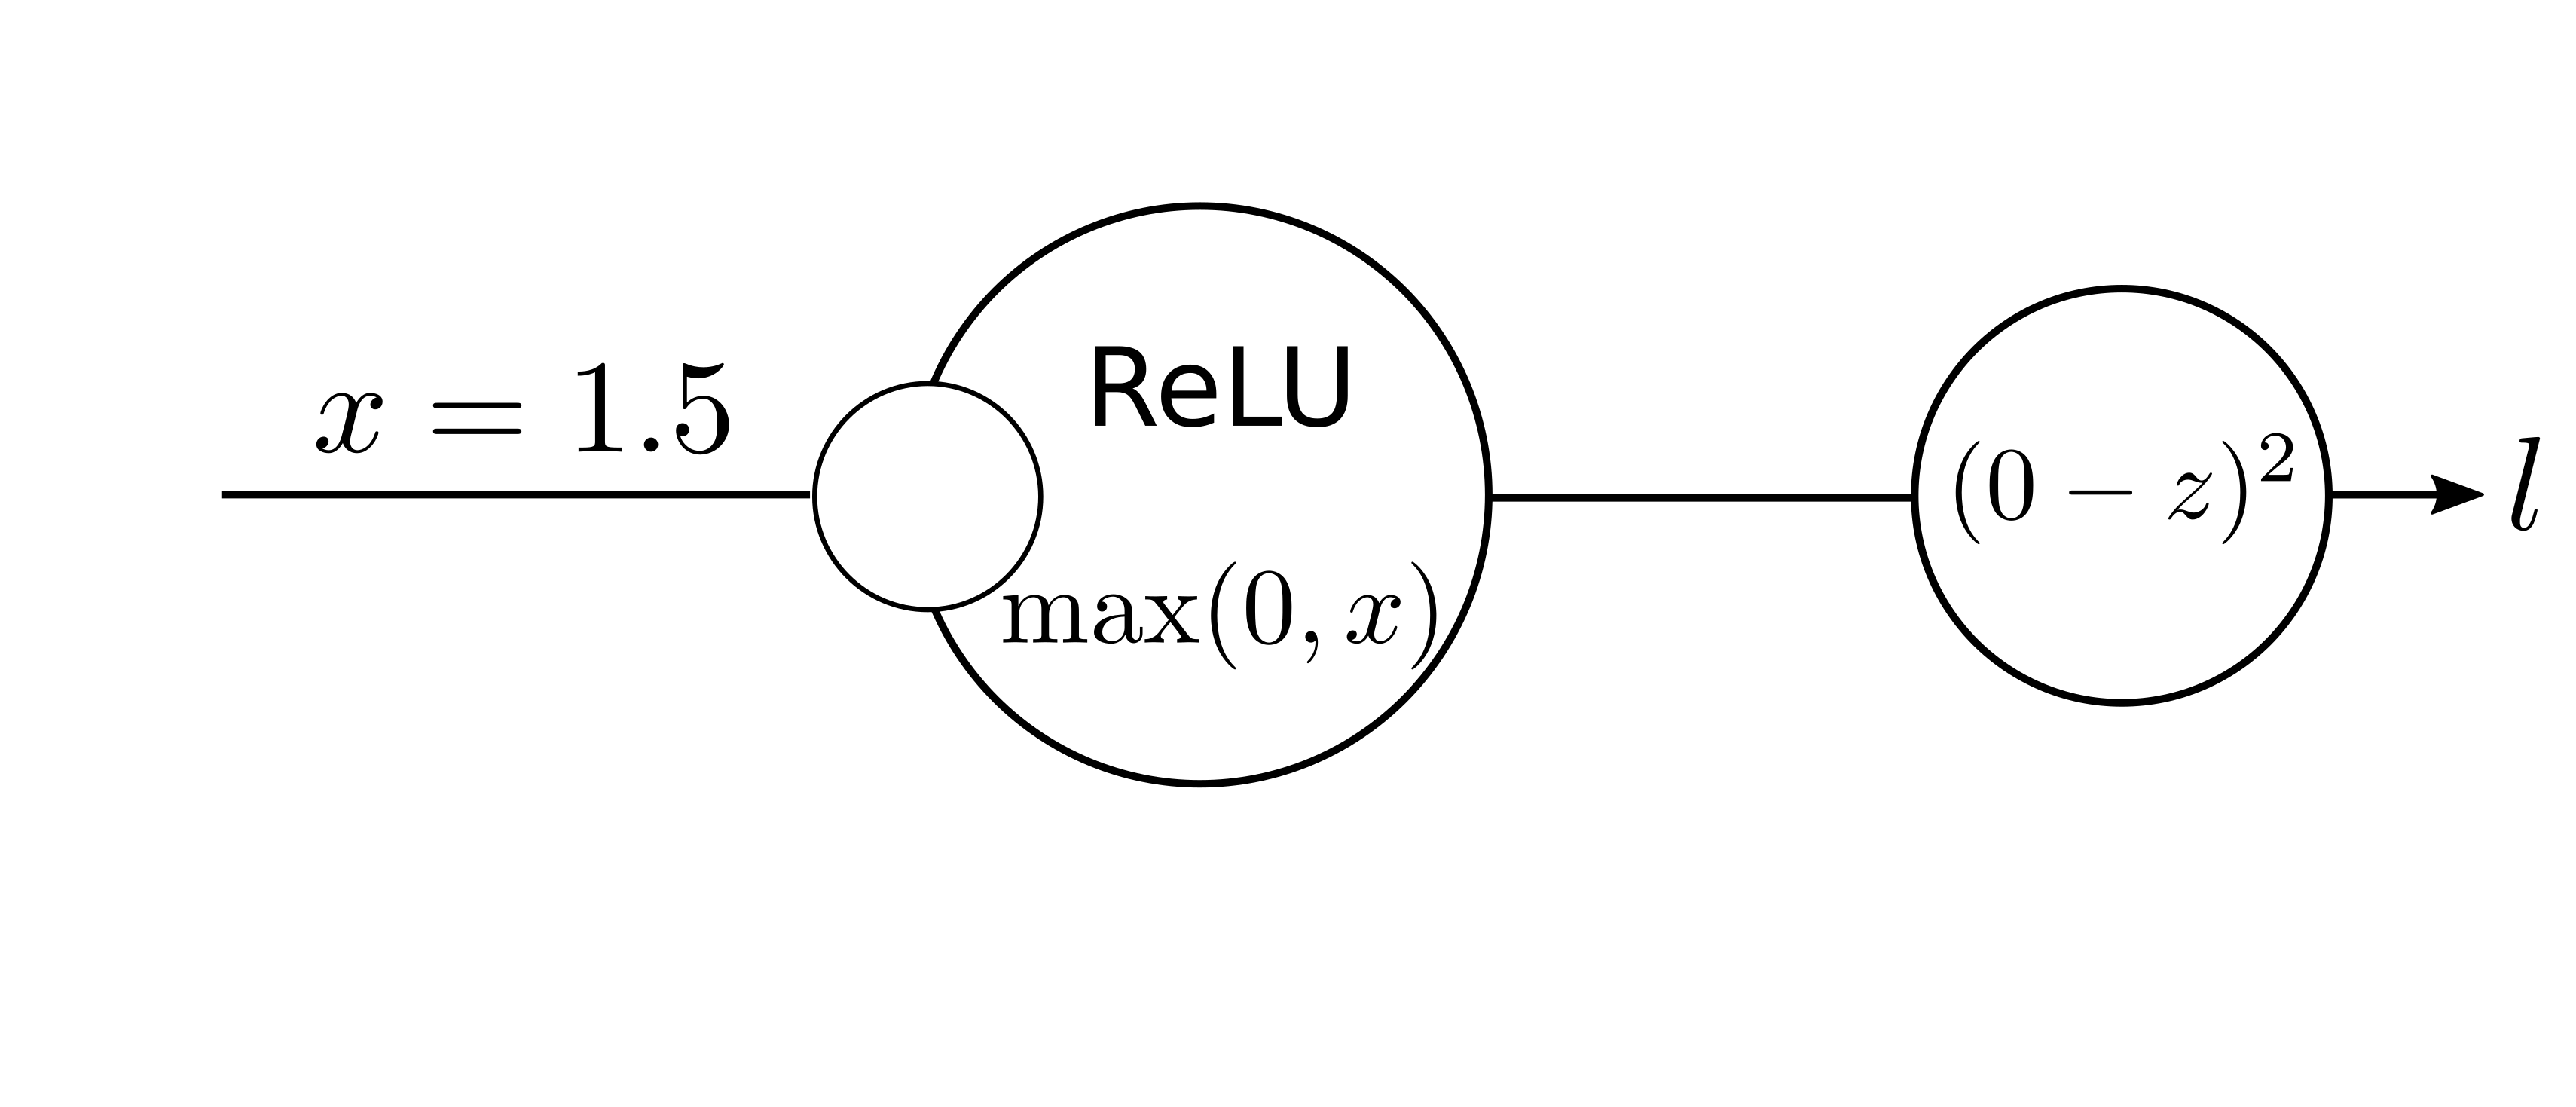
\includegraphics[width=\textwidth]{bp_relu_exo.png}
\end{figure}

\subsection{Exercise 2: Solution}

\begin{figure}[h]
    \centering
    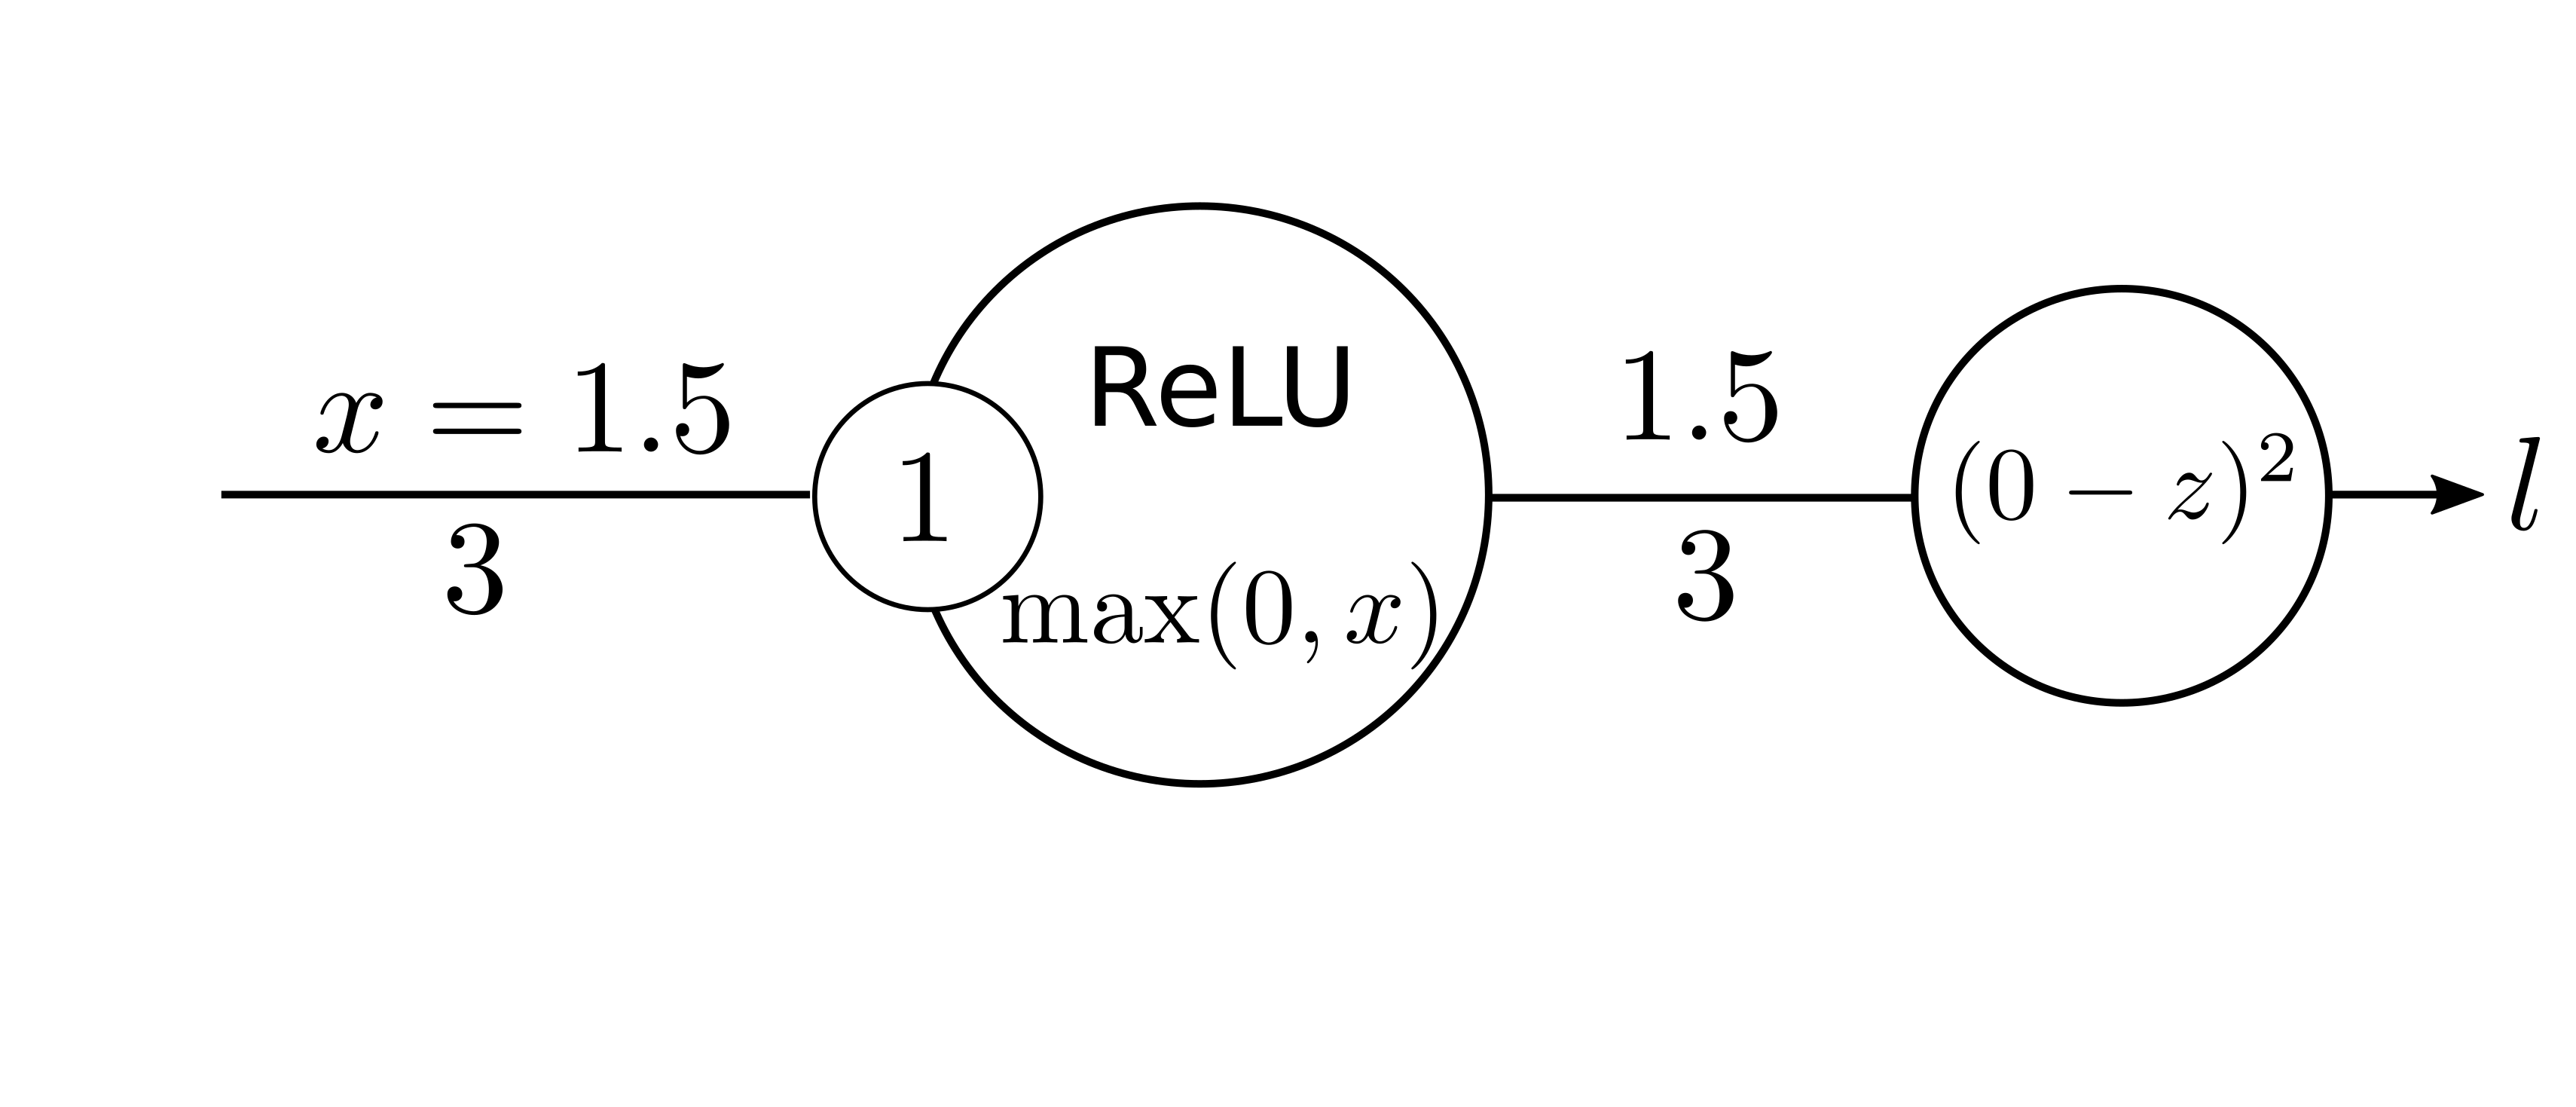
\includegraphics[width=\textwidth]{bp_relu_exo_sol.png}
\end{figure}

\subsection{Exercise 3}

\begin{figure}[h]
    \centering
    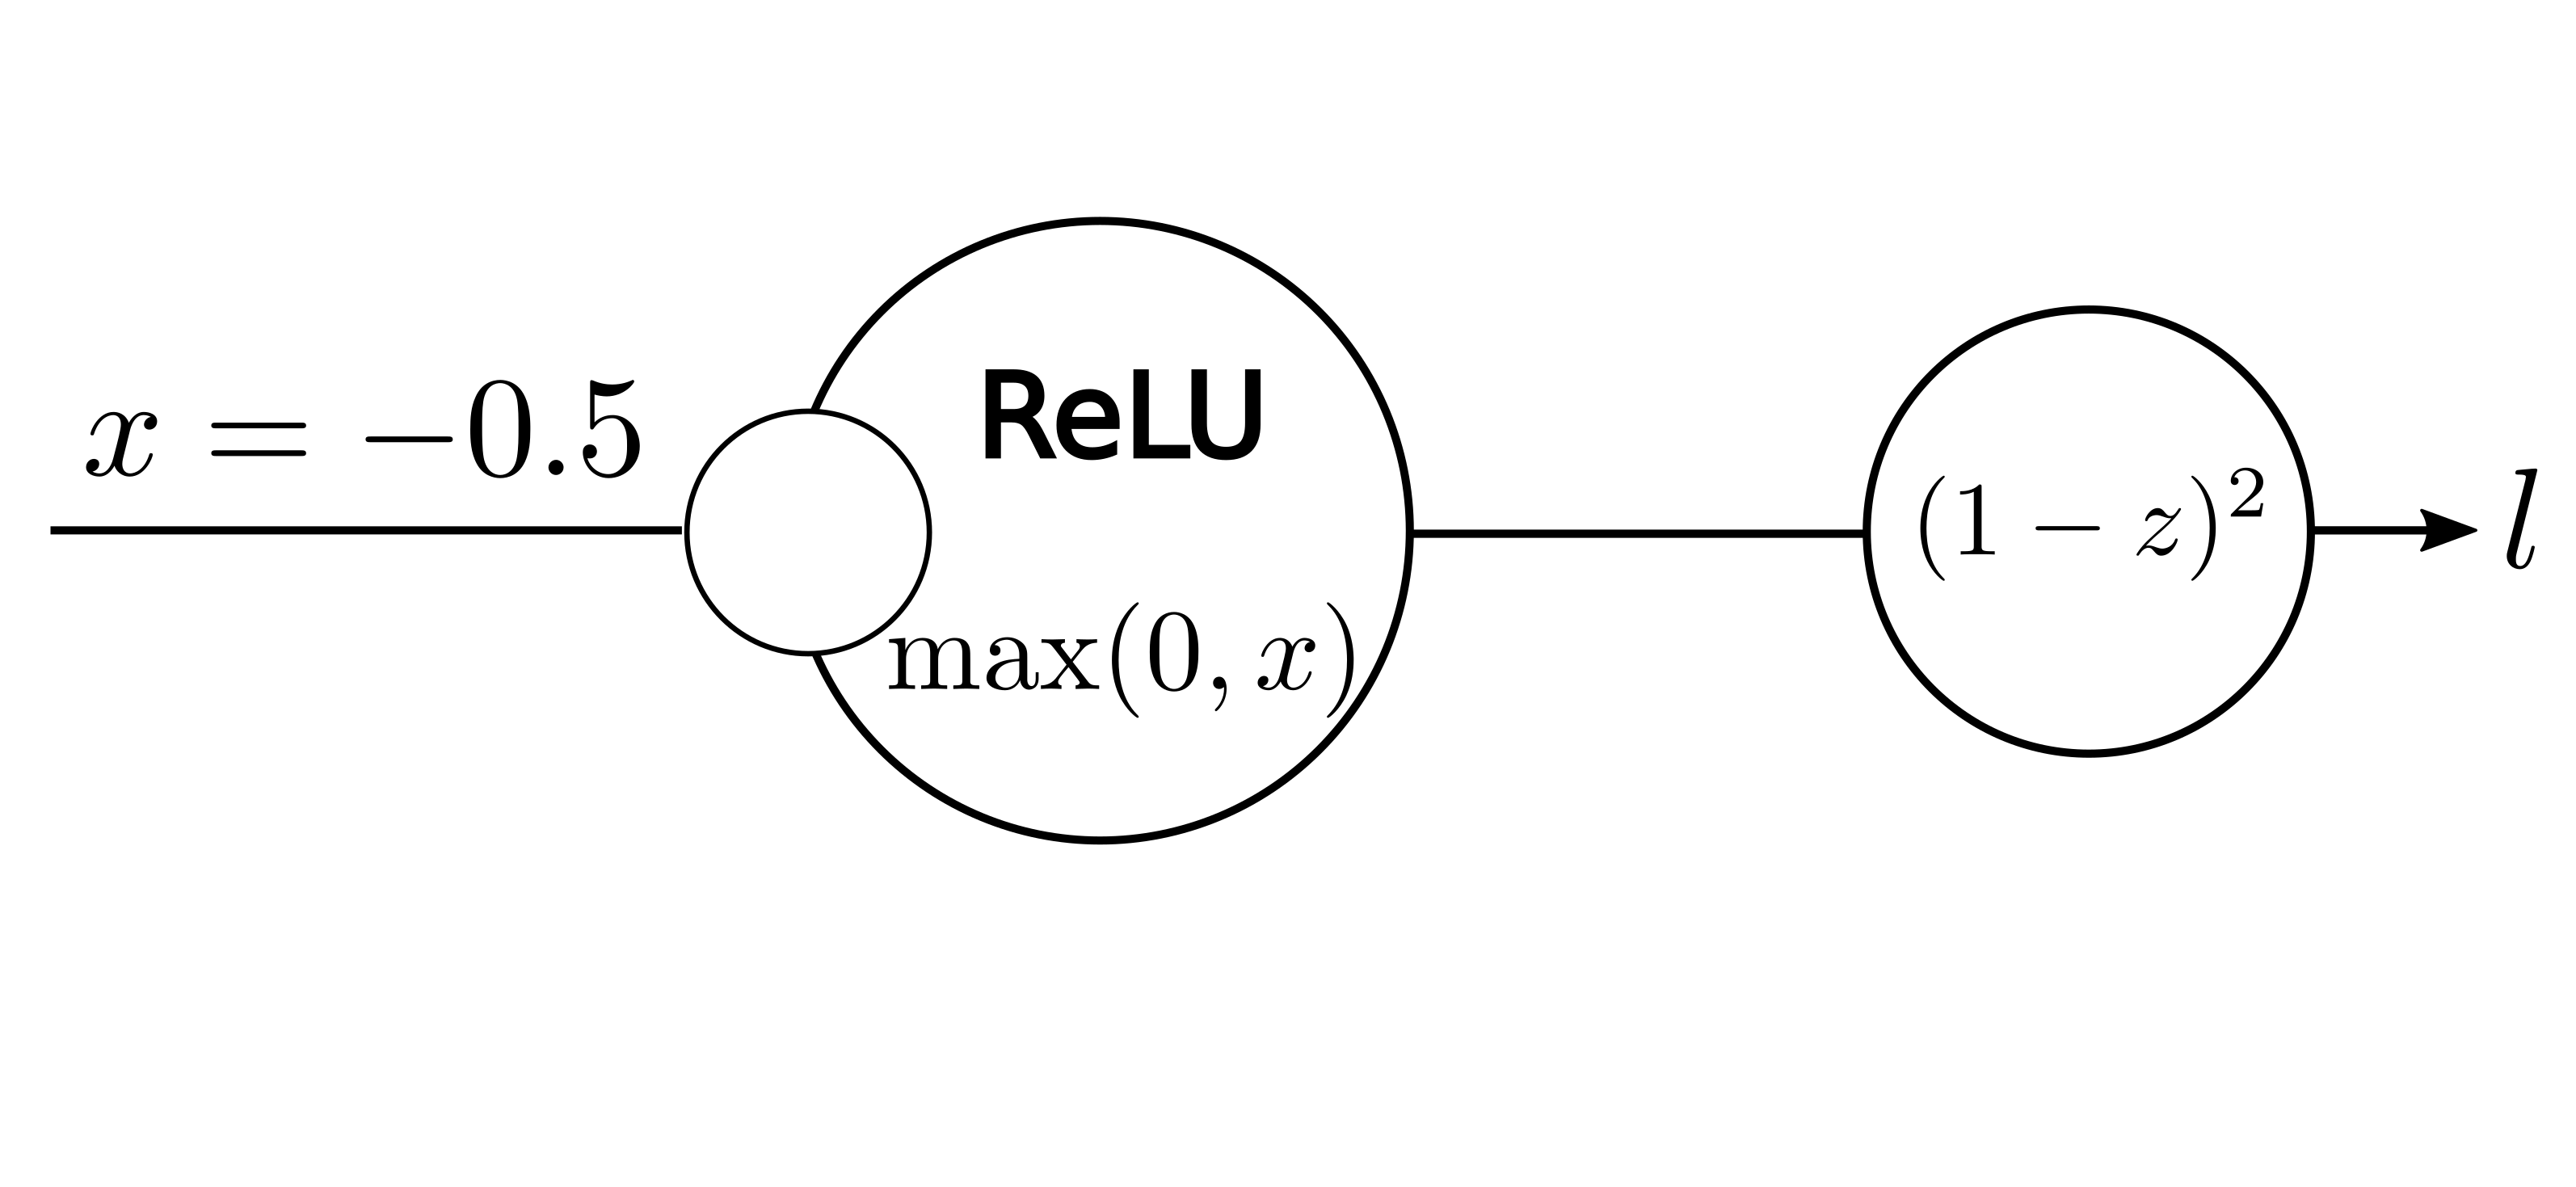
\includegraphics[width=\textwidth]{bp_relu_exo2.png}
\end{figure}

\subsection{Exercise 3: Solution}

\begin{figure}[h]
    \centering
    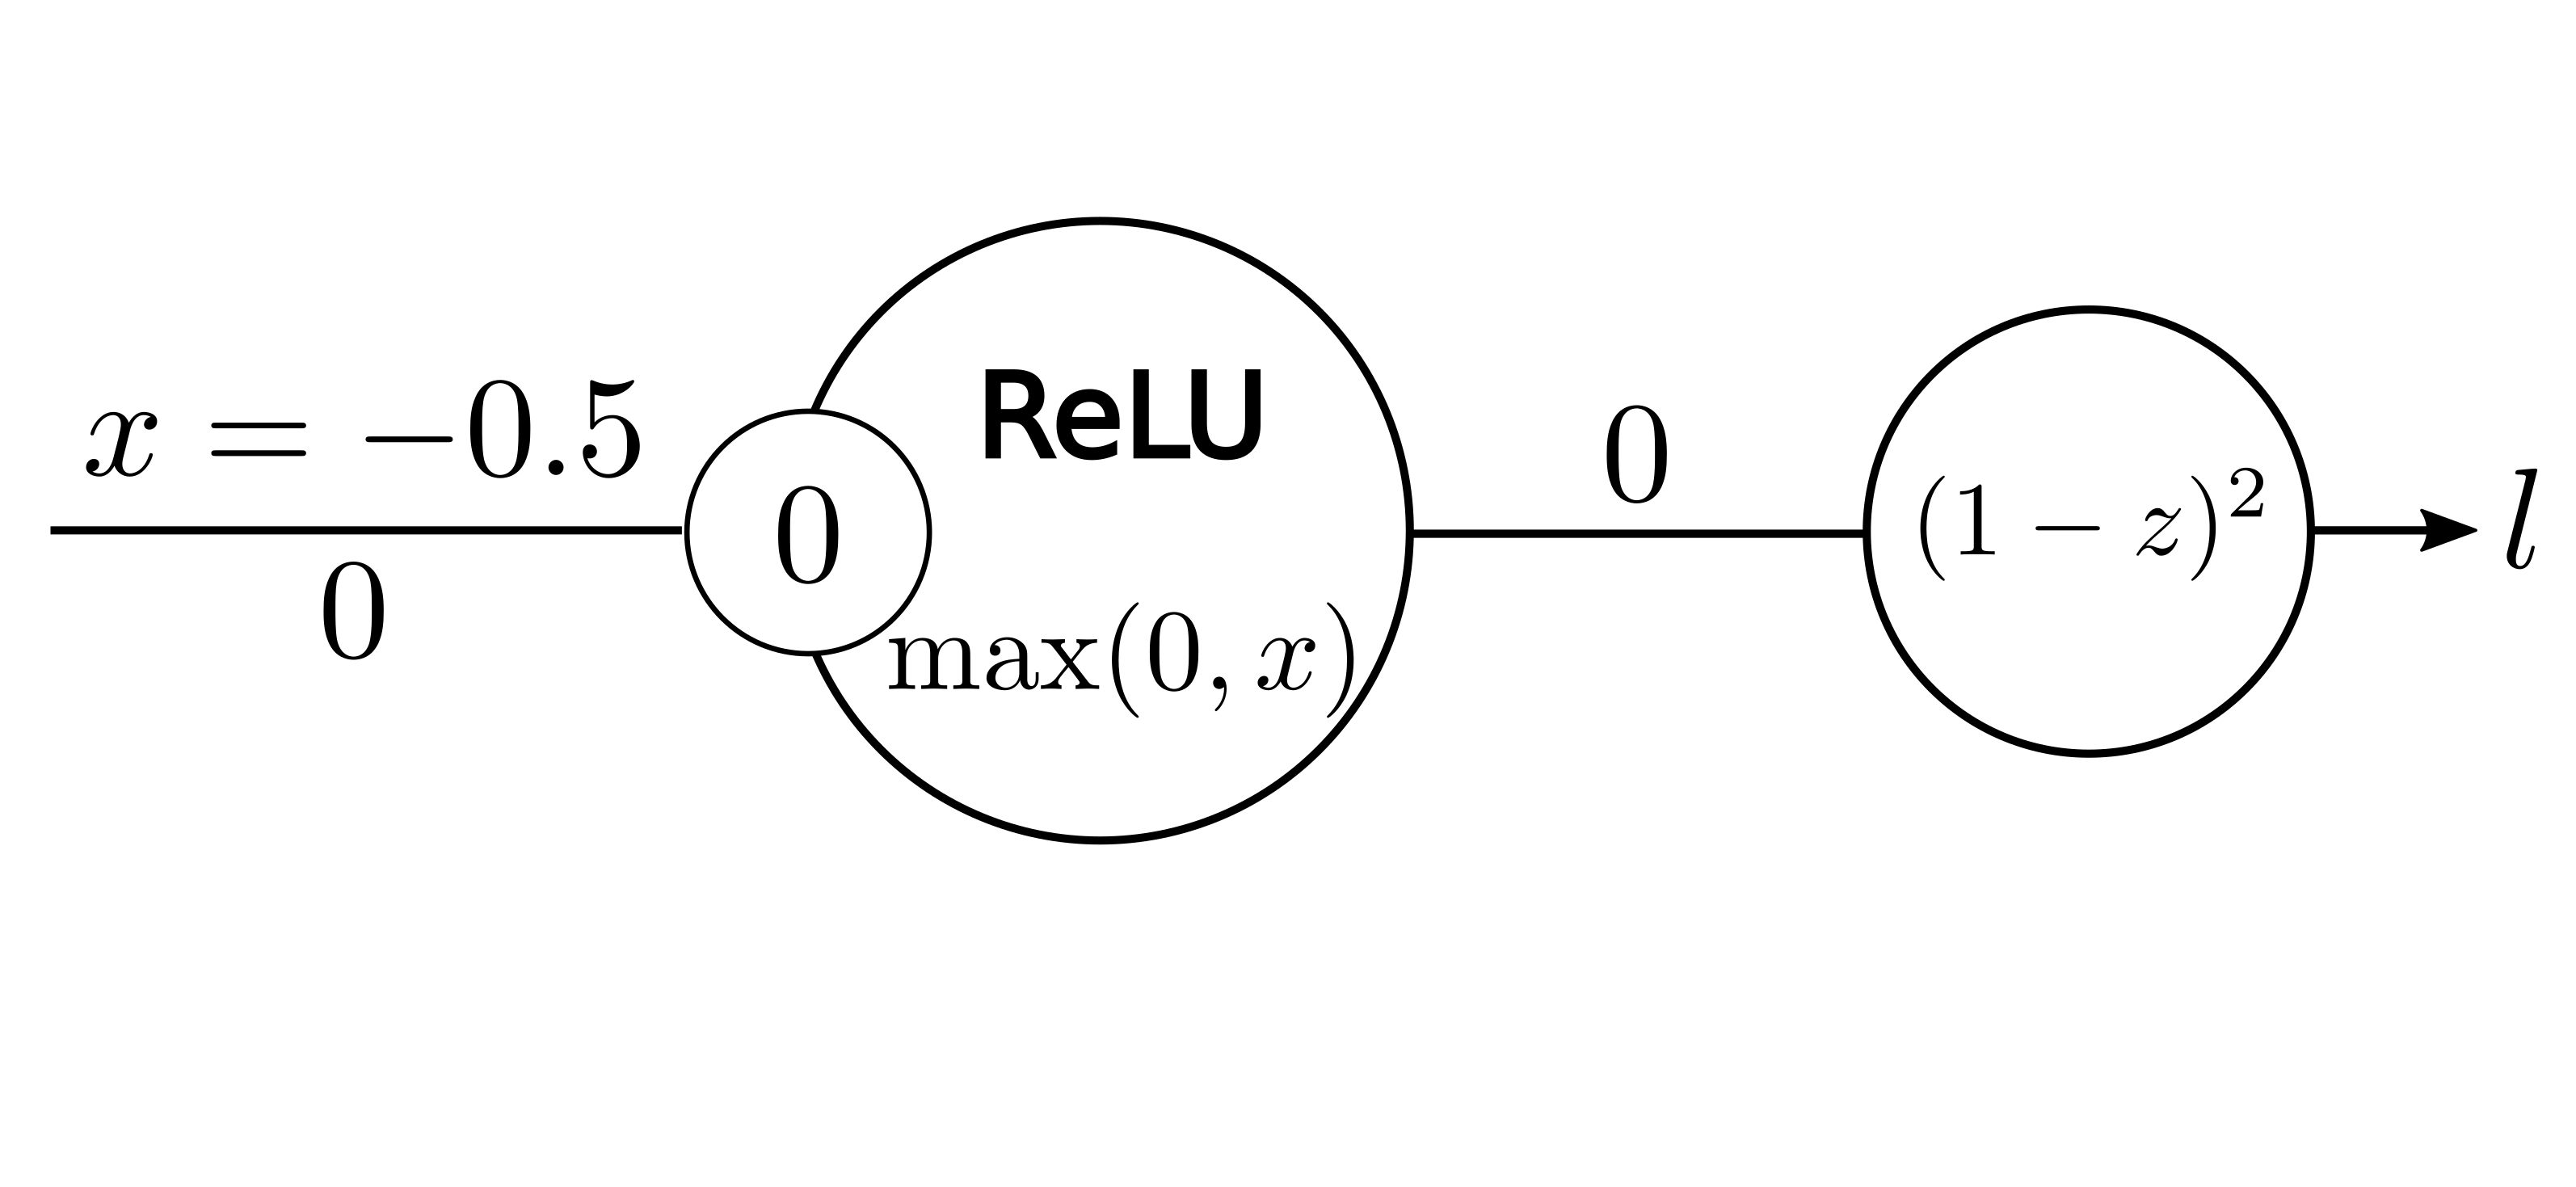
\includegraphics[width=\textwidth]{bp_relu_exo2_sol.png}
\end{figure}

\subsection{Exercise 4}

\begin{figure}[h]
    \centering
    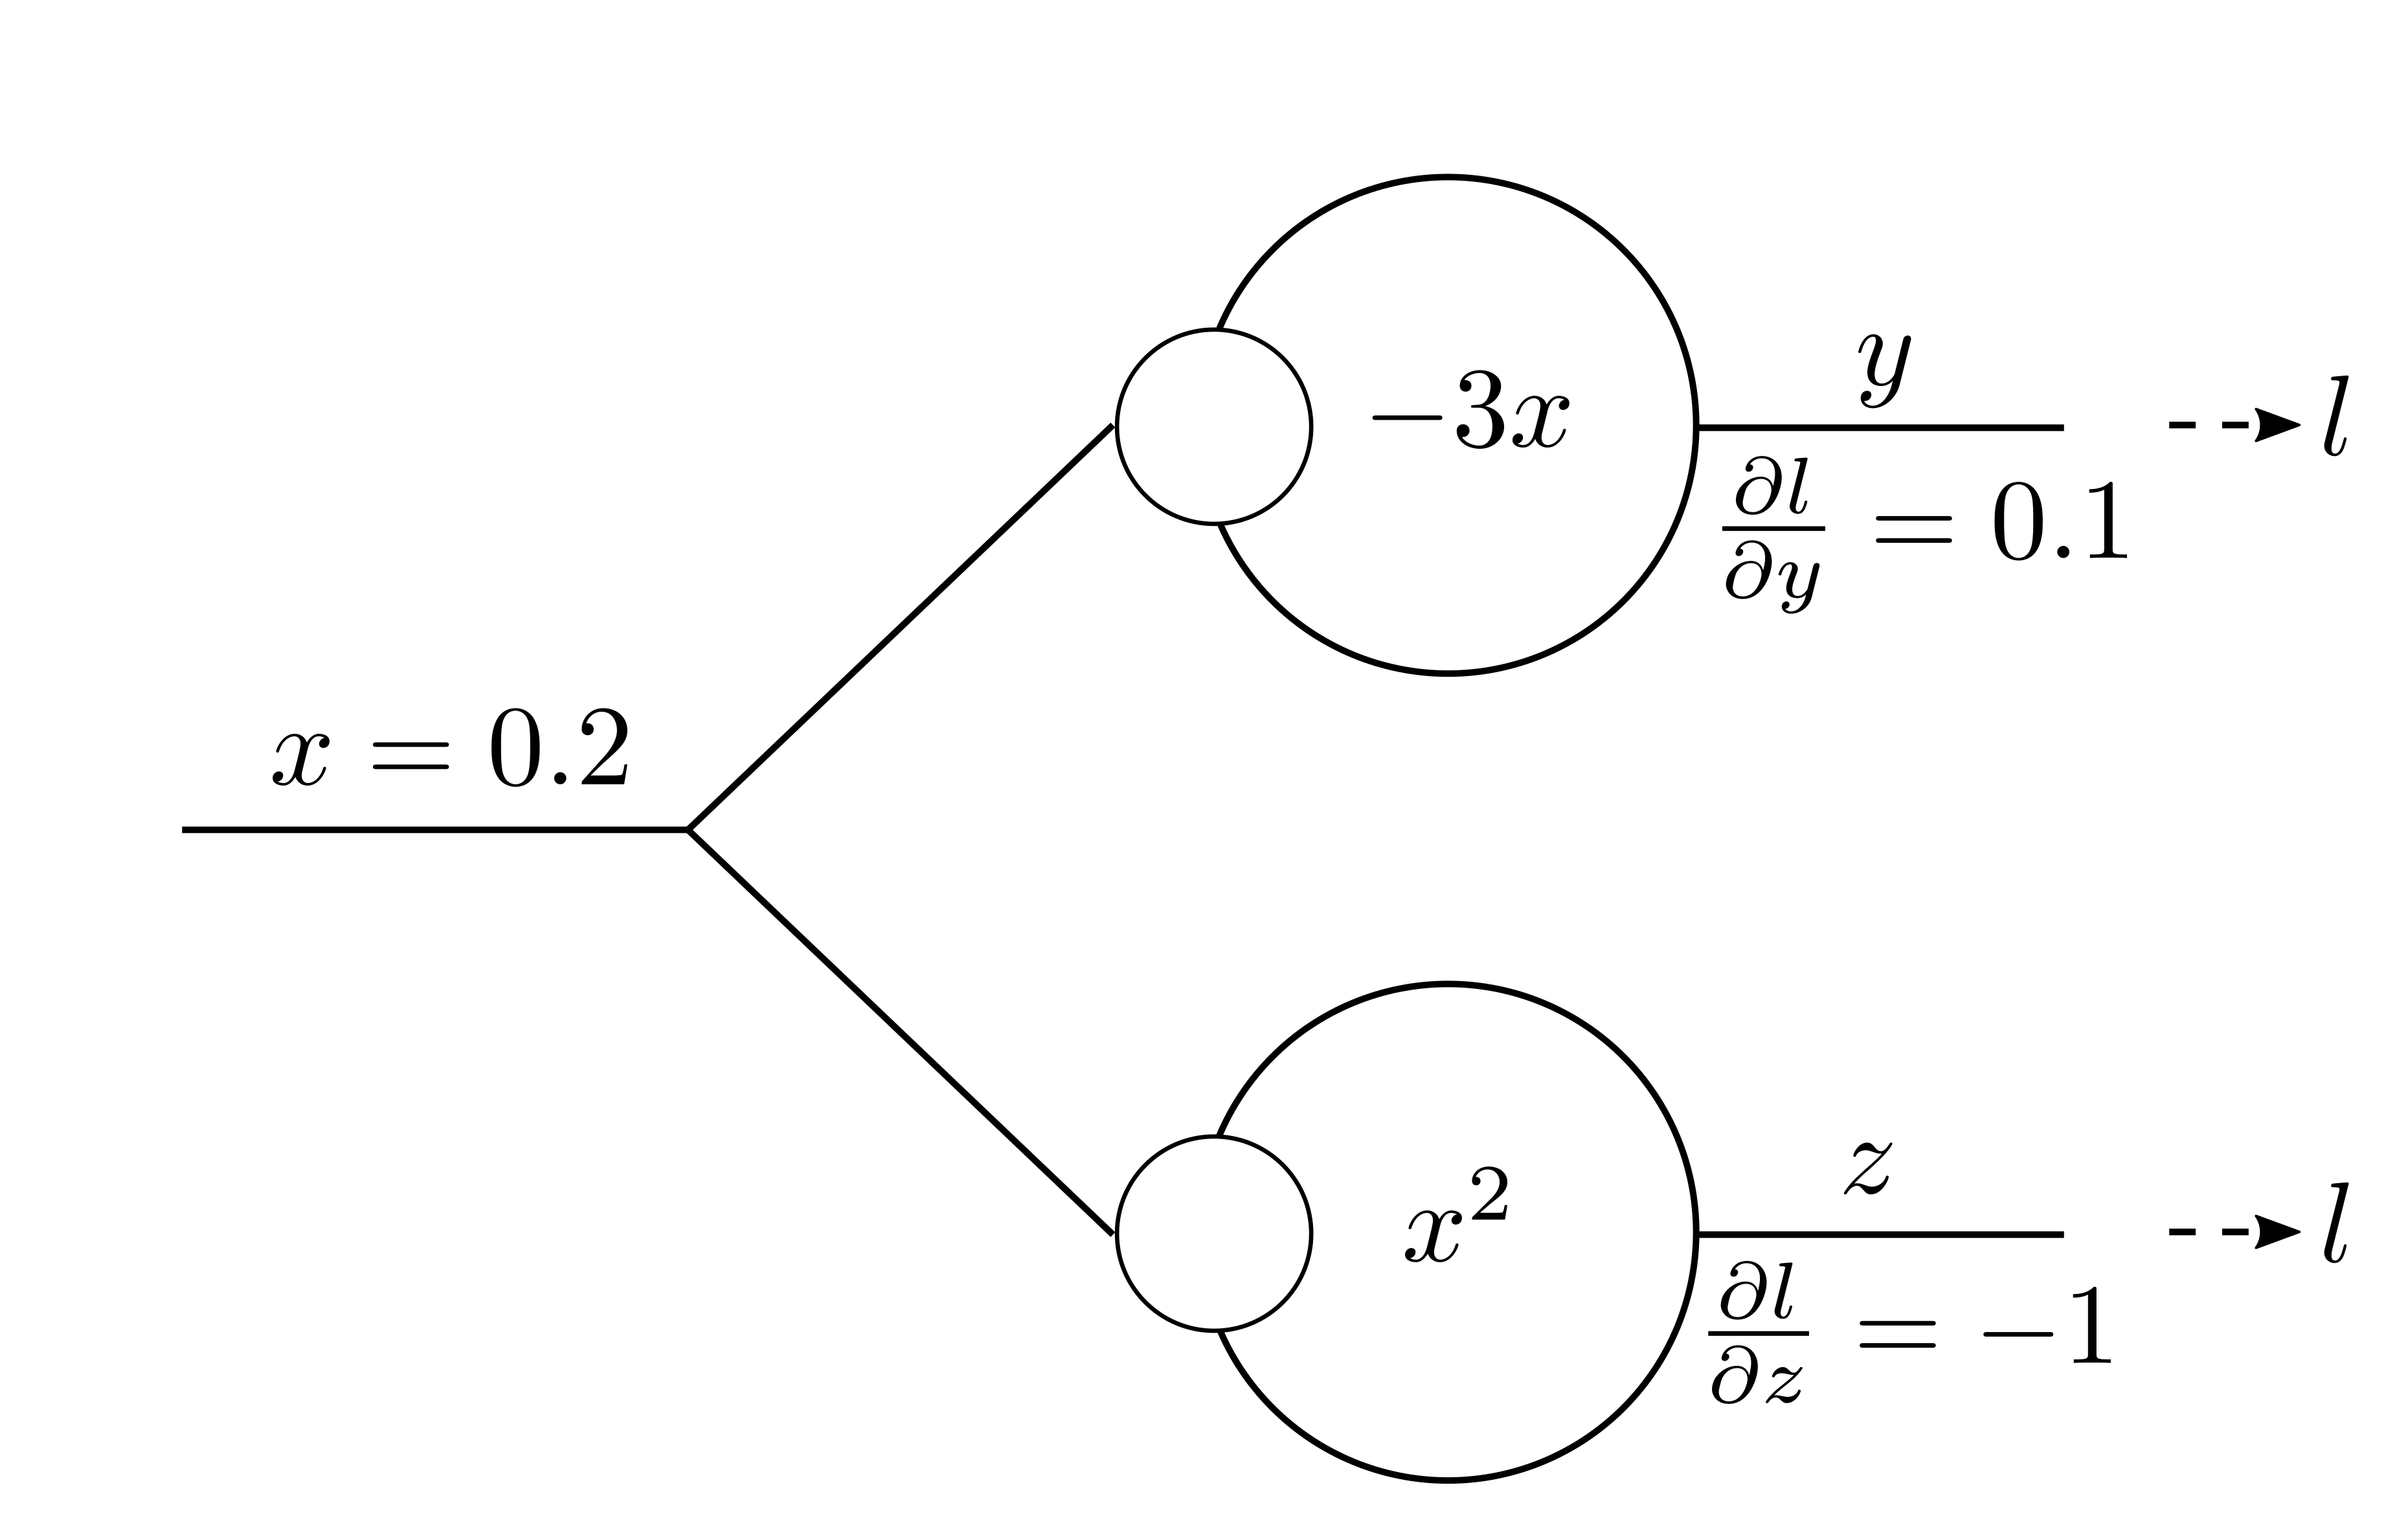
\includegraphics[width=0.8\textwidth]{bp_split.png}
\end{figure}

\begin{block}{Quiz}
What's the value of $\frac{\partial l}{\partial x}$?
\end{block}

\subsection{Exercise 4: Solution}

\begin{figure}[h]
    \centering
    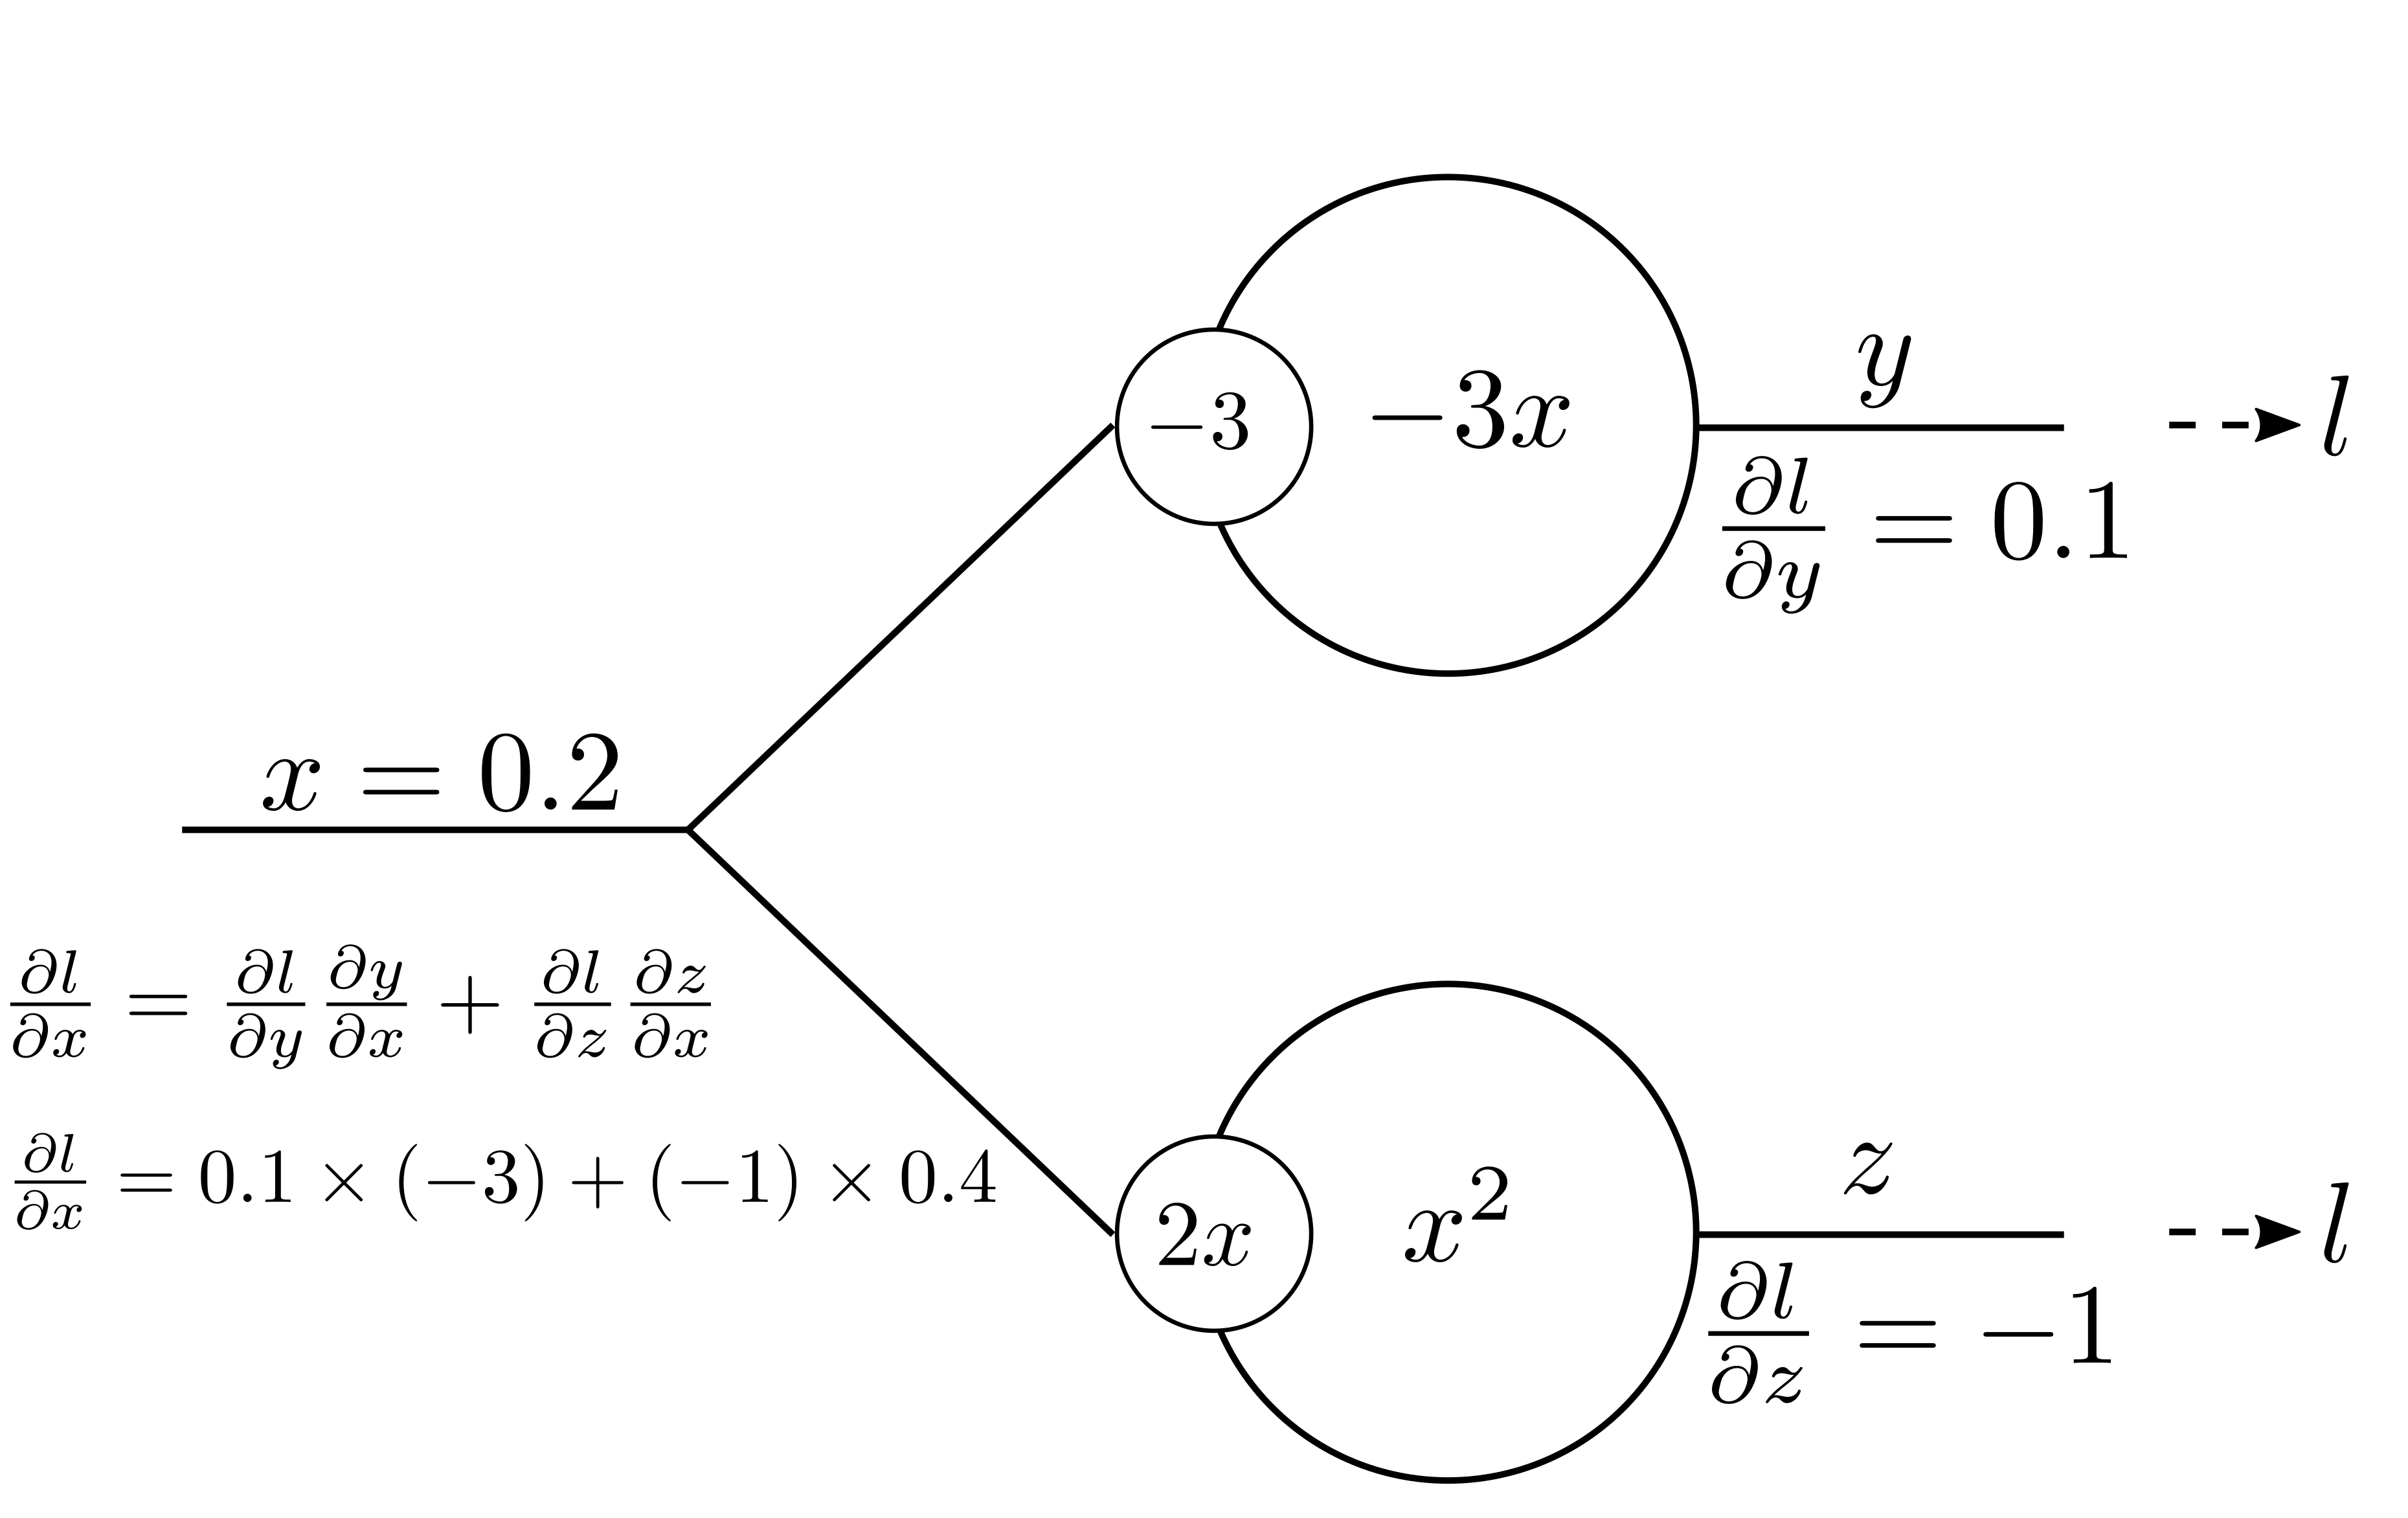
\includegraphics[width=\textwidth]{bp_split_sol.png}
\end{figure}

\subsection{Vector Calculus}

\begin{itemize}
\item $L$ and $V$ are differentiable functions.
\end{itemize}

\begin{figure}[h]
    \centering
    \begin{subfigure}{.5\textwidth}
        \begin{equation*}
        \begin{split}
        L: \R^n & \longrightarrow \R\\
        \x & \longmapsto L(\x)
        \end{split}
        \end{equation*}
        \begin{block}{Gradient}
        \centering
        $\nabla_\x L = \frac{\partial L}{\partial \x} = (\frac{\partial L}{\partial x_1}, \ldots, \frac{\partial L}{\partial x_n}) $
        \end{block}
    \end{subfigure}
    \begin{subfigure}{.5\textwidth}
        \begin{equation*}
        \begin{split}
        V: \R^p & \longrightarrow \R^q\\
        \y & \longmapsto V(\y)
        \end{split}
        \end{equation*}
        \begin{block}{Jacobian}
        \centering
        $J(V) = \frac{\partial V}{\partial \y} =
        \begin{pmatrix}
        \frac{\partial V_1}{\partial y_1} & \cdots & \frac{\partial V_1}{\partial y_p} \\
        \vdots & \ddots & \vdots \\
        \frac{\partial V_q}{\partial y_1} & \cdots & \frac{\partial V_q}{\partial y_p}
        \end{pmatrix}
        $
        \end{block}
    \end{subfigure}
\end{figure}

\subsection{Matrix Calculus}

\begin{itemize}
\item Function $\mathcal{M}$ is differentiable.
\end{itemize}

\begin{equation*}
\begin{split}
\mathcal{M}: \R^{(m,n)} & \longrightarrow \R^{(p,q)}\\
\X & \longmapsto \mathcal{M}(M)
\end{split}
\end{equation*}

\begin{block}{}
\centering
$\frac{\partial \mathcal{M}}{\partial \X} =
\begin{pmatrix}
\frac{\partial \mathcal{M}_{1,1}}{\partial \X} & \cdots & \frac{\partial \mathcal{M}_{1,q}}{\partial \X} \\
\vdots & \ddots & \vdots \\
\frac{\partial \mathcal{M}_{p,q}}{\partial \X} & \cdots & \frac{\partial \mathcal{M}_{p,q}}{\partial \X}
\end{pmatrix}
$

\end{block}

This is an array of size $(m, n, p, q)$.

\subsection{Backpropagation Through an Activation Function $g$}

\begin{figure}[h]
    \centering
    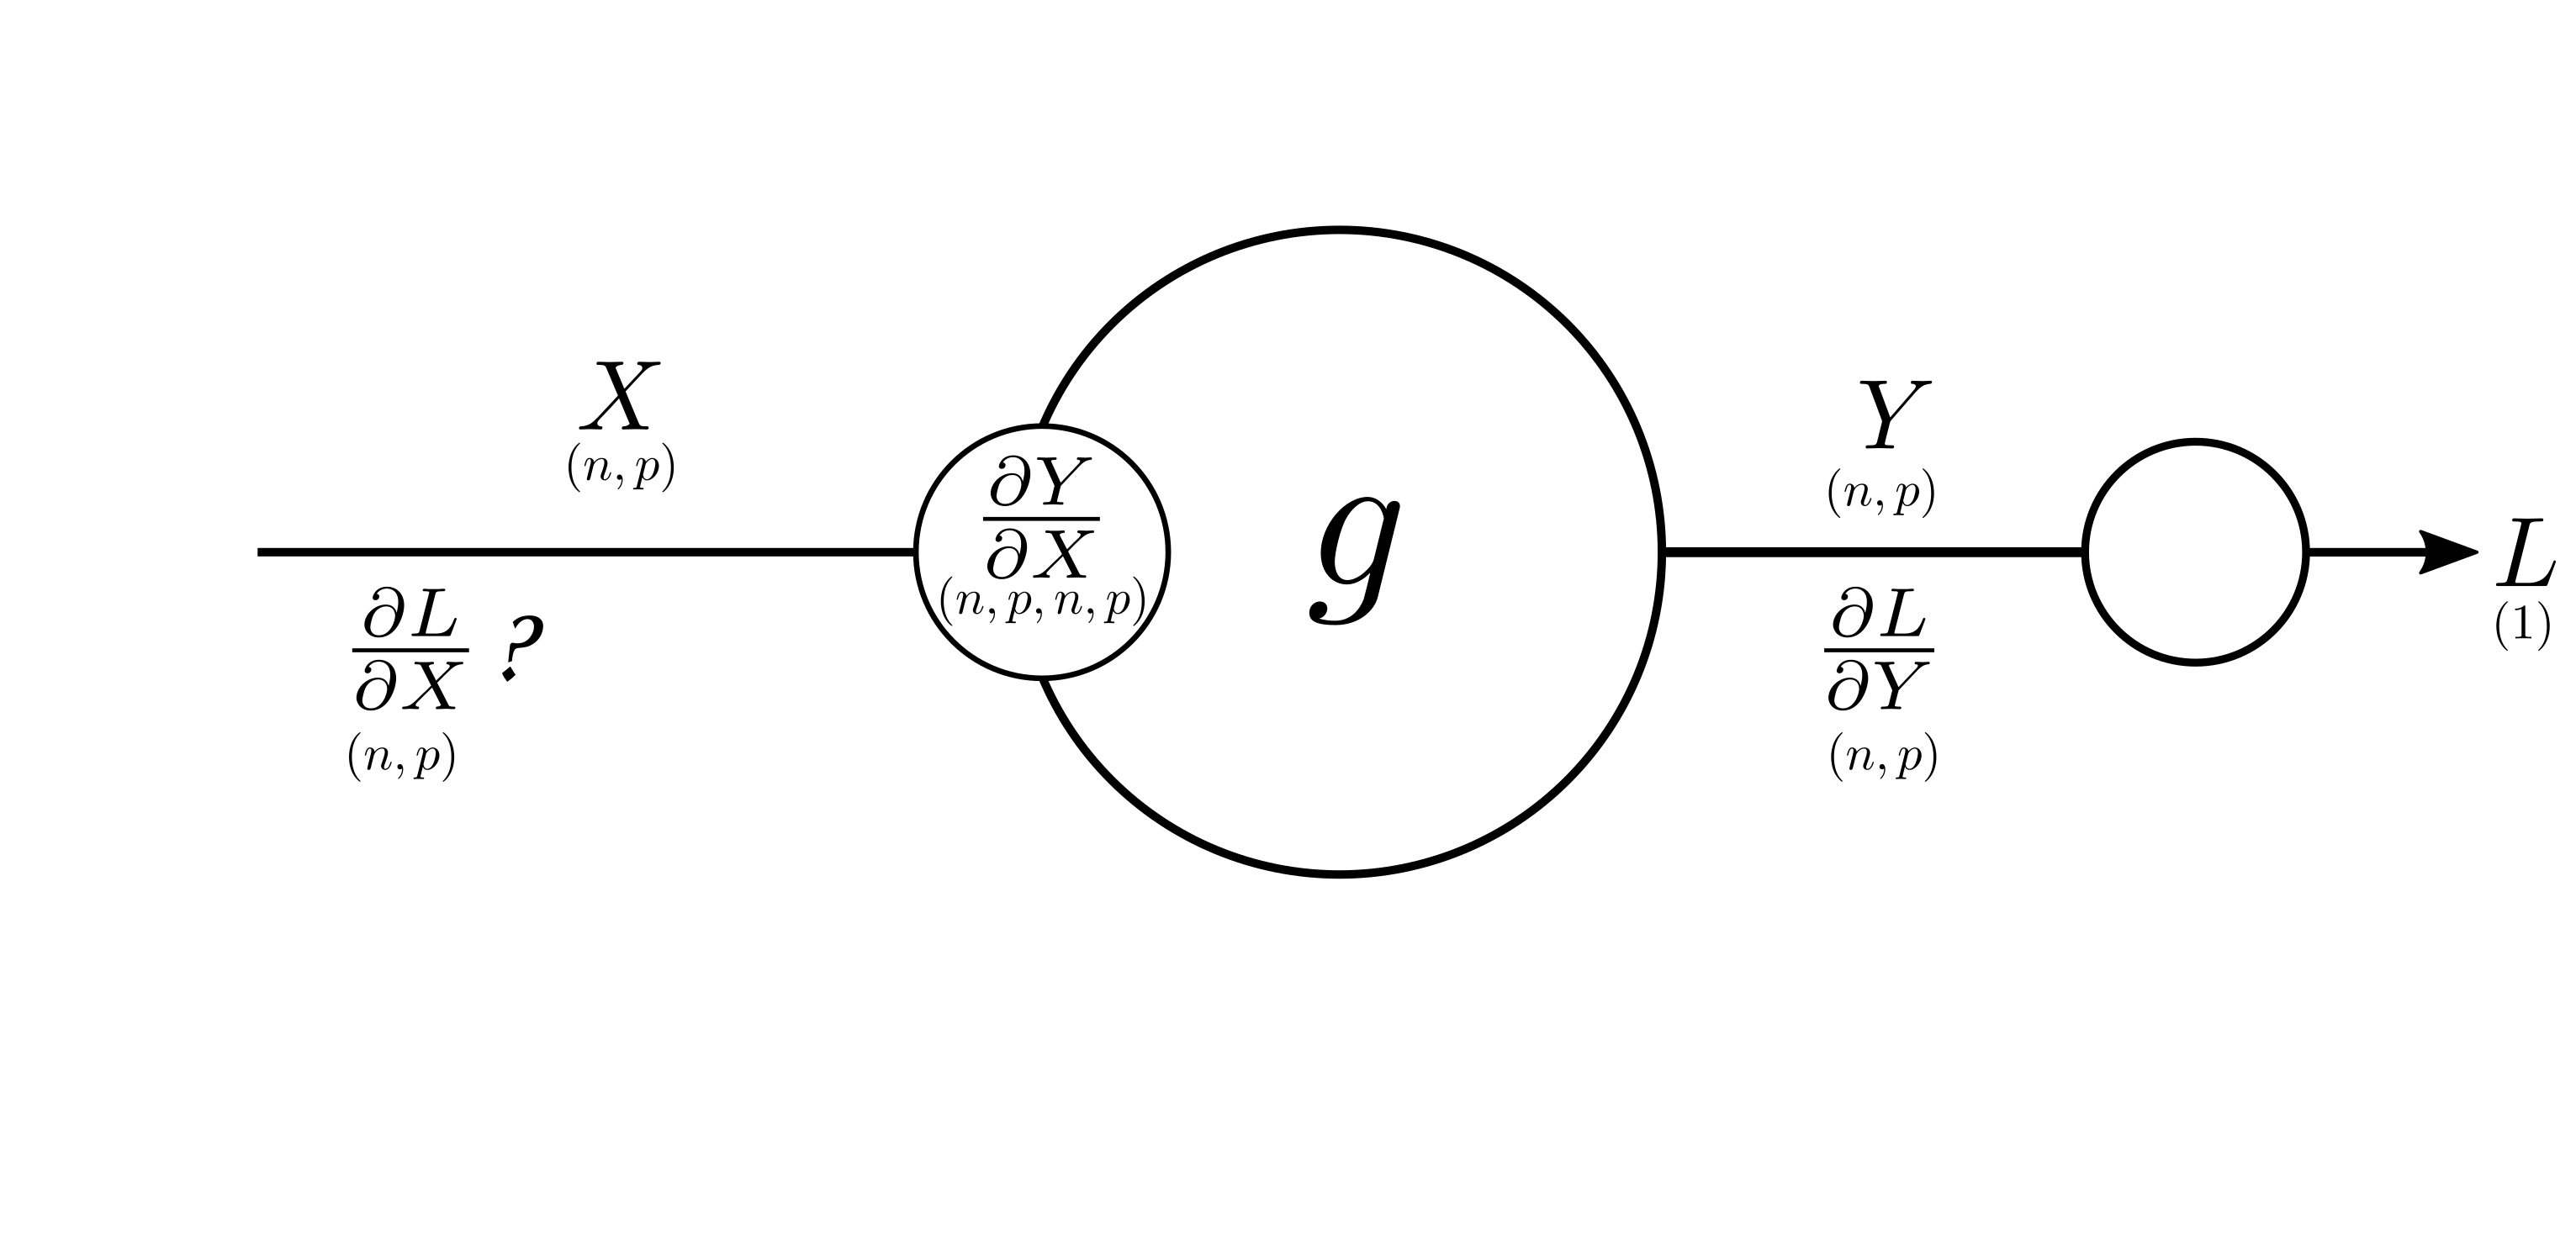
\includegraphics[width=0.8\textwidth]{bp_activation.png}
\end{figure}

\begin{itemize}
\item Computing the full matrix $\pdv{\Y}{\X}$ is impractical.
\item But here $Y_{i,j}$ only depends on $X_{i,j}$: $Y_{i,j} = \act(X_{i,j})$.
\item Therefore: $\pdv{\Y_{i,j}}{\X_{i,j}} = \act'$.
\item Finally:
\[
\pdv{\loss}{\X} = \pdv{\loss}{\Y} \odot \act'(\X) \text{ ,}
\]
where $\odot$ is the term by term matrix multiplication or Hadamard matrix multiplication.
\end{itemize}

\subsection{Backpropagation Through an Activation Function $g$}

\begin{figure}[h]
    \centering
    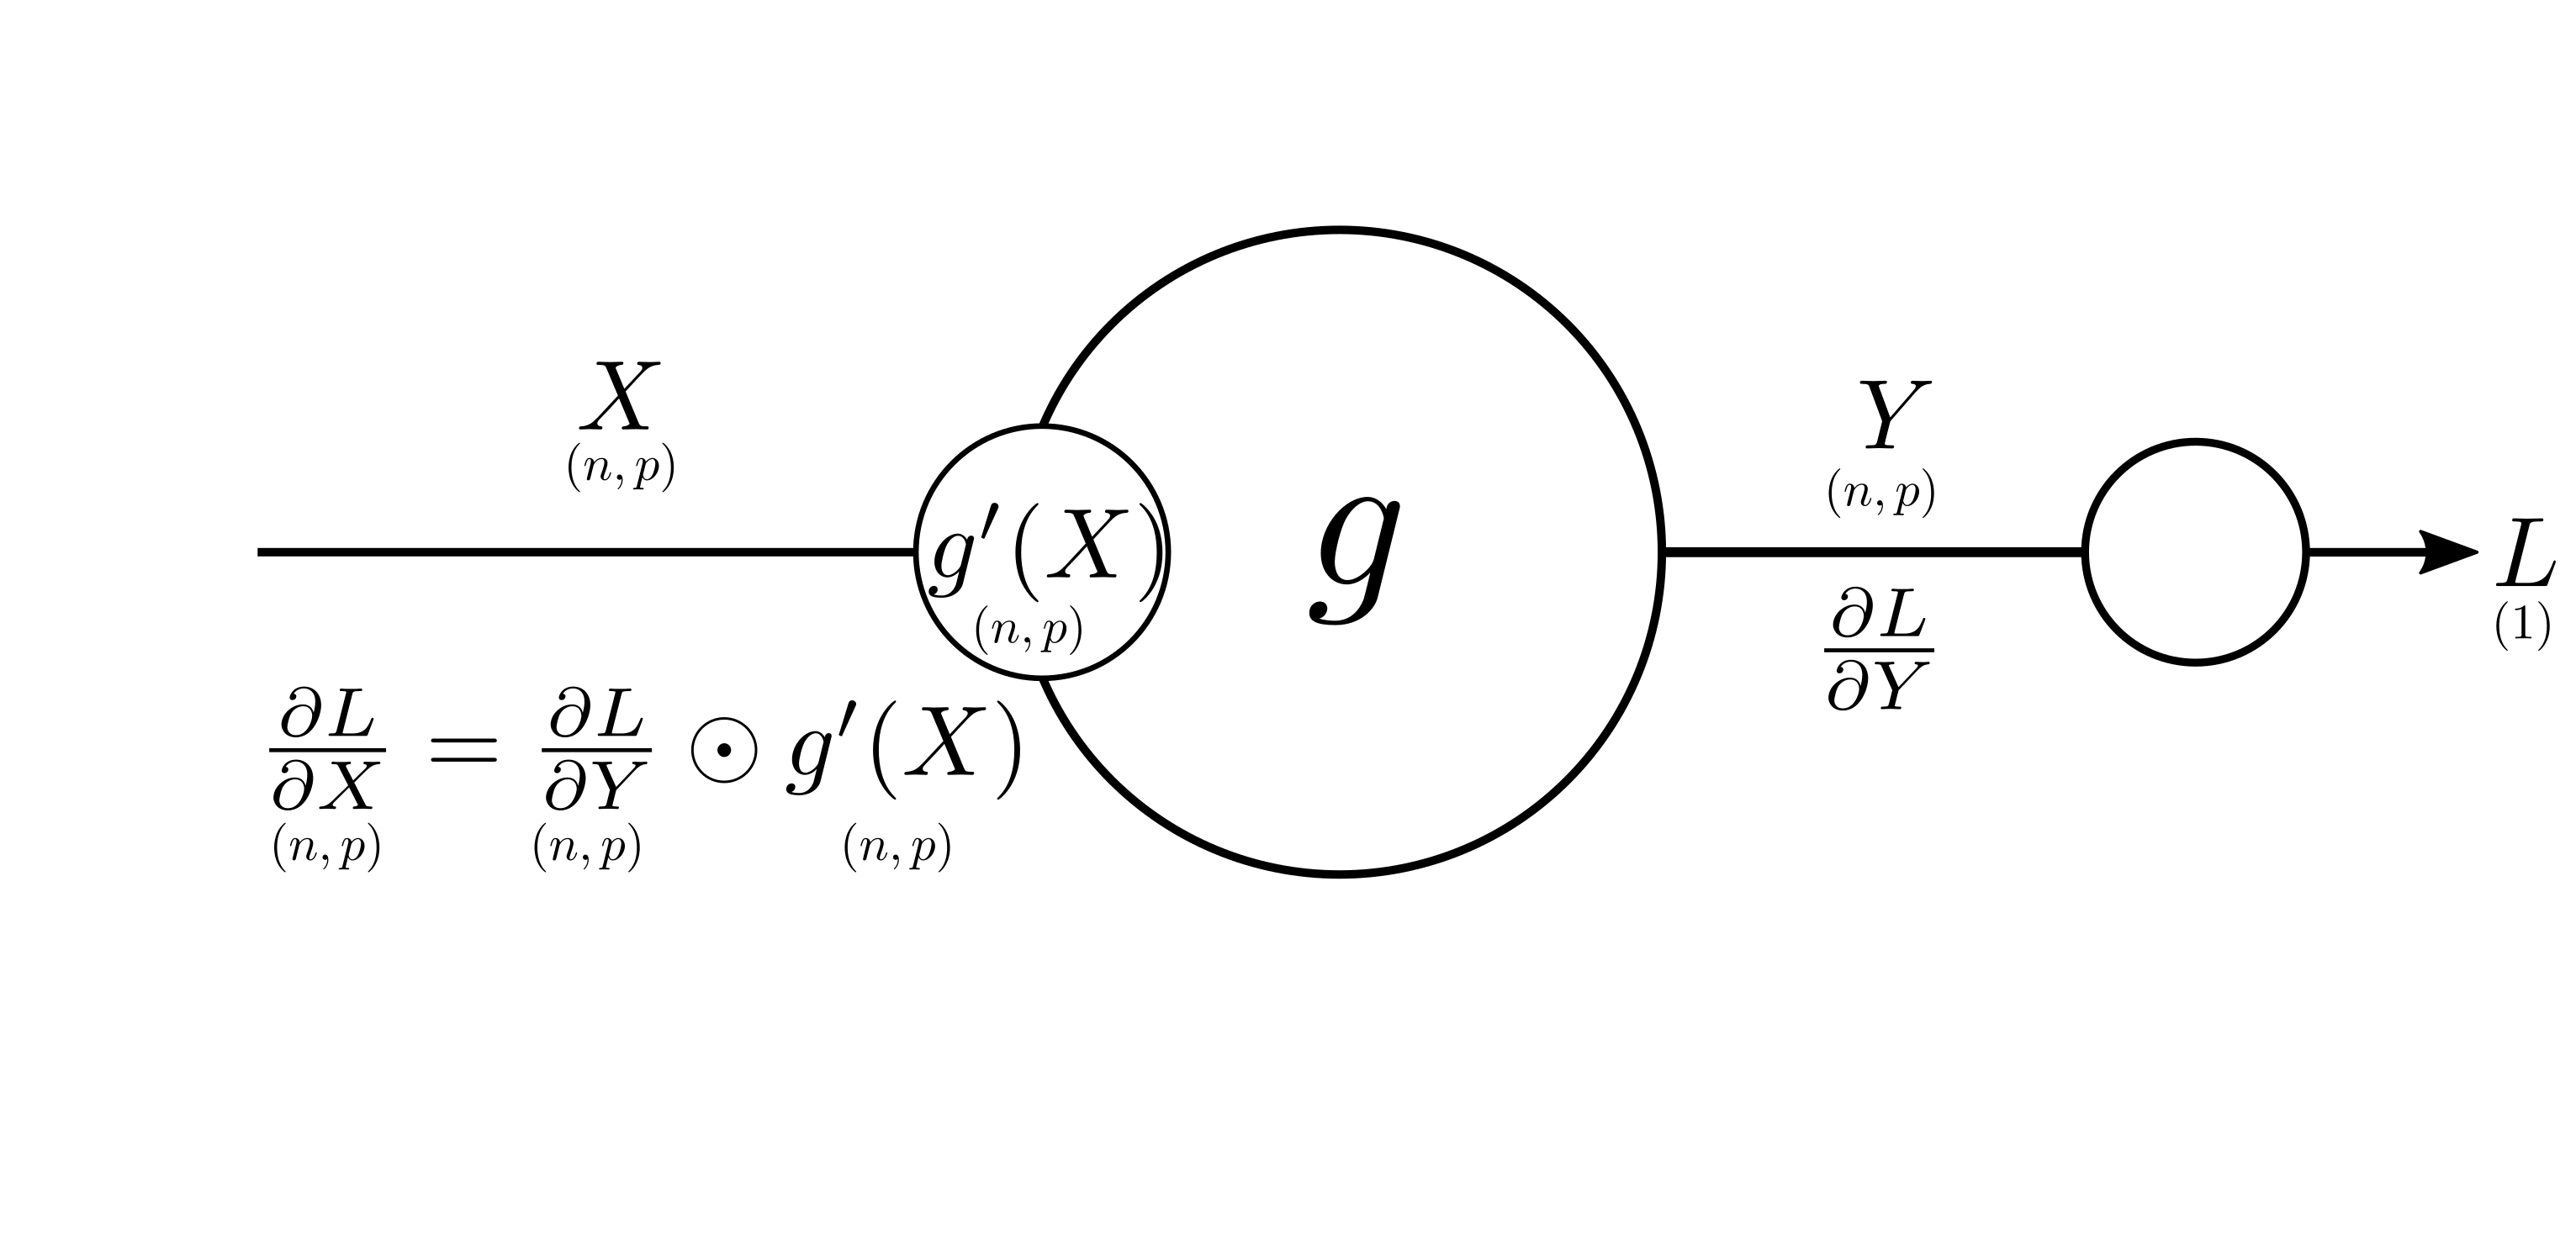
\includegraphics[width=0.8\textwidth]{bp_activation_2.png}
\end{figure}

\begin{block}{}
We will abusively write:
\[
\pdv{\Y}{\X} = \act'(\X)
\]
\end{block}

\subsection{Backpropagation Through a Matrix Product}

\begin{figure}[h]
    \centering
    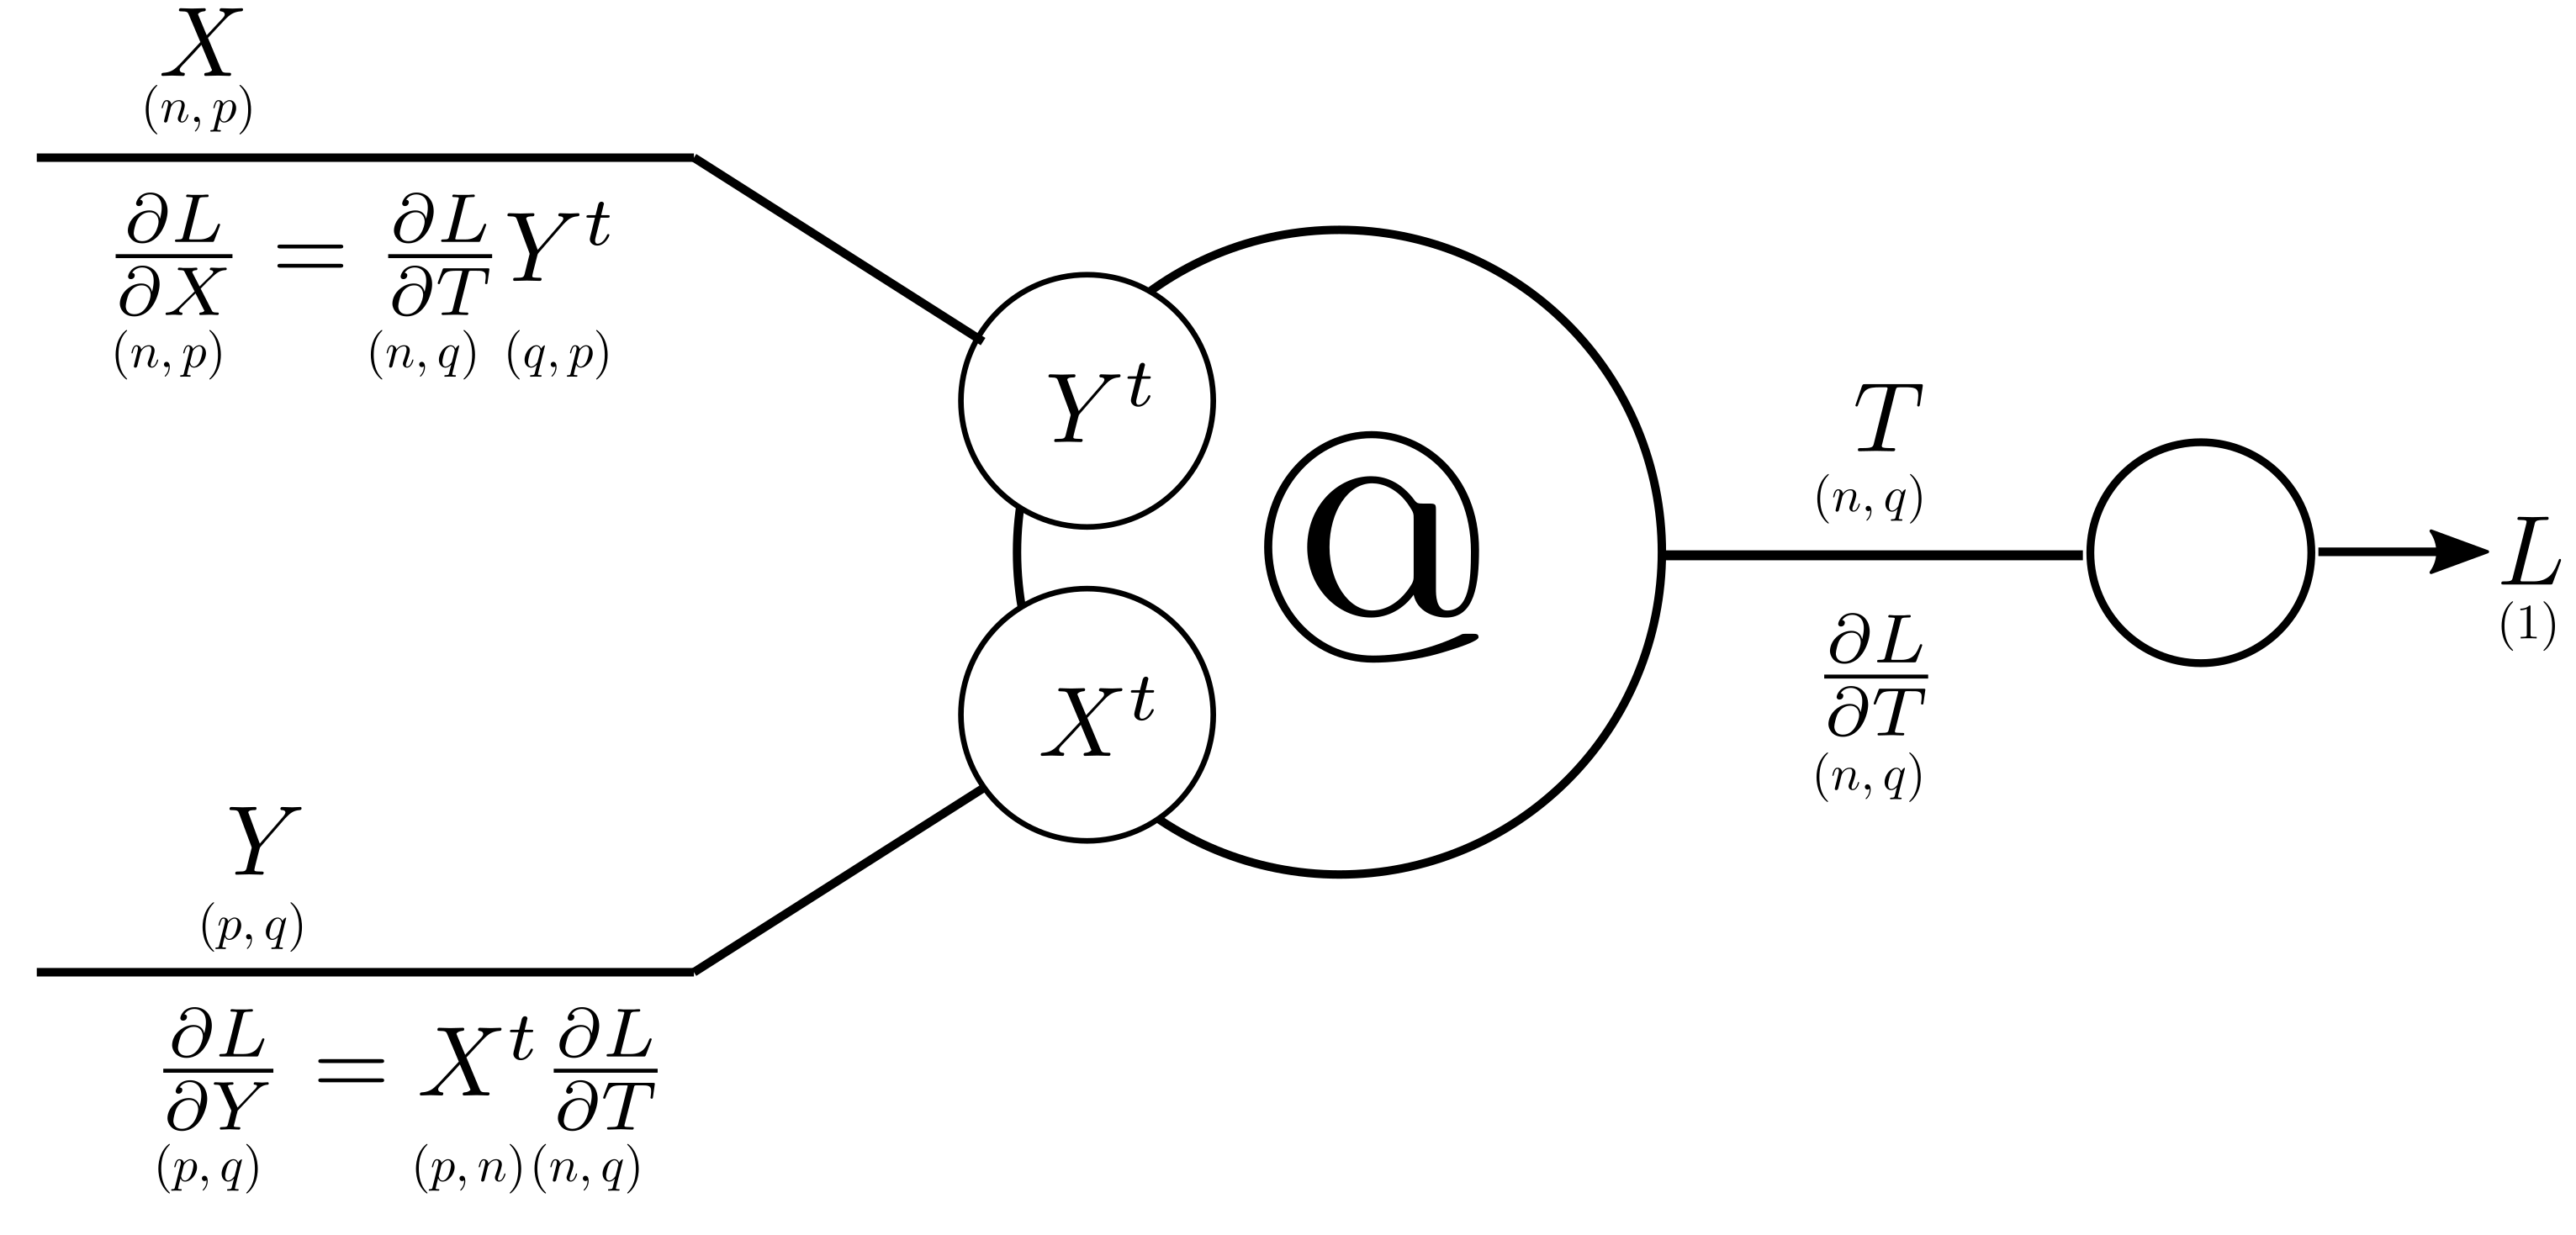
\includegraphics[width=0.8\textwidth]{matrix_mult_4.png}
\end{figure}

\begin{block}{}
We will abusively write, \alert{only for matrix multiplication}:
\begin{align*}
\pdv{\mathbf{T}}{\X} &= \Y^t \\
\pdv{\mathbf{T}}{\Y} &= \X^t
\end{align*}
\end{block}

\subsection{Backpropagation Through a Fully Connected Layer}

\begin{figure}[h]
    \centering
    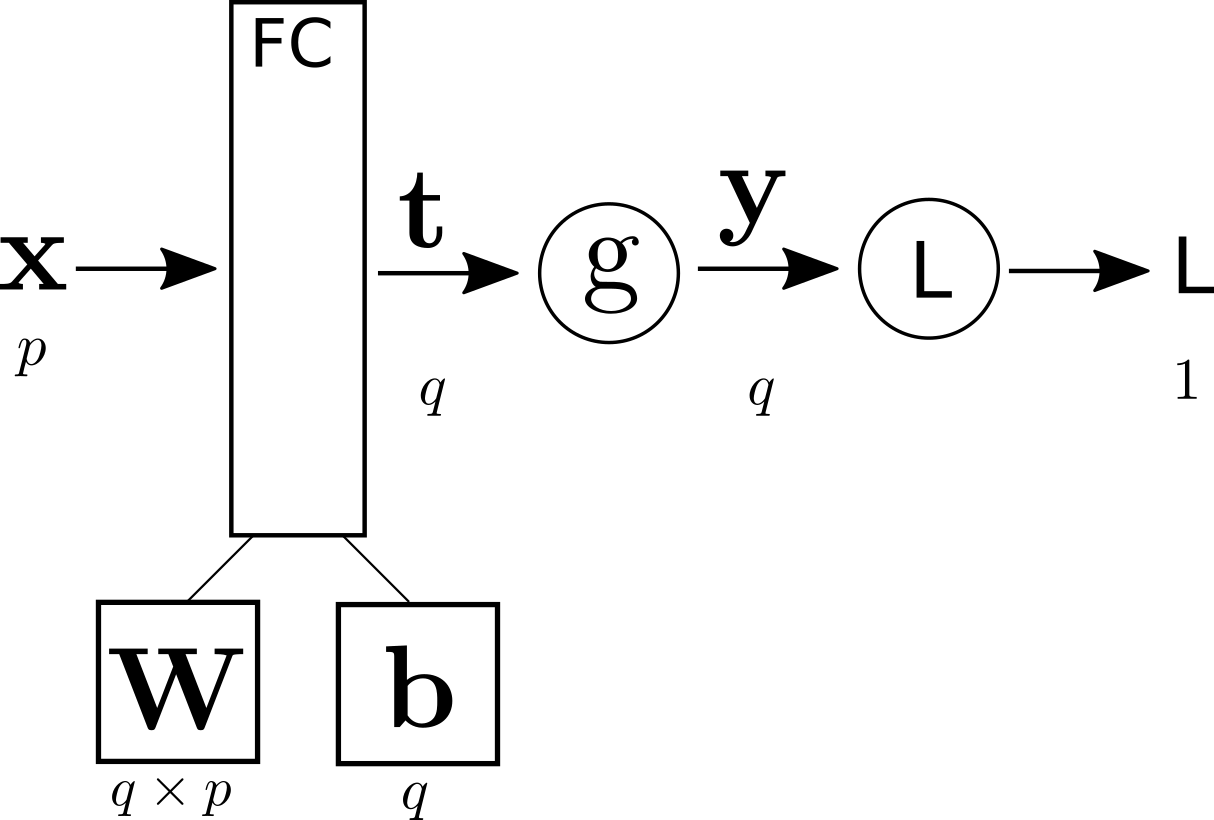
\includegraphics[width=0.5\textwidth]{bp_fc.png}
\end{figure}

\begin{columns}
\begin{column}{.5\textwidth}
Setup:
\end{column}
\begin{column}{.5\textwidth}
\begin{eqnarray*}
p, q \in \N^*\\
\x \in \R^p \\
\W \in \R^q \times \R^p \\
\bias, \mathbf{t}, \y \in \R^q \\
\loss \in \R
\end{eqnarray*}
\end{column}
\end{columns}

\begin{columns}
\begin{column}{0.5\textwidth}
Forward pass:
\begin{eqnarray*}
\mathbf{t} &=& \W\x + \bias \\
\y &=& \act(\W\x + \bias) \\
\loss &=& \loss(\y)
\end{eqnarray*}
\end{column}
\begin{column}{0.5\textwidth}
Local gradients:
\begin{eqnarray*}
\pdv{\mathbf{t}}{\W} &=& \x^t \\
\pdv{\mathbf{t}}{\bias} &=& Id_{(q)} \\
\pdv{\y}{\mathbf{t}} &=& \act'(\mathbf{t})
\end{eqnarray*}
\end{column}
\end{columns}

Backpropagation:
\begin{eqnarray*}
\pdv{\loss}{\mathbf{t}} &=& \pdv{\loss}{\y}.\pdv{\y}{\mathbf{t}} \\
&=& \pdv{\loss}{\y} \odot \act'(\mathbf{t}) \\
\end{eqnarray*}

Backpropagation:
\begin{columns}
\begin{column}{.5\textwidth}
\begin{eqnarray*}
\pdv{\loss}{\W} &=& \pdv{\loss}{\mathbf{t}}.\pdv{\mathbf{t}}{\W} \\
&=& \pdv{\loss}{\y} \odot \act'(\mathbf{t}).\x^t
\end{eqnarray*}
\end{column}
\begin{column}{.5\textwidth}
\begin{eqnarray*}
\pdv{\loss}{\bias} &=& Id^t . \pdv{\loss}{\mathbf{t}}\\
&=& \pdv{\loss}{\y} \odot \act'(\mathbf{t})
\end{eqnarray*}
\end{column}
\end{columns}

\section{Weights Initialization}

\subsection{Network Parameters Initialization}

\begin{block}{General Idea}
Inputs of activation functions should be in a range such that gradients are high.
\end{block}

\begin{columns}
\begin{column}{.3\textwidth}
\begin{figure}[h]
\centering
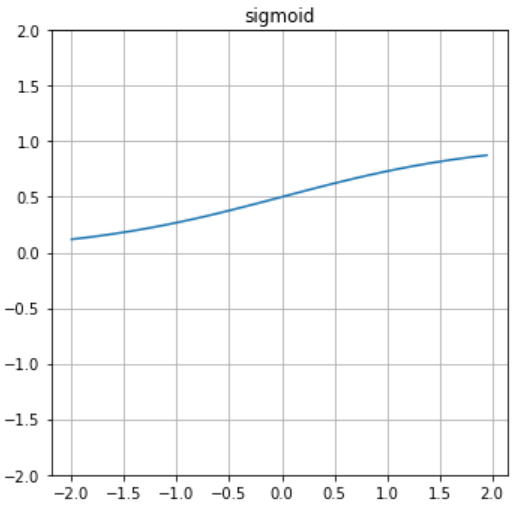
\includegraphics[width=\textwidth]{act_sigm.png}
\end{figure}
\end{column}
\begin{column}{.7\textwidth}
\begin{itemize}
\item Bias are set to zero.
\item If weights are also initialized to zero, then in each layer the activations will remain equal -- symmetry will never be broken.
\item Empirical solutions are based on a Gaussian distribution of the weights, with \textit{small} standard deviation.
\end{itemize}
\end{column}
\end{columns}

\subsection{Network Parameters Initialization: Current Practice}

\begin{itemize}
\item \cite{glorot_understanding_2010}: they empirically show that a standard deviation of $1/\sqrt{n}$ gives good results (where $n$ is the number of inputs of a neuron).
\item \cite{he_delving_2015}: in the case of ReLU activations, they recommend a $2/\sqrt{n}$ standard deviation.
\end{itemize}

\chapter{Conclusion}

We have seen:
\begin{itemize}
\item What is an artificial neuron and an artificial neural network (NN).
\item The (potential) power of a NN.
\item The backpropagation algorithm.
\item NN learning basics.
\end{itemize}

Next step:
\begin{itemize}
\item Application to images.
\end{itemize}

\bibliographystyle{apalike}
\bibliography{../../edf.bib}

\end{document}
